\documentclass [11pt, proquest] {uwthesis}[2016/11/22]
 
%
% The following line would print the thesis in a postscript font 

% \usepackage{natbib}
% \def\bibpreamble{\protect\addcontentsline{toc}{chapter}{Bibliography}}

\setcounter{tocdepth}{1}  % Print the chapter and sections to the toc
 

% ==========   Local defs and mods
%

\usepackage{alltt}  %

% packages added by xc
%\usepackage{subfiles}
\usepackage{amsmath} 
\usepackage{graphicx}
\usepackage{rotating}   % sidewaysfigure
\usepackage{multirow}  % for multirow cells in tables
\usepackage[flushleft]{threeparttable}   % for table notes
\usepackage{xr} % for cross reference
\usepackage{tabularx}

\newenvironment{demo}
  {\begin{alltt}\leftskip3em
     \def\\{\ttfamily\char`\\}%
     \def\{{\ttfamily\char`\{}%
     \def\}{\ttfamily\char`\}}}
  {\end{alltt}}
 
% metafont font.  If logo not available, use the second form
%
% \font\mffont=logosl10 scaled\magstep1
\let\mffont=\sf
% --- end-of-sample-stuff ---
 



\begin{document}
 
% ==========   Preliminary pages
\prelimpages
 
%
% ----- copyright and title pages
%
\Title{Understanding Probable Maximum Precipitation and Safety\\
  of Water Management Infrastructures under a Changing Climate}
\Author{Xiaodong Chen}
\Year{2017}
\Program{Department of Civil and Environmental Engineering}

\Chair{Faisal Hossain}{Professor}{Department of Civil and Environmental Engineering}
\Signature{Erkan Istanbulluoglu}
\Signature{L. Ruby Leung}

\copyrightpage

\titlepage

 
 % ----- abstract
%
\setcounter{page}{-1}
\abstract{%
Large water management infrastructures, such as high hazard dams located upstream of population centers, are usually designed according to the Probable Maximum Precipitation (PMP) criteria that are traditionally derived using historical records of extreme precipitation. Given the observed climate change in the past century and projected climate change in the next century, it is questionable whether the historical storms and the PMPs they derive are a reliable representation of present or future climate. On the other hand, the linear relationship between precipitation and precipitable water as assumed in the traditional method has been questioned in several studies. As a solution, atmospheric numerical modeling has been explored for physics-based PMP estimations, but no physics-based method has been well developed up to now, which makes the current studies appear ad-hoc. In this study, we establish a numerical modeling framework (based on Weather Research and Forecasting model) for extreme precipitation simulation, which lays the foundation of model-based PMP estimation. Using this modeling framework, we examine model reconstruction of various extreme precipitation events since 1905 and find that only those extreme storms after the 1940s can be satisfactorily reconstructed. This lays the basis for storm selection in the physics-based PMP estimation. Through statistical analysis of atmospheric reanalysis data, we examine the relationship between extreme precipitation and the atmospheric conditions, which provides region-specific guidelines to the physics-based PMP estimation. In this physics-based approach, either wind fields (in the western US) or moisture availability (in the eastern US) should be considered to reasonably maximize the storm magnitude. We also develop a hybrid method that bridges the traditional the physics-based methods, so a smooth transition is made possible for engineering communities. As a demonstration, we applied this hybrid approach to estimate the PMPs in the US Pacific Northwest region. The hybrid PMP estimates during 1970-2016 are similar to the traditional values, but the future PMPs will increase by $50\%\pm30\%$ of the current level by 2099 under the RCP8.5 scenario. Most of the increase is caused by warming, which mainly affects moisture availability through increased sea surface temperature. The findings of the study will help to modernize current engineering practice of PMP estimation and to better quantify the failure risk of large water management infrastructures for present and future climate scenarios.
}
 

% ----- contents & etc.
\tableofcontents
\listoffigures
\listoftables
 
% ----- glossary 
\chapter*{Glossary}       % starred form omits the `chapter x'

\addcontentsline{toc}{chapter}{Glossary}
\thispagestyle{plain}
%
\begin{glossary}

\item[ARW] Advanced Research WRF
\item[CAPE] Convective Available Potential Energy
\item[CMIP] Coupled Model Intercomparison Project
\item[CONUS] Contiguous US
\item[HMR] HydroMeteorological Report
\item[HU8] 8-digit Hydrolgic Unit
\item[PMP] Probable Maximum Precipitation
\item[PW] Precipitable Water
\item[RH] Relative Humidity
\item[WRF] Weather Research and Forecasting model

\end{glossary}
 
%
% ----- acknowledgments
\acknowledgments{% \vskip2pc
  % {\narrower\noindent
  I would like to thank my advisor Dr. Faisal Hossain for his encouragement and guidance during the past three years. I benefit so much from his passion and insight of research. I have enjoyed the years working with him, and I especially appreciate his patience to allow me to freely explore various interesting questions before sitting down with the current topic of this dissertation.
  
  I would like to thank my committee members Dr. Erkan Istanbulluoglu, Dr. Ruby Leung, and my two graduate school representatives, Dr. Joseph Cook, and Dr. Daehyun Kim for their invaluable feedback and suggestions along with my research. I want to also thank Dr. Cliff Mass, for bringing the new perspective to and sharing climate projections in my study.
  
  I want to also thank the members at the SASWE group. It has been a pleasure working with you, and you have been giving great suggestions on my research from time to time.
   
  %I am grateful to the friends I have met since I came to Seattle in 2011. Especially, I would like to thank Ted Bohn, Ben Livneh, Shrad Shukla, Mu Xiao
  
  Thank you to my family for their incredible support throughout my graduate studies, especially during my most difficult time. This dissertation cannot be completed without your support.
  
  At the time of writing, Chapter \ref{ch:JHE} has been published as \textit{Chen et al.} [2017] in the \textit{Journal of Hydrologic Engineering}, and Chapter \ref{ch:EF} has been published as \textit{Chen and Hossain} [2016] in the \textit{Earth's Future}. I would like to thank the \textit{Journal of Hydrologic Engineering}, published by the American Society of Civil Engineers, and the \textit{Earth's Future}, published by the American Geophysical Union, for granting the rights to include their articles as part of this dissertation.
  % \par}
}

%
% ----- dedication
%
\dedication{\begin{center}to my parents, Deying Li and Zhiyong Yang.\end{center}}

%
% end of the preliminary pages
 
 
 
% ==========      Text pages
\textpages
\chapter {Introduction}
\label{ch:intro}

\section {Background information}

Extreme precipitation, or heavy rainstorms as sometimes referred, are those that happen very rarely. They account for a considerable part of annual precipitation at a given location. From the perspective of magnitude, heavy storms are defined using the hourly rainrate of 7.6mm/hr [\textit{Huschke}, 1959].

Over the past century, numerous water infrastructures have been built to serve the water-related need of people worldwide [\textit{Mitchell}, 1990]. Those larger ones often serve multiple purposes, such as agriculture, navigation, hydropower, and flooding control. Failure of such high-hazard dams would bring catastrophic eco-societal loss. Therefore, they are often the center of local and regional water resources management [\textit{Asmal and Coauthors}, 2000; \textit{Grigg}, 1996]. For example, the failure of the South Fork dam in Pennsylvania, USA in 1889 caused 2,209 deaths and an economic loss of 17 million dollars [\textit{Frank}, 1988; \textit{VandenBerge et al.}, 2011].  For these infrastructures, Probable Maximum Precipitation (PMP), or Probable Maximum Flood (PMF) which can be derived from PMP,  has been widely used to ensure its safety under the extreme weather conditions [\textit{Hossain et al.}, 2012]. PMP is also a widely used design criteria for the nuclear water disposal sites, as any leakage from the failure of site/equipment is not tolerable [\textit{Hayes et al.}, 2015].

Probable Maximum Precipitation (PMP) follows an idea of creating an extreme scenario that covers all the possibilities. In the engineering practice, the definition by the World Meteorological Organization (WMO) is often adopted: probable maximum precipitation is the ``theoretical maximum precipitation that a given watershed can receive in a given duration of time''. Besides this definition, WMO also gives detailed instructions on how to make PMP estimation using various approaches [\textit{World Meteorological Organization (WMO)}, 1986]. In general, they can be classified into: local method (maximization of local storms), transposition method (storm transposition from same climatological regions), generalized method (based on some provided PMP distribution maps), as well as statistical method such as the one proposed in \textit{Hershfield} [1965]. At the national scale, different countries adopt different methods for their own PMP estimation. For example, PMP in India follows the generalized PMP approach [\textit{Rakhecha and Kennedy}, 1995; \textit{Rakhecha and Singh}, 2009], with the adjustment carried for the impact of local topography. In the US, moisture maximization method is chosen by NOAA as the standard approach, and NOAA has published a series of instructions for different climatological regions, now known as HydroMeteorological Reports (HMRs).

The moisture maximization approach estimates PMP as equation \ref{eq:1-1}, where $P$ is the observed precipitation, $PW$ is the observed maximum 12-hour persisting precipitable water in the storm duration, and $PWm$ is the climatological 12-hour persisting precipitable water at this location. In practice, $PW$ and $PWm$ are estimated from surface dew point temperature measurement, assuming a pseudoadiabatic air condition. From long-term ground observations, the most severe rainstorms in the history are maximized following this equation, and the maximum of these derived values are defined as the PMP of this site. At certain HMR regions where surface topography plays important roles in the storming process (such as the watersheds along the west coast), the topographic adjustment is applied as appropriate.

\begin{equation}
PMP = P \times{\frac{PWm}{PW}}
\label{eq:1-1}
\end{equation}

In the recent decades, this moisture maximization approach has been revisited with high-quality observation and advanced atmospheric modeling. For example, \textit{Abbs} [1999] used atmospheric model and checked the linear assumption assumed in equation \ref{eq:1-1}. This study found that such linear assumption may introduce bias in the maximization procedure. On the other hand, the storm efficiency during the observed extreme precipitation events are often between 80\% and 100\%. Thus the moisture maximization does not fully release the precipitation potential. \textit{Chen and Bradley} [2006] analyzed observation data and concluded that surface dew point temperature plus pseudoadiabatic assumption tend to overestimate $PW$ of the air column.

As a response to these concerns, numerical modeling has been proposed as an alternative to the traditional approach. As a basis of model-based PMP estimation, model reconstruction of extreme precipitation has demonstrated its capability across various extreme rainfall events across the world in the past several decades [\textit{Kato}, 1998; \textit{Rao et al.}, 2007; \textit{Vaidya and Kulkarni}, 2007; \textit{Kumar et al.}, 2008; \textit{Chang et al.}, 2009; \textit{Pennelly et al.}, 2014; \textit{Li et al.}, 2017; \textit{Yang et al.}, 2017]. With good quality input data (i.e., initial and boundary conditions to the simulation), modern atmospheric models can reconstruct the spatial-temporal rainfall pictures in the context of various weather systems (e.g., atmospheric rivers, cyclones/tornadoes, mesoscale convective systems, topographic precipitation). Along with high-quality rainfall pictures, models also provide complete information on the related meteorological diagnostic variables (such as air temperature, wind fields, and precipitable water as used in equation \ref{eq:1-1}). Numerical models do not require ground observation data as direct input (though ground observation is highly useful in the data assimilation procedures that generate the input to these numerical models). Therefore it is capable of reconstructing the extreme events since the 1940s given the current availability of model input datasets. Several other datasets, such as the 20th century reanalysis products (20CRs), even enable us to look into the weather events of as early as the 1850s. They potentially provide more complete datasets of extreme events and more quality-consistent data of precipitation/diagnostic variables as compared with ground observations on the scale of centuries. There have been studies checking the data quality of the 20CRs, as well as modeling efforts on the storms as old as in the 1960s [\textit{Yang et al.}, 2017]. However, up to now, no studies have been done to quantify the usability of these datasets in the extreme event simulations for the early periods (before the 1940s or even the 1900s).

As the science/engineering communities get concerned with the ongoing climate change in the recent decades, atmospheric models with climate projections can also reveal the future of the extreme events under climate change. For example, \textit{Warner et al.}, 2015 looked into the extreme precipitation in the US Pacific Northwest region duirng 1970-2000 and 2070-2100 using CMIP5 models, and found that precipitable water (the moisture source of precipitation) is going to increase by 15\% to 39\% in the future. Kunkel et al. [2013] used CMIP5 results to investigate the PMP in the future, and found that both moisture avaibility and atmospheric vertical winds would increase in the future, suggesting a potential increase of PMPs. Study by \textit{Rastogi et al.} [2017] took this approach further and investigated the possible change of PMP design standard in the Alabama-Coosa-Tallapoosa river basin in the southeast US.

Based on good constructions of extreme precipitation events, a number of ways to modify the model and make model-based PMP estimations have been proposed. In general, these approaches can be classified into 3 categories: 1) disturbance of air moisture through changing air temperature/relative humidity and keeping the atmospheric columns throughout the simulation domain fully moist during the storm events [\textit{Ohara et al.}, 2011; \textit{Tan}, 2010]; 2) disturbance of moisture flux through changing wind speed or wind fields [\textit{Ishida et al.}, 2015]; 3) combination of worst historical environmental conditions [\textit{Tan}, 2010]. However, all these studies are based on the ``trail and error'', and the largest maximized precipitation amount is taken then as PMP value. Since there has been no comprehensive study to date that investigates the key atmospheric conditions that affect extreme storms (e.g., moisture availability, atmospheric instability, large-scale convergence), the engineering community is still left without a rational guideline on the use of numerical models for PMP estimation. In other words, studies that can derive systematic and detailed guidance as those in HMRs are required.

In summary, for the engineers to complete the switch to the model-based PMP estimation approach, the following challenges need to be addressed:

1. Unlike land surface hydrological modeling, atmospheric models usually involve parameterization schemes to approximate the atmospheric processes (e.g., water phase transition, sub-grid scale convections). Therefore, what would be a good modeling framework that can be easily adopted by engineering for rainfall simulations? What storms can we now confidently construct given the current reanalysis/projection data?

2. Physics-based methods should be developed to estimate PMP in the numerical models. The current trail-based approach needs to be replaced with more physics-based and more convincing approaches that are based on the understanding of storm processes and local climatology.

3. A smooth transition from the traditional approach to the proposed model-based approach is required. There have been thousands of large water infrastructures designed using traditional PMP criteria. Therefore, it is critical that we understand what has changed, while what is kept in the new model-based approaches (figure \ref{fig:1-1}). Only by this way can we connect the model-based PMPs to the safety of existing infrastructures in the future.


\begin{figure}[htbp]
	\centering
	\includegraphics[width=\linewidth]{pics/ch1/fig1.png}
	\caption{A complete transition from traditional approach to physics-based approach of PMP estimation.}
    \label{fig:1-1}
\end{figure}

\section {Objectives}

Through this dissertation, I hope to have a better understanding of the relationship between extreme precipitation and the environmental conditions. Taking this information into atmospheric numerical modeling, I hope to help the engineering community to get ready to utilize numerical model for infrastructure safety evaluation. To be specific, I hope to achieve the following goals:

1. To establish a numerical modeling framework for extreme rainfall event simulation in engineering practice.

2. To develop a method to physically estimate PMP while accounting for uncertainties for engineering practice.

3. To estimate PMP change as a function of the climate change.



\section {Approach}

The core of this dissertation is organized as follows:

Chapter \ref{ch:JHE} presents a numerical modeling framework (based on WRF) for engineering extreme precipitation events investigation. Chapter \ref{ch:EF} takes this framework and examines out capability of reconstructing the extreme precipitation events in the history. These two chapters lay the foundation of model-based storm construction and thus PMP estimation. Chapter \ref{ch:JHM} performs a statistical analysis of the historical extreme precipitation as reflected by the major reanalysis products, and reveals the spatially heterogeneous relationship between extreme precipitation and the environmental conditions. Chapter \ref{ch:WRR} develops the hybrid approach in figure \ref{fig:1-1}, and links the current and proposed PMP estimation approaches. Chapter \ref{ch:con} presents the findings from the collection of research and the recommendations to future studies.
\chapter {Preparation of Numerical Modeling Framework for Engineering Extreme Storm Analyses}
\label{ch:JHE}
 
This chapter has been published mostly in its current form in the \textit{Journal of Hydrologic Engineering}. \textcopyright American Society of Civil Engineers. Used with permission.\\

\bigbreak

\noindent
\hangafter=1
\setlength{\hangindent}{2em}
Chen, X., Hossain, F., and Leung, R. L. (2017), Establishing a Numerical Modeling Framework for Hydrologic Engineering Analyses of Extreme Storm Events, \textit{Journal of Hydrologic Engineering}, 22(8), 04017016. doi:10.1061/(ASCE)HE.1943-5584.0001523.

\vspace{10mm}

\noindent
\textit{\textbf{Abstract}}
 
In this study a numerical modeling framework for simulating extreme storm events was established using the Weather Research and Forecasting (WRF) model. \
Such a framework is necessary for the derivation of engineering parameters such as probable maximum precipitation that are the cornerstone of large water management infrastructure design. \
Here this framework was built based on a heavy storm that occurred in Nashville (USA) in 2010, and verified using two other extreme storms. \
To achieve the optimal setup, several combinations of model resolutions, initial/boundary conditions (IC/BC), cloud microphysics and cumulus parameterization schemes were evaluated using multiple metrics of precipitation characteristics. \
The evaluation suggests that WRF is most sensitive to IC/BC option. Simulation generally benefits from finer resolutions up to 5 km. \
At the 15-km level, NCEP2 IC/BC produces better results, while NAM IC/BC performs best at the 5-km level. \
Recommended model configuration from this study is: NAM or NCEP2 IC/BC (depending on data availability), 15km or 15km-5km nested grids, Morrison microphysics and Kain-Fritsch cumulus schemes. \
Validation of the optimal framework suggests that these options are good starting choices for modeling extreme events similar to the test cases. \
This optimal framework is proposed in response to emerging engineering demands of extreme storm events forecasting and analyses for design, operations and risk assessment of large water infrastructures.

\vspace{20mm}

\section{Introduction}
 
Intense storms, or extreme rainfall events as we shall call them hereafter, pose challenges to infrastructure management and design, and trigger other catastrophic events such as floods, landslides and dam failures [\textit{Evans et al.}, 2000; \textit{Casagli et al.}, 2006; \textit{Cong et al.}, 2006]. They are also the cornerstone of engineering design and risk assessment of large infrastructures such as dams, levees, and power plants [\textit{Stratz and Hossain}, 2014]. Therefore, it is of great societal interest to physically predict and understand the occurrence and magnitude of such extreme events for both design and operation of engineering infrastructures.

In current engineering practice, the safety of hazardous infrastructure (where lives are at stake with infrastructure failure) is achieved through designs based on Probable Maximum Precipitation ($PMP$). $PMP$ is defined as the theoretical greatest depth of precipitation for a given duration that is physically possible over a particular drainage area [\textit{Huschke}, 1959]. It depicts the precipitation potential of an already intense storm that is ‘maximized’ to an upper bound using some basic engineering assumptions [\textit{Kunkel et al.}, 2013; \textit{Stratz and Hossain}, 2014]. The National Oceanic and Atmospheric Administration (NOAA) has created a database of such intense storms in the United States from about 1900-1990 that were maximized to $PMP$s and publicly released as Hydrometeorological Reports (HMRs) for the engineering infrastructure community [\textit{U.S. Department of Commerce}, 1999]. For engineering practices outside the US, the World Meteorological Organization have outlined several approaches that can be used [\textit{World Meteorological Organization (WMO)}, 1986]. In general, these are local method (maximization of local storms), transposition method (storm transposition from same climatological regions), generalized method (based on some provided $PMP$ distribution maps), as well as statistical method such as the one proposed in Hershfield [1965].

$PMP$ is generally expressed mathematically as: $P×W_p(maximum)/W_p(storm)$, where P is the observed rainfall accumulation, wp(maximum) is the highest observed precipitable water from historical records and wp(storm) is the storm precipitable water. The above approach is often criticized as being insufficiently physical as it assumes a linear relationship between precipitation and water holding capacity of the atmosphere [\textit{Abbs}, 1999; \textit{Kunkel et al}., 2013]. Also it heavily relies on historical observation data. For very early extreme events used in PMP analysis (such as Storm Elba of 1929), it is difficult to obtain a physically consistent picture due to limitations of record keeping and the linearity assumption [\textit{Abbs}, 1999]. In this context, numerical simulation of extreme storms and their consequent physical maximization to a ``$PMP$" is gaining much more traction among science and engineering communities than before [\textit{Kunkel et al.}, 2013; \textit{Stratz and Hossain}, 2014].

Numerical modeling approach has several key advantages over the traditional approaches. It is able to produce finer details on the spatial-temporal structure of the storms using fewer assumptions and experience-based estimation. It is more tailored to a region that has little or no long-term rainfall record or is rapidly undergoing changes in weather patterns due to land cover change or global warming. More importantly, a well-established numerical modeling framework is often able to handle various extreme events within the model domain spanning decades [\textit{Chen and Hossain}, 2016]. In the study of \textit{Tan} [2010], the WRF model was calibrated and setup over American River basin. It was found capable of simulating various PMP-class storms in the basin during 1970-2000. The model also provided better space-time pictures of the historical events that were used in HMRs for PMP estimation in this basin. This is another benefit from numerical modeling approach.

There have been numerous studies on extreme events/PMPs using numerical atmospheric models. Some conclusions have been reached on the optimal setup of numerical models. For example, optimal grid size ratios of 1:7, 1:5 and 1:3 were validated over 8 storms in southwest England [\textit{Liu et al.}, 2012]. The study by \textit{Pennelly et al.} [2014] concluded that for storms in Alberta, Canada, 6km grids in the WRF model is a balance between simulation quality and time expense. There have also been efforts in optimizing the simulated rainfall results by operating model with more information. For example, \textit{Giannaros et al.} [2016] assimilated lightning data into the atmospheric numerical simulation, and it helped improve precipitation forecast. However, a consistent framework informing the users from the hydrologic engineering community ``how to systematically set up and analyze numerical models" for engineering analyses is still absent in the literature.

Previous studies suggest that the performance of storm simulation heavily depends on the parameterization schemes, which is the mathematical identification of physical processes in the numerical models [\textit{Stensrud}, 2009]. Though a wise choice of parameterization schemes results in improved simulations of big storms, often it has to be achieved by trial and error. For example, several numerical studies for the Mumbai July 2005 storm [\textit{Rao et al.}, 2007; \textit{Vaidya and Kulkarni}, 2007; \textit{Kumar et al.}, 2008; \textit{Chang et al.}, 2009] show steady progress in reconstructing the high precipitation values in the various modeling platforms with different parameterization schemes. \textit{Rajeevan et al.} [2010] revealed that the optimal combinations of parameterization schemes and IC/BC in the model can be quite different for the southeast Indian thunderstorms. These high heterogeneities within optimal model configurations make it difficult for engineering communities to setup and operate these models.

Given that the engineering community is relatively new to the setup/operation of numerical models, as well as the use of models for maximization of extreme storms in PMP estimation, a framework to explore the role of various parametrizations and IC/BC on extreme storm simulation accuracy can provide a baseline for optimal criteria for PMP simulation. Such a comprehensive study will also illustrate ways to identify optimal model configurations for extreme storm simulations, and help the engineering infrastructure community that engages in hydrologic analyses for design and operations embrace numerical models for $PMP$ estimation and further advance the methodology.

In this chapter, we investigate ways to establish a generic numerical modeling framework over a given area. Taking the Nashville, USA 2010 storm as a test case, we illustrate procedures required to achieve a good storm reconstruction using WRF model. We evaluate various combinations of parameterization schemes, IC/BCs and grid sizes. Using this framework, we address three questions:

1. What combinations of model options in WRF are most skillful for extreme storm event simulation?

2. What are the strengths and weaknesses of each model option in reference to simulation accuracy of extreme precipitation? 

3. What are the optimal model configurations for engineering operations and infrastructure implications?
 
 
\section{Nashville, USA 2010 extreme storm}
 
During May 1 and May 2, 2010, the west and middle Tennessee region of the USA experienced a record-breaking storm. This 2-day rainfall event brought huge amount of water to western Tennessee, with 48-hour cumulative rainfall exceeding historical records at several gauge stations (such as the Nashville and Camden station at Tennessee). Figure \ref{fig:2-1} shows the 48-hour cumulative rainfall from this storm as observed from NEXRAD network, which shows a southwest-northeast pattern.

This storm, hereafter referred to as ``Nashville 2010 storm", lead to a flood in the following days that NOAA categorized as a 1000-year return period flood event [\textit{NOAA National Weather Service and Weather Forecast Office, NWSWF}, 2010]. The maximum 48-hour total precipitation observed was 493 mm (19.41 inches) at the Camden COOP station ($36.05^{\circ}$N, $88.08^{\circ}$W, the red star in Figure \ref{fig:2-1}). This value is quite close to the 5,000 mi2 48-hour design $PMP$ (495 mm, or 19.5 inches) for west Tennessee (an area in HMR 1951 report; we will call it as HMR51 region hereafter). Nashville international airport recorded its 1st and 3rd highest 24-hour total rainfall in the history on 1 and 2 May [\textit{NWSWF}, 2010]. These statistics qualify this rainfall event as a reference extreme storm for $PMP$ design for the HMR51 region. During the ensuing flood event, 21 deaths were reported, and over 30 counties were declared as major disaster areas by the government. This unique rainfall record and infrastructure-damaging impact make this event worth revisiting with numerical simulation [\textit{Durkee et al.}, 2012]. There have not been many numerical simulation efforts on this storm. Thus a successful model reconstruction of this event would provide an important baseline for studying other local events or events in similar environmental conditions for engineering infrastructure applications.

\begin{figure}[htbp]
	\centering
  	\includegraphics[width=13cm]{pics/ch2/fig1.jpg}
  	\caption{48-hour (0000 UTC 1 May–0000 UTC 3 May, 2010) total rainfall from Stage IV data (unit: mm).}
  	\label{fig:2-1}
\end{figure}

The Nashville 2010 storm was among a series of big storms (tornado 41, 43 and 57) hitting the mid-southern US in the same period. Analysis of reanalysis products suggests that the event was associated with a synoptic system with significant atmospheric moisture. The Atlantic ridging associated with the negative-phase of the North Atlantic Oscillation (NAO) helped amplify and slow the eastward propagating synoptic wave pattern that generated heavy precipitation from mesoscale organized convective systems [\textit{Durkee et al.}, 2012]. An atmospheric river originating from the Intertropical Convergence Zone (ITCZ) in Central America provided the moisture source for this record-breaking event [\textit{Durkee et al.}, 2012]. Surface topography in the Appalachians provided orographic forcing for moisture convergence and land surface heating helped maintain atmospheric instability so precipitation continued until 2 May, 2010. Previous studies have identified several key atmospheric factors such as the superposition of the polar/subtropical jet [\textit{Winters and Martin}, 2014] and the atmospheric river [\textit{Durkee et al.}, 2012; \textit{Moore et al.}, 2012]. Because some elements present in the Nashville 2010 event are common ingredients in other extreme storms, reconstructing this extreme event may serve as an important test case for evaluating the ability of the WRF model for simulating other storms.

\section{The numerical atmospheric model}

WRF model is employed for the big storm reconstruction. WRF is an atmospheric modeling system [\textit{Skamarock et al.}, 2008] that features two non-hydrostatic solvers including the Advanced Research WRF (ARW) core for atmospheric research, and the Non-hydrostatic Mesoscale Model (NMM) core for the operational forecast. In this study we adopted WRF-ARW v3.6.1 for the storm simulation. WRF-ARW has been employed in various big storms studies and demonstrated to be capable of simulating several big storms across the world [\textit{Kumar et al.}, 2008; \textit{Rajeevan et al.}, 2010; \textit{Tan}, 2010; \textit{Chen and Hossain}, 2016].

WRF-ARW is designed for mesoscale meteorological simulation with spatial resolution ranging from 1km to 100km. Accordingly, the time step used in the model varies from seconds to minutes. It simulates the atmospheric motion using compressible, non-hydrostatic Euler equations with consideration of mass, energy and momentum conservation. These equations are formulated and solved using the Arakawa-C grid with terrain-following mass vertical coordinate [\textit{Laprise}, 1992]. WRF-ARW uses various parameterization schemes to estimate the atmospheric processes at sub-grid scale, and atmospheric moisture is considered in various phases in the cloud microphysics parameterization schemes. For example, in the Morrison microphysics scheme, water is considered in vapor, cloud droplets, cloud ice, rain, snow, and graupel/hail phases [\textit{Morrison et al.}, 2009]. This ensures an accurate description of moisture in the air. By default, WRF-ARW model uses USGS or MODIS land use dataset to depict the surface feedback. As a platform, WRF-ARW model provides multiple choices for major physics processes that affect the atmospheric state: cloud microphysics, cumulus process, radiation process, planetary boundary layer process, land surface process. By this modular design, it exhibits great flexibility for mesoscale atmospheric activities across a wide range of temporal and spatial scales, while maintains the capability of incorporating the recent advances in atmospheric sciences.

\section{Experiment design}

Previous studies suggest that the performance of numerical atmospheric models is mostly affected by cloud physics parameterization, model resolution, initial and boundary conditions in the model, as well as the simulation period. Steps below illustrate the workflow needed by engineers to establish the optimal modeling framework based on WRF. A schematic is shown below in Figure \ref{fig:2-2}, and the details of each step are explained below with an example of the Nashville 2010 storm simulation.

\begin{sidewaysfigure}[htbp]
  \includegraphics[width=\linewidth]{pics/ch2/fig2.jpg}
  \caption{Generic framework for exploring optimal model configuration for extreme storms}
  \label{fig:2-2}
\end{sidewaysfigure}

1) Study previous modeling efforts to understand the background of the study domain;

2) Determine the atmospheric numerical model(s) of interest;

3) Determine the study domain and simulation period. Prioritize the main physical factors in the model that affect the simulation quality. This can be gained from step 1. Outline the model options (i.e., combination of parameterizations) to be tested;

4) Collect the input data, setup the model and make model runs;

5) Determine the main purpose of the modeling framework and the evaluation criteria. As shown below in the Nashville 2010 case, different purposes of the modeling framework require different criteria, and lead to different configurations in the optimal atmospheric model. Collect the reference data;

6) Evaluate the simulation results using the metric(s) that best serve the purpose.

The Nashville 2010 storm period is May 1-2, 2010, and previous studies [\textit{Mahoney}, 2013] concludes that long spin-up would results in less rainfall during the event. Thus the simulation period is chosen as 0000 UTC 1-3 May 2010. Here we tested 3 configurations of nested domains to test model performance at 15km, 5km, and 1.6km (the latter is referred to as ``2km" for convenience) grid sizes. Figure \ref{fig:2-3} shows the domains in the simulation of the Nashville 2010 storm along with the topography in the domain. The three nested domains in figure \ref{fig:2-3} all centered over western Tennessee. In the first configuration (g15, the 15-km grid D01 domain in the figure), the domain covers the contiguous US at 15km grid spacing. In the second configuration (g5) a D02 domain at 5km resolution is nested inside the larger 15km domain. The third configuration (g2) further includes a D03 domain of 1.6-km spatial resolution to better resolve convection at 1.6km grid spacing. When there is more than one domain involved in the simulation, WRF runs in a two-way nesting mode, which means the coarse grid results are updated using results in finer grids where available. This experiment design allows us to evaluate the impacts of higher resolution achieved through nesting, with the same placement of the outermost lateral boundaries for all simulations. Nominal time steps of 60s, 20s, and 6.7s were used for the 15km, 5km, and 1.6km grids, respectively.  Model outputs are archived hourly between 0000 UTC 1 May 2010 and 0000 UTC 3 May 2010, similar to \textit{Moore et al.} [2012].

\begin{figure}
  \includegraphics[width=\linewidth]{pics/ch2/fig3.png}
  \caption{Spatial domain in the modeling framework of 2010-Nashville storm.}
  \label{fig:2-3}
\end{figure}

Three sources of data were used to generate IC/BCs: 1) NCEP/DOE reanalysis product (NCEP2) at 2.5-degree resolution; 2) NCEP/NCAR reanalysis product (NNRP) at T62 (209 km) resolution; and 3) North American Mesoscale (NAM) forecast output at T221 (32 km) resolution. For this study the NAM forecast initialized at 0000 UTC 1 May 2010 was used.

Previous studies suggest that precipitation simulation is more sensitive to microphysics and cumulus parameterization schemes than parameterizations for other processes in the model (Del Genio et al. 2005; Pennelly et al. 2014; Zhang and McFarlane 1995). Here we tested three microphysics parameterization schemes for mixed phase clouds including (1) Morrison double moment scheme (coded as ``Morrison" here); (2) New Thompson scheme (``Thompson"); and (3) WSM-5 scheme (``WSM5"). We also evaluated three cumulus parameterization schemes including (1) Kain-Fritsch scheme (coded as ``KF" here); (2) Grell-Devenyi scheme (``GD"); and (3) Grell-Freitas scheme (``GF"). In the nested runs (g5 and g2), cumulus scheme (KF) is used only in the 15km domain, as convection is explicitly resolved at 5km and 2km resolutions. Grell and Freitas (2014) noted that at coarser resolution, the GF scheme functions as a cumulus parameterization to represent the unresolved deep convection, but at a resolution of a few kilometers, deep convection is explicitly resolved and the GF scheme mainly represents shallow convection. Thus another set of simulations are designed to test the scale-aware GF scheme, in which the GF cumulus scheme is applied to all the domains (15km, 5km, 2km) in the nested runs (g5 and g2). Other schemes are fixed in all the experiments, and they are: RRTM longwave radiation scheme; Dudhia shortwave radiation scheme; revised MM5 surface layer scheme; Yonsei University (YSU) planetary boundary layer scheme; Noah land surface scheme.

The total number of combinations of the different options in grid sizes (3), IC/BCs (3), microphysics schemes (3) and cumulus schemes (3 in the g15 runs, 2 in the g5 and g2 runs) amounts to 63 WRF runs designed and conducted for this study.


\section{Evaluation metrics}

An independent precipitation observation data is required for the assessment of the storm simulations. One option is gauge data, since they provide the most accurate estimate of rainfall amount and duration. In some case gauge data may not be available, due to either the age of the storm or the gauges stop working (such as the Nashville international airport station in the Nashville 2010 storm event), the gridded data can be used to validate model results. Here the NEXRAD Stage IV precipitation dataset (Figure \ref{fig:2-1}) is used as the reference in selecting the optimal model configuration, given its high accuracy and good spatial coverage. Cumulative 48-hour rainfall is evaluated by the spatial correlation coefficient between the simulated and Stage IV 48-hour total rainfall. This reveals how the model performs in capturing the rainy area and the spatial heterogeneity of total rainfall. For extreme rainfall events used in engineering analysis, it is important that the numerical model captures the core precipitating areas as accurately as possible. In the validation steps, we used the Livneh daily CONUS near-surface gridded meteorological data [\textit{Livneh et al.}, 2013]. This dataset is developed from gauge observations, and it provides an estimation of daily precipitation. By validating the results using a different reference, we can avoid reference-dependent conclusions.

% table 2.1
\begin{table}[htbp]
	\centering
	\caption{Binary results indices for spatial coverage evaluation metrics}
	%\begin{tabular}{p{2cm}  p{3cm}  p{5cm}   p{5cm}}
	\begin{tabular}{cccc}
		\hline
		\multirow{2}{*}{Simulated} &\multicolumn{3}{c}{Observed}\\
		\cline{2-4}
		&Yes & No & Sum\\
		\hline
		Yes    &  Hits (YY)      &  False alarms YN()       & YY+YN\\
		\hline
		No     &  Misses (NY)    &  Correct Rejection (NN)  & NY+NN\\
		\hline
		Sum    &  YY+NY          &  YN+NN                   & Total=YY+YN+NY+NN\\
		\hline
	\end{tabular}
	\label{table:2-1}
\end{table}


% table 2.2
\begin{table}[htbp]
	\centering
	\caption{Definition of evaluation metrics on storm performance in spatial coverage using metrics from Table \ref{table:2-1}}
	\begin{threeparttable}
		\begin{tabular}{cccc}
			\hline
			Metric  &  Definition   &  Best score   &  Worst score\\
			\hline
			$POD$   &  $\frac{{YY}}{{YY + NY}}$  & 1    & 0\\
			\hline
			$FAR$   &  $\frac{YN}{YY+YN}$        & 0    & 1\\
			\hline
			$Bias$  &  $\frac{YY+YN}{YY+NY}$     & 1    & 0 or $\infty$\\
			\hline
			$HSS$   & $\frac{{2 \times (YY \cdot NN - YN \cdot NY)}}{{(YY + NY)(NY + NN) + (YY + YN)(YN + NN)}}$   &  1    & $-\infty$\\
			\hline
			$TS$    &  $\frac{{YY}}{{YY + NY + YN}}$   &  1    & 0\\
			\hline
			$ETS$   &  $\frac{{YY - Y{Y_{rand}}}}{{YY + NY + YN - Y{Y_{rand}}}}$, where $Y{Y_{rand}} = \frac{{(YY + YN)(YY + NY)}}{{Total}}$   &  1   & -1/3\\
			\hline
		\end{tabular}
		\begin{tablenotes}
			\small
			\item YY (Hits) means both simulation and observation indicate rainfall at the grid/station; YN (False alarm) means only simulation indicates rainfall at the grid/station; NY (Misses) means only observation indicates rainfall at the grid/station; NN (Correct rejection) means neither observation nor simulation indicates rainfall at the grid/station. More details are in Table \ref{table:2-1}. All these metrics are monotonous, except for $Bias$.
		\end{tablenotes}
	\end{threeparttable}
	\label{table:2-2}
\end{table}


Additional metrics we employed include: Probability of Detection ($POD$), False Alert Ratio ($FAR$), frequency Bias ($Bias$), Heidke skill score ($HSS$), Critical Success Index ($CSI$, or $TS$) and Gilbert Skill Score ($GSS$, or $ETS$). They are defined as statistics of the binary result indices in Table \ref{table:2-1}. Table \ref{table:2-2} shows the definitions of these metrics, as well as the ranges of their values. These metrics only measure the accuracy in the coverage of the rainy/non-rainy area. Therefore, when the magnitude of precipitated water matters a lot, it would be better to use the correlation or Root Mean Square Error ($RMSE$) between observed rainfall and simulated rainfall for the period of interest (e.g. 6, 24, 48, and 72 hours in PMP design). This can be done using either station data or gridded data. Other terms worth considering are the storm duration (start time and end time) and peak rainfall (to classify the storm severity). Nash-Sutcliffe model efficiency coefficient ($NS$) is also used to quantify the simulated precipitation. When applied to a ``map", this coefficient can be defined by Eq. (\ref{eq:2-1}), where N is the total number of grid points in the map, $P_o$ is the observed precipitation, $P_m$ is the simulated precipitation. The range of $NS$ is from $-\infty$ to 1, and 1 is the perfect score. Higher NS indicates stronger capacity of the model. These metrics quantitatively evaluate the model performance, thus the recommendations given by these metrics can be applied to engineering practice with confidence [\textit{Bennett et al.}, 2013].

\begin{equation}
	NS = 1 - \frac{{\sum\limits_{n = 1}^N {{{\left( {P_o^n - P_m^n} \right)}^2}} }}{{\sum\limits_{n = 1}^N {{{\left( {P_o^n - \overline {{P_o}} } \right)}^2}} }}
	\label{eq:2-1}
\end{equation}

These metrics measure different aspects of model performance, and provide different recommendations for the ‘best’ combination of parameterizations to support different applications. $POD$ metric as well as storm duration are more useful if the successful forecast of the rainy area is more important, such as the search of possible shelter areas. $FAR$ metric should be weighted more if the cost of emergency relocation is high, in which case we would like to avoid unnecessary effort from areas that are actually not rainy. In the infrastructure design practice, the total amount of rainfall and peak rainfall would be more important. If simulated rainfall data is being used as input to other models (such as hydrological models for streamflow forecasting), then a high spatial correlation or Nash-Sutcliffe coefficient between simulated and observed rainfall would be more desired.
We take into consideration multiple metrics as a ``set" when assessing model performance as no single metric captures all the pertinent performance features. For example, a good numerical model configuration should produce a high probability of detection for rain as well as high critical success index, but a low false alert ratio. We combine several metrics and create a unified score ($US$). The $US$ is defined by Eq. (\ref{eq:2-2}), in which $POD_n$, $FAR_n$ and $CSI_n$ are normalized metrics defined by equation (\ref{eq:2-3}) to (\ref{eq:2-5}). By combining different aspects of model performance into the score, the unified score is used to identify the best combinations for the overall performance reflected by the multi-dimensional metrics that appeal to the engineering infrastructure community [\textit{Sikder and Hossain}, 2016].

\begin{equation}
	US = POD_n^2 - FAR_n^2 + CSI_n^2
	\label{eq:2-2}
\end{equation}

\begin{equation}
	PO{D_n} = \frac{{POD - \min (POD)}}{{\max (POD) - min(POD)}}
	\label{eq:2-3}
\end{equation}

\begin{equation}
	FA{R_n} = \frac{{FAR - \min (FAR)}}{{\max (FAR) - min(FAR)}}
	\label{eq:2-4}
\end{equation}

\begin{equation}
	CS{I_n} = \frac{{CSI - \min (CSI)}}{{\max (CSI) - min(CSI)}}
	\label{eq:2-5}
\end{equation}

\section{Evaluation of reconstruction of the Nashville 2010 extreme storm}

Figure \ref{fig:2-4} shows the observed and simulated 48-hour total rainfall between UTC 0000 1 May 2010 and UTC 0000 3 May 2010. Panel \ref{fig:2-4}(a) is the NEXRAD observation, panel \ref{fig:2-4}(b) is from the WRF simulation using the g5 grids (15km-5km nested grids), NAM IC/BC, Morrison microphysics and KF cumulus parameterization schemes. This is one of the best simulations suggested by the evaluation. Comparison of panel \ref{fig:2-4}(b) with \ref{fig:2-4}(a) indicates that this model setup is able to reconstruct the heavy rainfall area in the mid-west Tennessee. The rainfall amount gradient is properly described by this model setup. Also, the big southwest-northeast pattern of 48-hour total rainfall is clearly captured. Panel \ref{fig:2-4}(c) shows a simulation with moderate scores under evaluation, and \ref{fig:2-4}(d) shows one of the worst simulations. Though all the simulations captured the northeast-southwest oriented rain band, the detailed rainfall distributions from various model configurations differ a lot, thus the evaluation based on the purpose of modeling framework is necessary. The detailed evaluation is shown below as a demo of using different metrics to establish the extreme storm events modeling framework.

\begin{figure}
  \includegraphics[width=\linewidth]{pics/ch2/fig4.jpg}
  \caption{Stage IV observed and WRF simulated 48-h (0000 UTC 1 May–0000 UTC 3 May, 2010 total rainfall during 2010-Nashville storm event}
  \label{fig:2-4}
\end{figure}

The Stage IV data and simulation results were all conservatively regridded to the 1/16 degree grids within the d03 domain for the following analysis. All the metrics were computed using the results within the box of lat ($31^{\circ}$N, $40^{\circ}$N), lon ($95^{\circ}$W, $84^{\circ}$W), which we will refer to as ``evaluation area".

The total rainfall amount in the event reveals the potential magnitude of the successive flood, and suggests how destructive the storm would be. To evaluate the WRF simulated results, the ratios of simulated total rainfall to the Stage IV total rainfall over the evaluation area were calculated and shown in Table \ref{table:2-3}. Numbers in this table are all normalized using the observed Stage IV 48-hour total rainfall, thus the closer to 1 the more accurately model reconstructs this event. For each grid size, the top three combinations are highlighted in bold in the table.

\begin{table}[htbp]
	\centering
	\caption{Evaluation of averaged 48-hour total rainfall simulated in the evaluation area (normalized using Stage IV observed 48-hour total) in the Nashville 2010 storm event}
	\begin{threeparttable}
		\begin{tabular}{cccccccccc}
			\hline
			\multirow{2}{*}{MP} &\multicolumn{3}{c}{NCEP2} & \multicolumn{3}{c}{NNRP}  & \multicolumn{3}{c}{NAM}\\
			\cline{2-10}
			&KF & GD & GF  & KF & GD & GF & KF & GD & GF\\
			\hline
			% data
			\multicolumn{10}{l}{15-km grids}\\
			%\hline
			Morrison & 0.857 & 0.727 & 0.708 & 0.745 & 0.662 & 0.661 & 0.855 & 0.678 & 0.684\\
			%\hline
			Thompson & \textbf{0.921} & 0.774 & 0.744 & 0.797 & 0.711 & 0.707 & \textbf{0.879} & 0.719 & 0.719\\
			WSM-5    & \textbf{0.866} & 0.754 & 0.740 & 0.753 & 0.705 & 0.698 & 0.855 & 0.712 & 0.718\\
			\hline
			\multicolumn{10}{l}{5-km grids}\\
			Morrison & 0.874 & - & 0.766 & 0.695 & - & 0.680 & 0.890 & - & 0.759\\
			Thompson & 0.856 & - & 0.766 & 0.676 & - & 0.707 & \textbf{0.905} & - & 0.766\\
			WSM-5 & \textbf{0.892} & - & 0.787 & 0.707 & - & 0.706 & \textbf{0.899} & - & 0.793\\
			\hline
			\multicolumn{10}{l}{2-km grids}\\
			Morrision & 0.827 & - & 0.780 & 0.692 & - & 0.663 & \textbf{0.882} & - & 0.816\\
			Thompson & 0.773 & - & 0.723 & 0.636 & - & 0.603 & 0.855 & - & 0.781\\
			WSM-5 & \textbf{0.841} & - & 0.794 & 0.683 & - & 0.648 & \textbf{0.898} & - & 0.829\\
			\hline
			
		\end{tabular}	
		\begin{tablenotes}
			\small
			\item  Bold numbers are the top 3 scores with the best performance within each grid resolution.
		\end{tablenotes}
	\end{threeparttable}
	\label{table:2-3}
\end{table}

All of these combinations tend to underestimate the total rainfall in the evaluation area. However, the best results (such as g15-NCEP2-Thompson-KF and g5-NAM-Thompson-KF) are pretty close to the observed amount, with the difference within 10\%. Also, the performance of NCEP2 performance is comparable to those of NAM IC/BC, both of which are significantly better than NNRP IC/BC. The simulated total rainfall amount is sensitive to cumulus scheme, as the difference in KF results from NCEP2 and NAM IC/BC is less than 7\%, while difference due to cumulus schemes are larger than 10\%. It is also worth noting that the best results come from coarser resolution. Thus for total rainfall estimation, the optimal framework would go up to only 5km resolution.

Table \ref{table:2-4} shows the spatial correlations and RMSEs between the simulated 48-hour total rainfall maps and the Stage IV total rainfall map. Values in parentheses are the RMSE results. For each grid size, the top three combinations in correlation coefficient are highlighted in bold in the table. Similarly, the top three combinations in RMSE are also bolded in the table, and they are exactly those deriving the best spatial correlation. At all 3 grid scales, NAM provides the best estimates of the 48-hour total rainfall. Within each IC/BC category, the difference from different microphysics schemes is not huge (usually only within 20\% of the score), but different cumulus parameterization schemes have significant impacts on the precipitation simulation quality. This is especially notable in the simulations driven by the NCEP2 IC/BC where the spatial correlation ranges from ~0.2 (GF scheme) to ~0.6 (KF scheme), and the correlations with the KF scheme are always higher than those with the GF scheme. We also note that the g5-NAM-Morrison-KF case (panel \ref{fig:2-4}b) produced the best spatial correlation among all the tested cases. Based on table 3, NAM IC/BC and KF cumulus scheme is recommended for storm reconstructions that address the spatial distribution of the cumulative rainfall (such as PMP design). However, since this result is based only on the cumulative rainfall, it does not reveal temporal evolution information.

\begin{table}[htbp]
	\centering
	\caption{Spatial correlation and RMSE between simulated and Stage IV reference 48-hour cumulative rainfall distribution in the Nashville 2010 storm event}
	\begin{threeparttable}
		\begin{tabular}{cccccccccc}
		\hline
		\multirow{2}{*}{MP} & \multicolumn{3}{c}{NCEP2} & \multicolumn{3}{c}{NNRP} & \multicolumn{3}{c}{NAM}\\
		\cline{2-10}
		& KF & GD & GF & KF & GD & GF & KF & GD & GF\\
		\hline
		\multicolumn{10}{l}{15-km grids}\\
		Morrisoin & 0.364 &0.344 &0.231 &0.259 &0.345 &0.139 & \textbf{0.597} &0.488 &0.471\\
		&(65.0) &(66.4) &(69.4) &(69.4) &(66.8)  &(71.6) &\textbf{(55.4)} &(62.2) &(62.7)\\
		Thompson & 0.359 &0.368 &0.254 &0.249 &0.344 &0.125 &\textbf{0.606} &0.516 &0.516\\
		&(65.5) &(65.2) &(68.4) &(69.8) &(66.2) &(71.6) &\textbf{(54.7)} &(60.5) &(60.5)\\
		WSM-5 &  0.365 & 0.362 & 0.271 & 0.261 & 0.361 & 0.122 & \textbf{0.589} & 0.485 & 0.418\\
		& (64.9) & (65.6) & (68.1) & (69.4) & (65.8) & (71.8) & \textbf{(55.8)} & (61.8) & (64.2)\\
		\hline
		\multicolumn{10}{l}{5-km grids}\\
		Morrison & 0.455 & - & 0.171 & 0.311 & - & 0.154 & \textbf{0.773} & - & 0.500\\
		& (62.1) && (71.3) & (69.1) && (71.1) & \textbf{(43.8)} && (60.6)\\
		Thompson & 0.335 & - & 0.216 & 0.334 & - & 0.159 & \textbf{0.698} & - & 0.509\\
		& (68.1) && (69.4) & (68.5) && (70.7) & \textbf{(49.2)} && (60.2)\\
		WSM-5 & 0.322 & - & 0.220 & 0.337 & - & 0.172 & \textbf{0.700} & - & 0.537\\
		& (68.9) && (70.0) & (68.0) && (70.3) & \textbf{(49.2)} && (58.7)\\
		\hline
		\multicolumn{10}{l}{2-km grids}\\
		Morrison & 0.596 & - & 0.527 & 0.289 & - & 0.293 & \textbf{0.766} & - & \textbf{0.705}\\
		& (55.6) & & (59.3) & (70.1) & & (70.2) & \textbf{(44.4)} & & \textbf{(49.4)}\\
		Thompson & 0.490 & - & 0.380 & 0.277 & - & 0.302 & 0.697 & - & 0.644\\
		& (61.0) & & (65.8) & (70.1) & & (69.3) & (49.6) & & (53.6)\\
		WSM-5 & 0.482 & - & 0.435 & 0.318 & - & 0.313 & \textbf{0.708} & - & 0.623\\
		& (61.4) & & (63.8) & (68.4) & & (68.7) & \textbf{(48.8)} & & (54.6)\\
		\hline
		\end{tabular}
		\begin{tablenotes}
			\small
			\item Values in parentheses are $RMSE$ (unit: mm/day). Bold numbers are the top 3 scores with the best performance (highest correlation or lowest RMSE) within each grid resolution.
		\end{tablenotes}
	\end{threeparttable}
	\label{table:2-4}
\end{table}

At 5km and 2km grid scale, all the combinations produce stronger correlations. As we can see in the following analysis, NAM often produces the best quantitative evaluation values in the finer grids. The top combinations for the 5km grids and 2km grids are similar. The difference among the best correlation results at the 3 different grid scales is not significant. In general, higher resolution simulations are able to capture finer scale features, although the improvement from 5km to 2km is marginal.

In certain types of engineering infrastructure analyses, it is important to know both the location and period of the storm event. A better picture of the spatial-temporal structure of the storm would help make better operation plans for the drainage systems, for example. To better evaluate the simulated spatial-temporal structures of the storm, quantitative scores were computed for the 63 simulations. Unlike the calculation of spatial correlation using rainfall total, the computation here used hourly rainfall data. Figure \ref{fig:2-5} visualizes the evaluation on the spatial coverage of hourly rainfall simulated by WRF. Blank in the panels means the corresponding combination was not tested (similar to the ``-" in Table \ref{table:2-3}). Panel \ref{fig:2-5}(a) shows the $POD$, with greater values representing more skillful simulations. Similarly, panel \ref{fig:2-5}(b) shows the $FAR$ (lower values are better). $POD$ reflects the probability of rainfall grid points being successfully simulated as ``rainy" by the numerical model. FAR evaluates the simulation accuracy of non-rainy regions, so combining it with POD can provide a better assessment of the simulation quality.

\begin{figure}[htbp]
  \includegraphics[width=\linewidth]{pics/ch2/fig5.jpg}
  \caption{Evaluation of spatial coverage simulated by WRF. Panel (a) shows $POD$, (b) shows $FAR$, (c) shows $Bias$, (d) shows $HSS$ scores.}
  \label{fig:2-5}
\end{figure}

The general information from panels \ref{fig:2-5}(a) and \ref{fig:2-5}(b) suggests that as the numerical model takes advantage of the finer grids, the simulation quality usually improves. The g15 grid shows somewhat better $POD$ than some of the g5 and g2 results, which is possible because POD only measures how complete the observed rainfall area is covered by the simulation. Panel \ref{fig:2-5}(a) suggests that the Morrison microphysics scheme tends to overestimate rainfall coverage, and this is supported by the higher $FAR$ values in panel \ref{fig:2-5}(b). Compared with the g15 grid, finer grids simulations are able to reduce the likelihood of false alert: The range of the best three $FAR$ scores in the g15 grid is [0.571, 0.588], which is less skillful than the g5 results of [0.520, 0.551]. Similar to the findings from the spatial correlation and total rainfall analyses, the biggest difference in the $FAR$ comes from the choice of IC/BCs: NAM outperforms others at both coarser and finer grids. Also, the WSM-5 scheme tends to produce less spatial extent of rainfall, so it performs better for the $FAR$ score.

Panel \ref{fig:2-5}(c) shows the frequency bias scores. A bias score larger than 1 means the model overestimates the rainfall coverage, and a score less than 1 suggests an underestimation. As WRF is applied in the finer grids, the bias scores steadily converge to 1. All microphysics schemes benefit from the use of the finer grids. All of the bias scores are larger than 1, which indicates that all the models overestimate the rainfall area. Since the total rainfall amount analysis suggests that all the models underestimate the total rainfall amount, the simulated picture is most likely to be expanded rainy area with rain rate smaller than the observed rate. This is confirmed by comparing panel \ref{fig:2-4}(b) to \ref{fig:2-4}(a). Panel \ref{fig:2-5}(d) presents the $HSS$, with higher scores indicating better simulations. For a simulation with non-zero capability in forecasting/simulation, the $HSS$ must be greater than 0. Panel \ref{fig:2-5}(d) shows that all the 63 simulations have some capabilities for forecasting/simulation. Similar to the $FAR$ scores, NAM IC/BC performs best at both coarser and finer grids. The improvement from the g15 to g5 grids is significant (about 20\% increase), but the even finer g2 grid does not provide further improvement. Thus the 5km grid is an acceptable compromise for PMP simulation as it does not compromise simulation quality at the expense of reduced computational burden. In terms of microphysics schemes, WSM-5 is best for both the finer and coarse grids. In the coarse grid, KF cumulus scheme is also a good choice when combined with the Morrison or new Thompson cumulus schemes.

Figure \ref{fig:2-6} shows the evaluation based on metrics that considers multiple aspects of the rainfall simulation quality. Panel \ref{fig:2-6}(a) shows the $CSI$ grades (the higher the better). Any skillful forecast/simulation should have greater than 0 grades. Panel \ref{fig:2-6}(c) shows the $GSS$ grades (the higher the better). $GSS$ improves $CSI$ grades by taking into account the randomness of the observation, and it also requires a positive grade for the simulation to be considered skillful. The largest differences come from the choice of the IC/BC data source, and it is obvious that WSM-5 is the winning microphysics scheme at various grids.

\begin{figure}[htbp]
  \includegraphics[width=\linewidth]{pics/ch2/fig6.jpg}
  \caption{Evaluation of WRF reconstructions involving multiple aspects of rainfall simulation quality. Panel (a) shows $CSI$, (b) shows $GSS$, (c) shows unified score, (d) shows $GSS$ scores for the rain center.}
  \label{fig:2-6}
\end{figure}

As shown in the figures above, different metrics usually yield differing recommendation. They are helpful for specific purposes, but a better metric would be desired to simultaneously evaluate multiple aspects of the modeling framework. For this purpose, the unified scores ($US$, see equation \ref{eq:2-2}) were calculated and shown in panel \ref{fig:2-6}(c). At coarser grid (15km), the Morrison microphysics scheme provides the best results. With the NCEP2 IC/BC, the KF scheme yields the highest scores in the g15 domain setup (Figure \ref{fig:2-2}a) group. As the model is run in the finer grids, the NCEP2 results produce lower scores, and even negative sometimes. At the finer grids (5km and 2km), however, NAM yields the best detail estimates of rainfall. NNRP gives the worst results in both coarse and fine grids, and the scores degrade further in the finer grids. With NAM providing IC/BC, the 2km simulations are more skillful than the 5km simulations and less sensitive to the parameterizations used, though the extra improvement is marginal. It is also noted that GF cumulus scheme produces best US score in g5 and g2 domain setup. This implies the GF scheme is scale aware, and it does not double count the deep convection along with rainfall that is resolved by the microphysics process.

For extreme events, it is sometimes more useful to analyze the area with heavy rainfall, as they tend to result in heaviest human and economic losses. NOAA’s definition of heavy storm is those events with hourly rain rate larger than 7.6mm. Using this threshold to filter out non-heavy rainfall area, we can evaluate the model performance over the heavy rain area. Panel \ref{fig:2-6}(d) shows the $GSS$ for the Nashville 2010 event with only heavy ($>$7.6mm/hour) rainfall cells/time-steps are treated as rainy cells.

Unlike panel \ref{fig:2-6}(b), the KF cumulus scheme tends to work best in the heavy rain area. It is obvious that KF cumulus scheme is a winning option at various scales. At coarser resolution, WSM-5 microphysics scheme tends to work better, while Morrison is dominantly better at finer resolutions. The best modeling frameworks recommended by general $GSS$ scores (panel \ref{fig:2-6}b) are quite different from those highlighted by the heavy rain area $GSS$ scores, thus it is necessary to identify the specific objectives of the modeling framework, and choose the corresponding evaluation metrics.

In the applications where storm magnitude is important (e.g. when used as input to hydrological or hydraulic models), it is necessary to quantify the simulated rainfall in both spatial extent and amount. Here the simulated 48-hour rainfall maps are compared to Stage IV and Livneh data under Nash-Sutcliffe coefficient. The results are shown in Table \ref{table:2-5}, where the values in parentheses are the results between modeled data and Livneh reference. The higher the Nash-Sutcliffe coefficient is, the better the model predicts the rainfall pattern. When compared to Stage IV data, Morrison microphysics and KF cumulus schemes outperform others in both coarser and finer grids. The same is held when they are compared against Livneh reference, suggesting that their superiority is independent from the choice of reference. In terms of IC/BC, NAM produced best results, followed by simulations with NCEP2 data.

\begin{table}[htbp]
	\centering
	\caption{Nash-Sutcliffe metric between simulated and Stage IV and Livneh reference rainfall map in the Nashville 2010 storm event}
	\begin{threeparttable}
		\begin{tabular}{cccccccccc}
			\hline
			\multirow{2}{*}{MP} & \multicolumn{3}{c}{NCEP2} & \multicolumn{3}{c}{NNRP} & \multicolumn{3}{c}{NAM}\\
			\cline{2-10}
			& KF & GD & GF & KF & GD & GF & KF & GD & GF\\
			\hline
			\multicolumn{10}{l}{15-km grids}\\
			Morrison & 0.09 & 0.05 & -0.03 & -0.03 & 0.04 & -0.1 & 0.34 & 0.17 & 0.16\\
			& (-0.20) & (-0.04) & (-0.09) & (-0.43) & (-0.06) & (-0.24) & (-0.02) & (-0.08) & -0.01\\
			Thompson & 0.08 & 0.09 & 0 & -0.05 & 0.06 & -0.1 & 0.36 & 0.21 & 0.21\\
			& (-0.28) & (-0.01) & (-0.05) & (-0.48) & (-0.10) & (-0.28) & 0 & (-0.01) & (-0.01)\\
			WSM-5 & 0.09 & 0.08 & 0.01 & -0.03 & 0.07 & -0.11 & 0.33 & 0.18 & 0.12\\
			& (-0.18) & (-0.09) & (-0.11) & (-0.48) & (-0.09) & (-0.31) & (-0.01) & (-0.02) & (-0.01)\\
			\hline
			\multicolumn{10}{l}{5-km grids}\\
			Morrison & 0.17 & - & -0.09 & -0.02 & - & -0.08 & 0.59 & - & 0.21\\
			& (-0.16) & - & (-0.46) & (-0.38) & - & (-0.29) & -0.43 & - & -0.01\\
			Thompson & 0 & - & -0.04 & -0.01 & - & -0.07 & 0.48 & - & 0.22\\
			& (-0.69) & - & (-0.37) & (-0.46) & - & (-0.33) & -0.18 & - & -0.03\\
			WSM-5 & -0.02 & - & -0.05 & 0.01 & - & -0.06 & 0.48 & - & 0.26\\
			& (-0.59) & - & (-0.51) & (-0.52) & - & (-0.34) & -0.15 & - & -0.04\\
			\hline
			\multicolumn{10}{l}{2-km grids}\\
			Morrison & 0.34 & - & 0.24 & -0.06 & - & -0.06 & 0.58 & - & 0.47\\
			& -0.09 & - & -0.07 & (-0.48) & - & (-0.48) & -0.3 & - & -0.15\\
			Thompson & 0.2 & - & 0.07 & -0.06 & - & -0.04 & 0.47 & - & 0.38\\
			& (-0.25) & - & (-0.46) & (-0.56) & - & (-0.44) & -0.11 & - & (-0.05)\\
			WSM-5 & 0.19 & - & 0.13 & 0 & - & -0.01 & 0.49 & - & 0.36\\
			& (-0.41) & - & (-0.46) & (-0.62) & - & (-0.51) & (-0.01) & - & (-0.20)\\
			\hline
		\end{tabular}
		\begin{tablenotes}
			\small
			\item Numbers in parentheses are with Livneh reference. Stage IV 48-hour total precipitation map is used to evaluate the simulated 48-hour total precipitation. Livneh gridded daily precipitation data on May 1, 2010 is used to evaluate the simulated total precipitation on this day.
		\end{tablenotes}
	\end{threeparttable}
	\label{table:2-5}
\end{table}

To check the statistics of simulated rainfall intensity, we can plot the hourly rainfall intensities as histograms in Figure \ref{fig:2-7}. In these panels, the x-axis shows the hourly rainfall intensity, the y-axis shows the total count of such hourly rainfall intensities across the evaluation area in the 48-hour duration. Each panel in the figure shows a combination of IC/BC, microphysics and cumulus schemes. The black lines are the histograms from Stage IV data, the blues lines are those using g15 grids, red lines are those using g5 grids, green lines are from g2 grids. The biggest difference comes from grid size, where g15 results are often biased away from observation. In most cases, g5 results are closer to the observation, and the improvement from g5 to g2 is not significant. This confirms that g5 is a balance between accuracy and computing burden. Again, Morrison microphysics and KF cumulus schemes produced better results here.

\begin{sidewaysfigure}[htbp]
  \includegraphics[width=\linewidth]{pics/ch2/fig7.jpg}
  \caption{Evaluation of hourly rainfall intensity histogram simulated by WRF.}
  \label{fig:2-7}
\end{sidewaysfigure}

Our evaluation suggests that different demands are best met with different model options for extreme storm simulation. These options have their own strengths and weaknesses. However, collectively they can be used to generate a multi-physics ensemble forecast, which is useful for providing an ``envelope" at a certain confidence level for an engineering application. For example, a range of possible PMP estimates can be much more useful for risk management than a single deterministic value. Our results show that the width of the envelope is largely determined by uncertainty in the IC/BCs, followed by sensitivity to grid resolution. The use of the scale-aware GF scheme tends to reduce model sensitivity to resolution as intended and consistently yields the high unified scores regardless of the microphysics parameterizations used. These results demonstrate the possibilities of capturing the full range of the envelope using fewer but carefully tested configurations of the end members for design PMP estimates.

In summary, NAM is better for the finer grids simulation, while NCEP2 is also a good choice at coarser grids for extreme storms. At finer grids, Morrison or WSM-5 is often a winning option. At coarse grid scale, the results from different microphysics and cumulus schemes are mixed. Combinations that better resolve the spatial-temporal structure of the storm are: g15-NAM-Morrison-KF, g5-NAM-Morrison-KF, g15-NCEP2-Thompson-GF, g5-NAM-WSM5 (with KF or GF cumulus parameterization scheme). The improvement from g5-NAM-WSM5 to g2-NAM-WSM5 is insignificant (e.g. CSI changed from 0.40 to 0.41), so given the larger computing requirements, the g2 option is not recommended here. For general purpose, we recommend NAM-Morrison-KF as a starting choice. With enough computing capacity, g5 grid is recommended, but g15 is also acceptable when running with this configuration.

For the Nashville 2010 storm reconstruction, our recommendation emerging from the application of the framework differs from previous studies. For example, \textit{Mahoney} [2013] recommended the 4km-1.3km nested grids, the NAM forecast IC/BC with the new Thompson microphysics and no cumulus schemes. The maximum 48-hour total rainfall captured by \textit{Mahoney} [2013] was 260mm, while in our study, it is 239 mm from the 1.6km grid. However, the WSM-5 scheme was not tested by \textit{Mahoney} [2013]. In our study, the 300mm 48-hour total rainfall isohyet was captured by using the WSM-5 microphysics scheme. Although these estimates are smaller than the maximum 48-hour total rainfall from the Stage IV reference precipitation data (330mm), the use of WSM-5 represents an advance in capturing the high-precipitation area.

In our study, we have included the 4 major factors that affect the atmospheric model performance. However, there are still some other factors that can be fine-tuned as needed, such as land surface process, planetary boundary scheme, land use condition. Following the same methodology outlined in this study, these factors can be added into this evaluation framework to achieve even better simulation quality, if desired by the engineering community.

\section{Validation of optimal model configuration}

We proved that our recommended model configuration is independent from reference choice. The representativeness of this finding for other storms remains a question. Therefore, we applied the optimal WRF configuration to other two storm events, one is the 1997 January 1-3 storm in the American River watershed, California (denoted as ``1997-CA" event); the other is the 1980 December 24-26 storm in the Pacific Northwest region (``1980-PNW" event). Due to the data availability, these two events are reconstructed using the NCEP2 IC/BC.

The 1997-CA event happened in northern California, and caused a severe flood at Sacramento in the following days. The observed maximum 24-hour precipitation was 284mm, which made it one of the greatest storms in this area. The 1980-PNW event happened in the Washington and Oregon, and the observed maximum 24-hour precipitation was 234mm. This storm is one of the big storms used in the HMR for PMP in the Pacific Northwest region (HMR57). The spatial domain of WRF simulations are illustrated in figure \ref{fig:2-S1}.

\begin{figure}[htbp]
  \includegraphics[width=\linewidth]{pics/ch2/figS_2events.png}
  \caption{Spatial domain in modeling framework of 1997-CA event and 1980-PNW event. Panel (a) is the 1997-CA simulation; (b) is the 1980-PNW simulation.}
  \label{fig:2-S1}
\end{figure}

We reconstructed these storm events using the optimal model configuration (15km-5km nested grids, Morrison microphysics and KF cumulus schemes) that was obtained through the Nashville 2010 study. The simulated 3-day total rainfall of these two events, plus the simulated 1-day rainfall of Nashville 2010 event, are shown in Figure \ref{fig:2-8}. Panels \ref{fig:2-8}(a) and \ref{fig:2-8}(d) show the model reconstructed 3-day precipitation, and panels \ref{fig:2-8}(b) and \ref{fig:2-8}(e) show the Livneh reference. The third column shows the different as WRF-Livneh. It shows that this model configuration depicts the heavy rainy area in both spatial extent and magnitude: In the 1997-CA simulation, the model captures the storm center along the Sierra Nevada; In the 1980-PNW simulation, it captures the heavy rainy band along the coast.

\begin{figure}[htbp]
  \includegraphics[width=\linewidth]{pics/ch2/fig8.jpg}
  \caption{Evaluation of 1997-CA and 1980-PNW storms using optimal WRF configuration. The left columns are the WRF reconstructions of the two events; the middle columns are the observed rainfall; the right columns are the difference between WRF reconstruction and observation.}
  \label{fig:2-8}
\end{figure}

To quantity the performance of these reconstructions, we also tested all the 9 model configurations in 15km grids, and 6 configurations in 15km-5km grids. The evaluation of Nash-Sutcliffe coefficient on the simulated maximum 3-day rainfall is shown in Table \ref{table:2-6}. In the 1997-CA simulations, this optimal configuration (based on Nashville 2010 storm) produced the best result. In the 1980-PNW simulations, the performance of this optimal model configuration is within the top 3 among all the experiments. This confirms the capability of our optimal model configuration in reconstructing other severe storms, and this is independent of the choice of reference data.

\begin{table}[htbp]
	\centering
	\caption{Nash-Sutcliffe metric between simulated and Livneh reference 3-day cumulative rainfall map in the 1997CA and 1980PNW storm events}
	\begin{threeparttable}
		\begin{tabular}{ccccccc}
			\hline
			\multirow{2}{*}{MP} & \multicolumn{3}{c}{1997-CA} & \multicolumn{3}{c}{1980-PNW} \\
			\cline{2-7}
			& KF & GD & GF & KD & GD & GF\\
			\hline
			\multicolumn{7}{c}{15-km grids}\\
			Morrison & \textbf{0.69} & 0.67 & \textbf{0.69} & \textbf{0.53} & \textbf{0.54} & \textbf{0.52}\\
			Thompson & 0.61 & 0.59 & 0.62 & 0.50 & 0.50 & 0.50\\
			WSM-5 & 0.59 & 0.57 & 0.63 & 0.41 & 0.41 & 0.40\\
			\hline
			\multicolumn{7}{c}{5-km grids}\\
			Morrison & \textbf{0.64} & - & \textbf{0.68} & 0.49 & - & 0.49\\
			Thompson & 0.57 & - & 0.63 & 0.46 & - & 0.47\\
			WSM-5 & 0.52 & - & 0.61 & 0.31 & - & 0.33\\
			\hline
			\end{tabular}
		\begin{tablenotes}
			\small
			\item Livneh gridded precipitation data ia used as reference.
		\end{tablenotes}
	\end{threeparttable}
	\label{table:2-6}
\end{table}

\section{Conclusions}

In this study, we investigated an approach to establish an optimal WRF-based framework for extreme storm event simulation. Our goal was to introduce a more physically-based method to the engineering design and analyses community currently engaged in large water management infrastructure issues of today and tomorrow. This framework takes into consideration the uncertainties coming from various IC/BC data sources, grid resolutions, cloud microphysics and cumulus parameterization schemes. These are the major contributors to the final model performance.

In the demonstration, we established a WRF-based modeling framework for extreme storm events in the CONUS region based on the Nashville 2010 storm, and validated it using two other storms in California and the Pacific Northwest. Based on the engineering intent, the best model configuration can be different. For general purpose, we recommend the WRF model configured as: 15km or nested 15km-5km grids, NCEP2 or NAM boundary condition, Morrison microphysics scheme with Kain-Fritsch cumulus scheme. This configuration is either the optimal configuration, or a starting point that leads to quick converge to the final optimal configuration.

As future studies, we hope to complete application and validation of the optimal WRF modeling framework for a large number of storms that were maximized for PMP estimation in HMR reports. As the use of atmospheric numerical models for engineering infrastructure analyses is gaining popularity among the infrastructure community, future studies should focus on improving current design and practice among engineers. Some examples are: 1) exploration of physics-based probable maximum flood (PMF; the flood due to PMP); 2) impact of land use/land cover change and global warming on PMP and PMF during extreme storms; 3) improving streamflow forecast and thus improving reservoir/dam operation during extreme storm events; 4) multi-physics ensemble-based analyses of numerical model output for risk management.

In the next chapter, we will take this framework and explore what storms we can now reliably reconstruct given the current data availability.


  % JHE
\chapter {Revisiting Historical Extreme Storms for Future Safety of Large Water Management Infrastructures}
\label{ch:EF}

\externaldocument{appendixEF}
 
This chapter has been published in its current form in the \textit{Earth's Future}. \textcopyright Chen and Hossain. Used with permission.\\

\bigbreak

\noindent
\hangafter=1
\setlength{\hangindent}{2em}
Chen, X. and Hossain, F. (2016), Revisiting extreme storms of the past 100 years for future safety of large water management infrastructures. \textit{Earth's Future}, 4(7): 306–322. doi:10.1002/2016EF000368.

\vspace{10mm}

\noindent
\textit{\textbf{Abstract}}
 
Historical extreme storm events are widely used to make Probable Maximum Precipitation (PMP) estimates, which form the cornerstone of large water management infrastructure safety. Past studies suggest that extreme precipitation processes can be sensitive to land surface feedback and the planetary warming trend, that make the future safety of large infrastructures questionable given projected changes in land cover and temperature in the coming decades. In this study, a numerical modeling framework was employed to reconstruct 10 extreme storms over CONUS that occurred during the past 100 years, which are used by the engineering profession for PMP estimation of large infrastructures such as dams. Results show that the correlation in daily rainfall for such reconstruction can range between 0.4$\scriptsize{\sim}$0.7, while the correlation for 3-day accumulation (a standard period used in infrastructure design) is always above 0.5 for post-1948 storms. This suggests that current numerical modeling and reanalysis data allow us to reconstruct big storms after 1940s with acceptable accuracy. For storms prior to 1948, however, reconstruction of storms shows inconsistency with observations. Our study indicates that numerical modeling and data may not have advanced to a sufficient level to understand how such old storms (pre-1948) may behave in future warming and land cover conditions. However, the infrastructure community can certainly rely on the use of model reconstructed extreme storms of the 1948-present period to reassess safety of our large water infrastructures under assumed changes in temperature and land cover.

\vspace{20mm}

\section{Introduction}
 
In the past 100 years, numerous water management infrastructures have been built to serve the water-related needs of people worldwide [\textit{Mitchell et al.}, 1990]. The larger ones among them are typically reservoirs with a dam and are often built for multiple purposes (e.g. water supply, disaster control, energy production, recreation and navigation). These large water management infrastructures are the center of local and regional water resources management [\textit{Grigg}, 1996; \textit{Asmal et al.}, 2000]. With the projected increase of water usage in the coming decades due to population growth and economic development, dams and reservoirs will remain one of the most ubiquitous and centralized solutions to satisfy water demands [\textit{Graf et al.}, 2010; \textit{Hossain et al.}, 2011; \textit{Hossain et al.}, 2012; \textit{Scholsser et al.}, 2014].

Such large water management infrastructures are of significant importance to our society, and their possible failures would lead to catastrophic societal and economic loss. An example is the failure of the South Fork dam in 1889, which resulted in 2,209 deaths and economic loss of over 17 million dollars [\textit{Frank}, 1988]. Usually, large water management infrastructures such as large volume reservoirs located upstream of a population center are designed according to the Probable Maximum Precipitation (PMP) to achieve an almost zero likelihood of failure. PMP is defined as the theoretical greatest depth of precipitation for a given duration that is physically possible over a particular drainage area [\textit{Huschke}, 1959].  It provides the upper bound of extreme precipitation potential, and is usually derived using a collection of historical big storms [\textit{WMO}, 1986]. These storms are maximized to derive PMP as P×wp(maximum)/wp(storm), where P is the observed rainfall accumulation, wp(maximum) is the highest observed precipitable water (usually a 12 hour persisting value) from historical records and wp(storm) is the storm precipitable water. The National Oceanic and Atmospheric Administration (NOAA) has made this collection available to the public as HydroMeteorological Reports (HMRs) for infrastructure designing purposes [\textit{Schreiner and Riedel}, 1978]. In engineering practice, PMP is often used to generate Probable Maximum Flood (PMF) estimates. In many states of the US, engineers use either PMF or fraction of PMF as the design storm of dams [\textit{Hossain et al.}, 2011].

In the traditional engineering design, PMP is treated as a static value. By 2013, more than one third of the dams in the US were built 50 years ago, meaning they were designed using big storm records for PMP that is at least 50 years old [\textit{Lane}, 2013]. On the other hand, recent studies have shown that the initialization and development of such PMP-class big storms are sensitive to land surface feedback [\textit{Lanicci et al.}, 1987; \textit{Tuleya}, 1994; \textit{Beljaars et al.}, 1996; \textit{Betts et al.}, 1996], as well as warming temperature [\textit{Fowler and Hennessy}, 1996]. For example, urbanization increases the surface roughness and can create deeper boundary layers. The resulting urban heat island effect can lead to warmer air in the urban area, which increases the moisture holding capacity of the air. Consequently, this may trigger heavier rainfall [\textit{Lei et al.}, 2008; Shepherd et al., 2005]. The changed evaporation patterns from agriculture can also modify the air moisture in the local atmosphere. These changes in the air temperature, air moisture and atmospheric convection are known to modify the magnitude of rainstorms, which determines the dam safety in the flood season [\textit{Marshall et al.}, 2003; \textit{Pitman et al.}, 2004; \textit{Mahmood et al.}, 2008]. Study by Stratz and Hossain (2014) concluded that PMP modification can be a function of land cover/land use change (LCLUC) scenarios wherein post-dam LCLUC can lead to greater PMP estimates [\textit{Woldemichael et al.}, 2012; \textit{Yigzaw et al.}, 2012; \textit{Woldemichael et al.}, 2014]. This brings up the question of whether these infrastructures designed with ``historical" PMPs will continue to remain safe with similar risk factors for big storms in the future.

Conventional PMP estimation approach assumes linear relationship between atmospheric moisture holding capacity and precipitation. This is often criticized as being insufficiently physical [\textit{Abbs}, 1999; \textit{Kunkel et al.}, 2013]. For example, this approach assumes a static precipitation efficiency during rainstorm maximization. However, as pointed out by \textit{Abbs} [1999], precipitation efficiency of heavy rainfall (rainrate $>$ 25mm/hr) is between 80\% and 100\% in these observed events. Therefore, it is possible that increased air moisture would introduce more latent heat as water vapor condenses, and trigger stronger convection. This would cause potential change to the precipitation efficiency. Recent studies call for the numerical efforts for improved and more physical PMP estimation [\textit{Chen and Bradley}, 2006; \textit{Ohara et al.}, 2010; \textit{Kunkel et al.}, 2013; \textit{Stratz and Hossain}, 2014].

In the past decades, modeling efforts to reconstruct the big storm events have mostly focused on the recent events (those after 1980s) [\textit{Hu et al.}, 1983; \textit{Kato}, 1998; \textit{Jansa et al.}, 2000; \textit{Kumar et al.}, 2008]. On the other hand, a large part of big storms used in PMP estimation occurred long before 1980s. The study by \textit{Tan} [2010] simulated big storms at the American River basin that are mostly caused by atmospheric river events, and concluded that numerical modeling is able to reconstruct big storms after 1950s with sufficient accuracy. However, this study focused on a single basin and mostly atmospheric river events. Also this study did not check the storms in HMR database, which are used in engineering PMP estimations. Therefore, it is necessary to check our ability to reconstruct the old storms of different types in various HMR regions, as they lay the platform for PMP analyses for future safety of our infrastructures such as dams.

Twentieth Century Reanalysis (20CR) products have been used to assess the climate trends and variations. For example, \textit{Misra et al.} [2013] studied the long-term trend in southeastern US climate using NCAR 20CR, and concluded that it captured the low-frequency variations in the winter rainfall caused by oscillations. However, these products are all intended for climate studies, so the performance in single event simulations has never been examined. Given that they are the only source of initial/boundary conditions in the modeling efforts of the storms during the early 20th century, it is also worthwhile check the efficacy of using 20CR for such PMP-class storm simulations.

In this chapter, we investigate our ability to reconstruct 10 big rainstorms of the last century over contiguous US (CONUS) during 1920-2000 (Table \ref{table:3-1}). We test the performance of atmospheric numerical models with different microphysics and cumulus parameterization schemes. The best model configuration is determined with evaluation involving the ground-based observation. Using this calibrated modeling framework, we answer three questions:

1. What are the best combination(s) for extreme storms with different types and locations across CONUS?

2. Are we ready to reconstruct the big storms in the past 100 years for engineering purpose using numerical models?

3. Is Twentieth Century Reanalysis Product suitable for reconstruction of storms prior to 1948?


\section{Data and methods}

\subsection{Historical big storms}

In this study, we attempted to reconstruct 10 big storm events over CONUS during 1920-2000. Figure \ref{fig:3-1} shows the distribution and the key rainfall statistics of these 10 events. The HMR reports published by NOAA divide the CONUS into 9 regions, and they provide detailed instruction and historical extreme events data to help engineers make PMP estimations in the specific region. These 10 events are located in 4 HMR regions (i.e. regions that are defined by the HMRs), namely HMR49, HMR53, HMR57 and HMR59 regions. These regions cover most of CONUS. Table \ref{table:3-1} shows the durations and main records of these 10 events. Hereafter, we use the storm IDs in table \ref{table:3-1} to refer to these 10 rainfall events in this study.

\begin{figure}[htbp]
	\includegraphics[width=\linewidth]{pics/ch3/fig1.jpg}
	\caption{Location of 10 representative extreme storms in Chapter 3.}
	\label{fig:3-1}
\end{figure}


\begin{table}[htbp]
	\centering
	\caption{Basic information of the 10 representative storms in Chapter 3.}
	\begin{tabular}{cccccc}
		\hline
		%Storm ID  &  Dates  & HMR region  & \multicolumn{1}{p{2cm}}{Representative location}  & Duration  & \multicolumn{1}{p{3cm}}{\ Maximum point rainfall (mm)}\\
		\multirow{2}{*}{Storm ID} & \multirow{2}{*}{Dates} & HMR & Representative & \multirow{2}{*}{Duration} & Maximum point\\
		& & region & location & & rainfall (mm)\\
		\hline
		1997-CA  & Jan.1-3,1997   & 59 & ($38.60^{\circ}$N, $121.50^{\circ}$W) & 24 hours & 284\\
		1982-CA  & Jan.3-5,1982   & 59 & ($37.08^{\circ}$N, $122.02^{\circ}$W) & 24 hours & 525\\
		1980-PNW & Dec.24-26,1980 & 57 & ($44.92^{\circ}$N, $123.73^{\circ}$W) & 24 hours & 234\\
		1973-OK  & Oct.10-11,1973 & 53 & ($36.42^{\circ}$N, $97.87^{\circ}$W)  & 24 hours & 472\\
		1970UT   & Sep.5,1970     & 49 & ($37.63^{\circ}$N, $109.92^{\circ}$W) & Event    & 165\\
		1964-PNW & Jun.6-8,1964   & 57 & ($48.58^{\circ}$N, $113.38^{\circ}$W) & 24 hours & 364\\
		1943-CA  & Jan.20-24,1943 & 59 & ($34.20^{\circ}$N, $118.05^{\circ}$W) & 24 hours & 581\\
		1939-CA  & Sep.24,1939    & 49 & ($33.72^{\circ}$N, $116.23^{\circ}$W) & 6 hours  & 310\\
		1930-NM  & Oct.10,1930    & 49 & ($35.22^{\circ}$N, $103.28^{\circ}$W) & 24 hours & 566\\
		1929-AL  & Mar.11-16,1929 & 53 & ($31.42^{\circ}$N, $86.07^{\circ}$W)  & 6 hours  & 355\\
		\hline
		
	\end{tabular}
	\label{table:3-1}
\end{table}

Each rainfall event was caused by varying meteorological phenomena, and belongs to different classes of storm. The 1997-CA rainfall event was caused by an atmospheric river originating from the Hawaiian tropical region that penetrated the west coast [\textit{Tan}, 2010]. The 1982-CA rainfall event was caused by an extra-tropical cyclone that was accompanied by an atmospheric river [\textit{Ellen and Wieczorek}, 1988]. The 1973-OK rainfall event set the Oklahoma state record of daily rainfall. The tornado during this event led to the ``Enid Flood" in the following few days [\textit{Chang}, 1998]. The 1970-UT rainfall event was caused by the tropical storm ``Norma", which developed off the coast of Mexico and moved all the way to California. The 1964-PNW rainfall event was caused by one of the greatest low pressure system in the Pacific Northwest recorded since 1950. The 1939-CA rainfall event was among the 4 tropical storms that affected southern California during September 1939, and it was one of very few events in the Pacific Ocean with the tropical storm that actually hit the coast. The 1929-AL rainfall event was among a series of heavy rainfall events that occurred in February-March 1929, and it caused one of the worst flood events in Alabama’s history at Elba [\textit{Bullard}, 2008].

\subsection{The numerical atmospheric model}

The numerical model used for reconstruction of historical storms is the Weather Research and Forecasting (WRF) model. WRF is an atmospheric numerical modeling system widely used in operations and research. WRF has demonstrated its capability of constructing the atmospheric activities at both event-scale and long-term scale, at both local and regional scales [\textit{Skamarock et al.}, 2005]. It is developed through a multi-institute collaboration led by the National Center for Atmospheric Research (NCAR) and National Oceanic and Atmospheric Administration (NOAA). The model uses Arakawa-C horizontal grids and uses the non-hydrostatic equations for atmospheric dynamics representation [\textit{Skamarock et al.}, 2005].
During its continuous development, WRF has incorporated several advances in atmospheric sciences. This flexible framework allows for different parameterization options to be considered for various processes, such as cloud microphysics process, cumulus processes, planetary boundary process and land surface process.

\subsection{Experimental design}

Previous studies suggest that WRF performance is mostly affected by the choices of cloud microphysics and cumulus parameterization schemes [\textit{Stensrud}, 2009; \textit{Kumar et al.}, 2008; \textit{Chang et al.}, 2009]. Model resolution and initial/boundary conditions (IC/BC) also affect the simulation quality [\textit{Rajeevan et al.}, 2010; \textit{Liu et al.}, 2012]. The model configurations are inherited from study by Chen et al. (2016). Specifically, we test 3 different cloud microphysics schemes: 1) Morrison scheme, denoted as ``M"; 2) new Thompson scheme, ``T"; 3) WSM-5 scheme, ``W", and 3 cumulus schemes: 1) Kain-Fritsch (new Eta) scheme, ``KF"; 2) Grell-Devenyi scheme, ``GD"; 3) Grell-Freitas scheme, ``GF". For the IC/BC in the simulation, NCEP/DOE Reanalysis II product (NCEP2) is used for storms after 1979, NCEP/NCAR reanalysis project (NNRP) is used for storms between 1948 and 1979, and NOAA-CIRES Twentieth Century Reanalysis Product (20CR) is used in simulations before 1948. Also previous studies [\textit{Chen et al.}, 2016] suggest that for big storms, finer resolution does not always improve the simulation quality. Thus, for these 10 storms, we test 2 spatial resolutions: 1) single 15km domain; 2) two-way nested 15km-5km domain. Model configuration is coded as ``gX-Y-Z", in which X is the resolution, Y is the microphysics scheme, and Z is the cumulus scheme. For example, ``g5-W-GF" means a 15km-5km nested run using WSM-5 microphysics and Grell-Freitas cumulus schemes. Further explanation of these configuration codes is provided in Table \ref{table:3-S1}. The simulation durations are chosen to include the storm duration until complete dissipation, with 1 extra day in the beginning to spin up the model. Simulation durations are summarized in Table \ref{table:3-S2}.

The evaluation of WRF simulated precipitation was done using Livneh daily CONUS near-surface gridded meteorological dataset [\textit{Livneh et al.}, 2013]. This precipitation data was generated from rain gauge records since 1915, and it is one of the very few long-term precipitation data over CONUS. The evaluation consists of two parts: 1) Evaluation of the spatial coverage of daily rainfall. This is done under the various metrics (Probability of Detection, $POD$; False Alert Ratio, $FAR$; Frequency Bias, $Bias$; Heidke Skill Score, $HSS$; Critical Score Index, $CSI$), and their definitions are shown in Chapter 2; 2) Evaluation of storm statistical characteristics. Because PMP is defined as the maximum probable rainfall in a given duration, it is useful to check the simulated temporal structure of the storms, as well as the maximum rainfall in some specified durations. This evaluation involves the correlation between the simulated rainfall and reference rainfall (Livneh data) as daily rainfall, maximum 1-day, 2-day and 3-day rainfall.


\section{Results}

To make the WRF results comparable to the Livneh dataset, all the WRF results were first conservatively regridded to the 1/16 degree ($\scriptsize{\sim}$ 8km) grids, which is the native resolution of Livneh dataset.

\subsection{Spatial coverage of rainy area}

The ability to reproduce correct rainy areas is useful in some engineering practice, such as preventive migration before the storm/flood events. Also, this shows the vulnerable areas under big storms from an infrastructure damage and flash flood perspective, where extra attention should be paid sometimes.

\begin{figure}[htbp]
	\includegraphics[width=\linewidth]{pics/ch3/fig2.jpg}
	\caption{Evaluation of reconstructed big storms: spatial coverages. Panel (a) shows the probability of detection; (b) shows the false alert ratio; (c) is the frequency bias; (d) is the Heidke skill score. The panels (abc) were computed using 0mm/day rainfall threshold (any rainy grids/days were counted as rainy), panel (d) were computed using 5mm/day threshold (grids/days with $>$5mm/day were counted as rainy).}
	\label{fig:3-2}
\end{figure}

The spatial coverage evaluation is done using the simulated and observed daily rainfall data. Figure \ref{fig:3-2} shows the calculated $POD$, $FAR$, $Bias$ and $HSS$ scores of these 10 storms using all the 15 model configurations. In these panels, x-axis shows 10 storms, from the recent ones to the older ones; y-axis shows the different model configurations, as coded in section 3.2.3. Panel \ref{fig:3-2}(a) shows the $POD$ scores, where higher scores indicate better coverage of rainy areas. Panel \ref{fig:3-2}(b) shows the FAR scores, where lower scores indicate that the model yields less ``rainy area" that is actually not rainy. A good model configuration should produce higher $POD$s while lower $FAR$s. The general trend from these 2 panels is that model performance is mostly sensitive to the choice of IC/BCs: NCEP2 IC/BC generally gives out highest $POD$ and lowest $FAR$, and the difference in the 3 storms (1997-CA, 1982-CA, 1980-PNW) are very small (i.e. the POD range of 0.9038$\scriptsize{\sim}$0.9967, compared with 0.6773$\scriptsize{\sim}$0.9971 in NNRP group and 0.4538$\scriptsize{\sim}$0.9582 in 20CR group). As we move to storms that are a few decades old, the simulations become less accurate, and the simulation quality has an abrupt drop at 1940. The results are also more sensitive to the cumulus scheme choices than the microphysics scheme choices. This is in agreement with the study of Pei et al. (2014), where cumulus process was diagnosed as one of the controlling factor of precipitation patterns. In the 1982-CA storm, 1970-UT storm and 1929-AL storm, $POD$ is consistently lower when KF cumulus scheme is used, despite the use of a microphysics scheme. This might suggest that KF scheme tends to underestimate the rainfall from cumulus cloud processes during the big storms.

Panel \ref{fig:3-2}(c) shows the frequency bias in the simulations. Perfect simulations should produce frequency bias close to 1 (green band in the panel). It is obvious that simulations with NCEP2 IC/BC can reconstruct the rainy regions whose area is close to the observation. In the simulations with NNRP and 20CR IC/BC, however, the frequency biases have much larger variation (more biased underestimation or overestimation). Also simulations with NCEP2 IC/BC tend to overestimate the rainy area, while simulations with NNRP IC/BC tend to underestimate the rainy area. We will investigate this difference using histograms of daily rainfall amounts later. Panel \ref{fig:3-2}(d) shows the Heidke skill scores, which need to be larger than 0 for a model to be skillful. All these 4 metrics indicate that in all these storms, the 1939-CA case produced the worst scores. 

Table \ref{table:3-2} shows the $CSI$ scores for all WRF simulations. More recent storms experience higher $CSI$ and the high $CSI$ is maintained in the NCEP2 and NNRP IC/BC simulations. $CSI$ gradually drops as we attempt to reconstruct older storms. Among simulations using 20CR, the 1943-CA and 1929-AL cases both receive better $CSI$ scores, but the reasons are different: For the 1943-CA event, the simulated rainfall process resembles the observed process; for the 1929-AL event, however, the simulated rainfall only shares the spatial coverage with observation, while the location of the storm center is largely biased. This is obvious when we compare the maximum 3-day rainfall maps in the following section. For other storms simulated using 20CR IC/BC, the $CSI$ is low, thus 20CR is in general not a good option for stormy area reconstructions.

\begin{table}[htbp]
	\centering
	\caption{$CSI$ scores for the 10 storms}
	\begin{tabular}{ccccccccccc}
		\hline
		\multirow{2}{*}{Storm} & 1997- & 1982- & 1980- & 1973- & 1970- & 1964- & 1943- & 1939- & 1930- & 1929-\\
		& CA & CA & PNW & OK & UT & PNW & CA & CA & NM & AL\\
		\hline
		g15-M-KF & 0.879 & 0.891 & 0.904 & 0.672 & 0.610 & 0.918 & 0.798 & 0.555 & 0.480 & 0.744\\
		g15-M-GD & 0.877 & 0.893 & 0.903 & 0.661 & 0.601 & 0.919 & 0.790 & 0.500 & 0.461 & 0.746\\
		g15-M-GF & 0.877 & 0.892 & 0.903 & 0.666 & 0.602 & 0.920 & 0.791 & 0.489 & 0.462 & 0.745\\
		g15-T-KF & 0.879 & 0.883 & 0.877 & 0.671 & 0.588 & 0.908 & 0.721 & 0.520 & 0.471 & 0.751\\
		g15-T-GD & 0.873 & 0.881 & 0.879 & 0.631 & 0.584 & 0.909 & 0.703 & 0.440 & 0.448 & 0.751\\
		g15-T-GF & 0.877 & 0.881 & 0.875 & 0.649 & 0.573 & 0.908 & 0.706 & 0.436 & 0.442 & 0.748\\
		g15-W-KF & 0.878 & 0.883 & 0.881 & 0.636 & 0.577 & 0.902 & 0.741 & 0.540 & 0.459 & 0.739\\
		g15-W-GD & 0.879 & 0.883 & 0.882 & 0.625 & 0.595 & 0.904 & 0.726 & 0.532 & 0.432 & 0.737\\
		g15-W-GF & 0.880 & 0.882 & 0.883 & 0.635 & 0.592 & 0.911 & 0.732 & 0.521 & 0.426 & 0.740\\
		g5-M-KF & 0.879 & 0.891 & 0.905 & 0.638 & 0.590 & 0.916 & 0.788 & 0.473 & 0.491 & 0.730\\
		g5-M-GF & 0.879 & 0.892 & 0.904 & 0.668 & 0.605 & 0.920 & 0.784 & 0.462 & 0.471 & 0.742\\
		g5-T-KF & 0.879 & 0.879 & 0.865 & 0.610 & 0.563 & 0.903 & 0.702 & 0.413 & 0.470 & 0.740\\
		g5-T-GF & 0.878 & 0.877 & 0.865 & 0.658 & 0.587 & 0.913 & 0.695 & 0.428 & 0.461 & 0.752\\
		g5-W-KF & 0.878 & 0.876 & 0.867 & 0.633 & 0.570 & 0.902 & 0.723 & 0.493 & 0.450 & 0.734\\
		g5-W-GF & 0.877 & 0.877 & 0.870 & 0.660 & 0.586 & 0.912 & 0.721 & 0.472 & 0.438 & 0.744\\
		\hline
	\end{tabular}
	\label{table:3-2}
\end{table}

\subsection{Maximum daily and multi-daily rainfall}

Here the analysis accounts for the actual daily rainfall together with spatial information. This is to ensure that WRF-reconstructed precipitation is able to represent the storm centers and rainfall amount as observed. To make such comparison, we calculate the correlation coefficients between simulated and observed rainfall maps. Figure \ref{fig:3-3} shows the correlation coefficient between the daily rainfalls in the simulated duration (panel \ref{fig:3-3}a), between simulated and observed maximum 1-day rainfall (panel \ref{fig:3-3}b), maximum 2-day rainfall (panel \ref{fig:3-3}c), as well as maximum 3-day rainfall (panel \ref{fig:3-3}d). The scores are better when we focus more on the overall storm characteristics (maximum rainfall of a given duration) rather than spatial-temporal structures (daily rainfall series), which is indicated by the largest correlations that exceed 0.8 in panel \ref{fig:3-3}b, \ref{fig:3-3}c and \ref{fig:3-3}d. These 4 panels are quite similar, and the correlations can be classified into 3 categories according to the IC/BC inputs used. NCEP2 and NNRP IC/BC can produce sufficiently accurate rainfall estimates, while 20CR fails in the evaluation.

\begin{figure}[htbp]
	\includegraphics[width=\linewidth]{pics/ch3/fig3.jpg}
	\caption{Evaluation of reconstructed big storms: correlations with observed rainfall maps. Panel (a) show the correlation coefficient between simulated and observed daily rainfall; (b) shows the correlation between the simulated and observed maximum 1-day rainfall maps; (c) shows the correlation between the maximum 2-day rainfall maps; (d) is the correlation between the maximum 3-day rainfall maps.}
	\label{fig:3-3}
\end{figure}

The above evaluation reveals different best model configurations for these 10 storms, and they are shown in Table \ref{table:3-3}. It is obvious that the best model configuration varies from case to case. However, some similarities exist. For example, Morrison microphysics and KF cumulus schemes tend to outperform others to produce good simulations. Also the best performance is often achieved at 15km model resolution. Given that in the 15km-5km grids configuration, cumulus schemes are not used in 5km domain (except for the GF cases, where GF cumulus scheme is applied to both 15km and 5km domains), these recommendations suggest that finer grids with microphysics scheme may not necessarily resolve convective rainfall processes to the fullest extent. Thus simulating WRF with explicit cumulus parameterization scheme may still be preferred.

\begin{table}[htbp]
	\centering
	\caption{Best model configuration for the 10 storms in Chapter 3}
	\begin{threeparttable}
		\begin{tabular}{ccccc}
		\hline
		Storm & Best max 3-day rainfall corr & model resolution & Microphysics & Cumulus\\
		\hline
		1997-CA & 0.8561 & 15km & WSM-5 & GF\\
		1982-CA & 0.7546 & 5km & new Thompson & KF\\
		1980-PNW & 0.8150 & 15km & Morrison & KF\\
		1973-OK & 0.5589 & 5km & Morrison & GF\\
		1970-UT & 0.5766 & 15km & WSM-5 & GD\\
		1964-PNW & 0.4590 & 15km & Morrison & GF\\
		1943-CA & 0.6758 & 5km & Morrison & KF\\
		1939-CA & $-0.0323^{*}$ & 15km & WSM-5 & GD\\
		1930-NM & 0.2848 & 15km & Morrison & GF\\
		1929-AL & $0.0377^{**}$ & 15km & Morrison & GD\\
		\hline
		\end{tabular}
		\begin{tablenotes}
			\small
			\item $^{*}$ Correlation coefficients of max 3-day rainfall for 15 model configurations are all negative.
			\item $^{**}$ Only the shown configuration produced positive correlation coefficient.
		\end{tablenotes}
	\end{threeparttable}
	\label{table:3-3}
\end{table}

Figure \ref{fig:3-4} shows the daily rainfall correlations, max 1-day, 2-day, 3-day rainfall correlations from these configurations shown in Table \ref{table:3-2}. It suggests that with a good choice of model configuration, WRF can achieve comparable reconstruction quality for all the storms after 1940s. The correlation coefficients for these reconstructions are larger than 0.5. The reconstructions are better for more recent storms. In order to make a case of convincing PMP estimates based on numerical models under LULC and temperature change, we may need to maximize storms after 1980s for maximum skill.

\begin{figure}[htbp]
	\includegraphics[width=\linewidth]{pics/ch3/fig4.jpg}
	\caption{Correlations between best reconstructions and observations.}
	\label{fig:3-4}
\end{figure}

\subsection{Maximum rainfall and duration }

Figure \ref{fig:3-5} shows the simulated and observed maximum 3-day rainfall for the 3 post-1979 storms. Figure \ref{fig:3-6} shows the same comparison of 1948-1979 storms, and figure \ref{fig:3-7} shows the comparison of pre-1948 storms.

\begin{figure}[htbp]
	\includegraphics[width=\linewidth]{pics/ch3/fig5.jpg}
	\caption{Maximum 3-day rainfall from simulation and observation (post-1979). Panels (a,d,g) are the WRF simulation, panels (b,e,h) are the gauge observation from Livneh dataset. Panels (c,f,i) are the difference (WRF - obs). All the units are mm.}
	\label{fig:3-5}
\end{figure}

\begin{figure}[htbp]
	\includegraphics[width=\linewidth]{pics/ch3/fig6.jpg}
	\caption{Maximum 3-day rainfall from simulation and observation (1948-1979). Panels (a,d,g) are the WRF simulation, panels (b,e,h) are the gauge observation from Livneh dataset. Panels (c,f,i) are the difference (WRF - obs). All the units are mm.}
	\label{fig:3-6}
\end{figure}

\begin{figure}[htbp]
	\includegraphics[width=\linewidth]{pics/ch3/fig7.jpg}
	\caption{Maximum 3-day rainfall from simulation and observation (pre-1948). Panels (a,d,g,j) are the WRF simulation, panels (b,e,h,k) are the gauge observation from Livneh dataset. Panels (c,f,i,l) are the difference (WRF - obs). All the units are mm.}
	\label{fig:3-7}
\end{figure}

For storms after 1979, the simulated maximum 3-day rainfall maps share the same patterns as observations (Figure \ref{fig:3-5}). In the 1997-CA event, the most rainy area is within the American River basin, and the model gives the correct 3-day rainfall peak as 450$\scriptsize{\sim}$500mm. In this event and 1982-CA event, the rain bands are along the Sierra Nevada. In both events, the model tends to overestimate rainfall in the southern part of Sierra Nevada, as indicated by the blue area in panels \ref{fig:3-5}(c) and \ref{fig:3-5}(f). In the 1980-PNW event, the north-south rain bands are captured by the model, both along the Pacific coast and along the Cascade. The model underestimates the rainfall in the coastal area, but overestimates in the Cascade region. Heavy rain area (3-day rainfall $>$ 240mm) are correctly captured in the Olympia peninsula and north Washington.

In the reconstruction of storms between 1948 and 1979 (Figure \ref{fig:3-6}), the storm patterns were not captured as precisely as was possible by WRF for the post-1979 storms. In the 1973-OK event, the heavy rainy area in the north Oklahoma and east Kansas are reflected in the simulation, although WRF model produces an overestimated continuous peak rainfall band in the east of Kansas. In the 1970-UT event, WRF simulations yield two separate rainy areas, one in middle Arizona, and one in southwest Colorado. This is in agreement with the observation. However, the model fails to reconstruct the heavy rainfall in the Colorado center. In the 1964-PNW event reconstruction, WRF successfully estimates the rainfall amount in the storm center, which is located at the US-Canada border. Observed storm center is to the south of the simulated one, though their area is quite similar. This means that the total rainfall, and the distribution of rainfall intensities are well captured, and we will check this later.

For 4 storms before 1948, the quality of model reconstruction varies (Figure \ref{fig:3-7}). The 1943-CA event is one of the best simulated cases of these 10 big storms. Two rain bands are well described by the model: the northeast one centered at Sierra Nevada, and the south one centered to the east of Los Angeles. Model overestimates the rain in the mountain area, but underestimates rainfall amount in the southern plain. The 1939-CA simulation is the worst reconstruction among the 10 cases. WRF fails to capture the rainy area to the east of the city of Los Angeles (panel \ref{fig:3-7}e), and the south-north rainfall gradient is not captured. The situation is similar for the 1930-NM storm, where the model underestimates the rainfall in the entire storm domain. In the 1929-AL event, however, the situation is a little different. The simulated storm is at middle Tennessee, while the observation indicates the storm center at southern Alabama. The maximum 3-day rainfall from the simulation is merely over 200mm, which is far less than the observed 280mm peak.

Figure \ref{fig:3-8} presents the histograms of daily rainfall intensities from both simulations and observations. To make it clear, lines are shown instead of histogram bins. In these 10 panels, red lines represent the best WRF simulations, and blue lines are from Livneh dataset. It is clear that if we do not take into account the information on the grids location and temporal structure, the model reconstructions are able to give reasonable description of daily rainfall evolution. The model results are closer to the observations in the light rainy area (daily rainfall$<$100mm). As shown in the panels \ref{fig:3-6}(g) and \ref{fig:3-6}(h), the size and magnitude of the simulated 1964-PNW storm center is quite similar to the observed center, though their locations are slightly different. If we do not account for the location shift, the ``1964-PNW" panel in Figure \ref{fig:3-8} suggests that model reconstruction captures the daily rainfall intensity accurately. The area of both light rainy grids and heavy rainy grids match the statistics from observation. Figure \ref{fig:3-8} also suggests that for most cases (except for the 1970-UT and 1929-AL storms), WRF successfully captures the highest daily rainfall, and in most case WRF tends to overestimate the heavy rain area. This makes the model estimates on the safe side in terms of potential damages caused by the storms.

\begin{sidewaysfigure}[htbp]
	\includegraphics[width=\linewidth]{pics/ch3/fig8.jpg}
	\caption{Histogram of daily rainfall intensity from simulations and observations. Y-axis is on logarithmic scale.}
	\label{fig:3-8}
\end{sidewaysfigure}


\section{Discussion}

\subsection{WRF configuration for big storm simulation}

As shown in the results section, there is no single best (microphysics or cumulus) parameterization scheme that outperforms others in the simulation. Thus, it is necessary to take into consideration their possible combinations as a potential ‘ensemble’. This is in agreement with previous studies [\textit{Hasan}, 2014].

As shown in figures \ref{fig:3-2} and \ref{fig:3-3}, the model performance is mostly sensitive to the choice of IC/BC. Despite the differences caused by microphysics and cumulus schemes, simulations using NCEP2 IC/BC produce best results. Simulations using NNRP IC/BC yield acceptable result, which suggests that NNRP is also a suitable option for historical big storm reconstruction. This extends the CONUS storms that we can potentially reconstruct back to year 1948. It is in agreement with previous studies [\textit{Tan}, 2010] where the storms in the American River basin since 1951 were well simulated using NNRP IC/BC. In our study, the area that is feasible for numerical approach was expanded to the whole CONUS.

The best combinations for each storm are shown in table \ref{table:3-2}. It is obvious that though the specific best ones are somewhat different, most storms benefit from Morrison microphysics scheme and KF cumulus scheme. Also as table \ref{table:3-2} suggests, finer resolution does not always help to improve the simulation quality. Based on the results of these 10 storms, we recommend the Morrison microphysics, KF cumulus scheme and a relatively coarser grid (such as 15km grids) as the starting set of options of the modeling attempts on other storms over CONUS. This is in agreement with study of \textit{Chen et al.} [2017], where KF cumulus and Morrison microphysics were also recommended as starting options for extreme storm simulations based on the experiment with 2010 May Nashville, TN storm. Therefore, it looks like an optimal combination exists for different types of storms over CONUS, although more experiments are required to confirm it.

\subsection{Are we ready to reconstruct old storms for assessing future engineering safety?}

Figures \ref{fig:3-2} and \ref{fig:3-3} suggest that we are now able to reconstruct the big storms after 1940s. For these storms, the simulated rainfall distributions (both spatial and statistical) are in good agreement with observations. The quality of these simulations makes WRF-reconstruction suitable for further studies, such as the model-based PMP estimation or storm maximization [\textit{Tan}, 2010; \textit{Stratz and Hossain}, 2014], and exploring sensitivity of PMP to the land cover/land use change, global warming and other anthropogenic drivers.

For storms before 1948, current results suggest that there might be some chances to get a good reconstruction. In the ``1930-NM" panel of figure \ref{fig:3-8}, the simulated and observed daily rainfall are matched surprisingly well in the frequency space. But as the maps in panels \ref{fig:3-7}(g) and \ref{fig:3-7}(h) suggest, this reconstruction fails to give out the spatial information. Thus such reconstruction is not usable for engineering purposes yet.

\subsection{Is 20CR suitable for single event reconstruction?}

20CR product has been widely used, and has shown its power in the climate studies in various parts of the world. For example, \textit{Kong and Bi} [2015] used 20CR and WRF model to study the mean climatic characteristics in China over 1981-2010, and concluded that 20CR input is able to produce main features in surface air temperature and precipitation at seasonal scale. Here we attempted to use 20CR in single event simulations. Results suggest that for the 1943-CA storm, WRF can reconstruct fairly accurately the storm structure, with evaluation results comparable to the storms of the 1970s. However, for other storms prior to 1948, the simulation quality quickly drops. In the 1939-CA and 1930-NM events simulation, it fails to produce the correct storm areas, and the simulated storm characteristics are inaccurate. In the 1929-AL event the simulated rainfall is completely to the north of the actual rainfall area. While it may be possible to use these results for the estimation of storm duration-area-intensity relationship, such bias in the results makes them unsuitable for studies that check the impact of local land use change on this storm or consequential probable maximum flood (PMF) analyses.

In general, 20CR is not yet ready for single storm event simulation for storms prior to 1948. This currently holds back our ability to numerically reconstruct the historical big storms at prior to that period. Given the ability to represent the annual and seasonal climate characteristics reasonably well, it would be good to conduct some investigation and find out when in time the rainfall statistics of 20CR become no longer comparable to observations.


\section{Conclusions}

In this chapter we evaluated the performance of numerical atmospheric models in reconstructing 10 big storms over CONUS during 1920-2000. Our ability to reconstruct past extreme storms will dictate how well we can understand such storms may evolve in future for assessing water infrastructure safety. Using the gauge observation data as reference, we evaluated the reconstruction qualities on the spatial coverage of rainy area, the correlations between simulated and observed maximum rainfall in different periods. The main results are:

(1) Model reconstruction is most sensitive to the choices of initial/boundary conditions. Therefore, reconstruction of historical big storms is restricted by the availability of the initial/boundary conditions;

(2) We are able to reconstruct the big storms after 1948, using carefully chosen initial/boundary conditions. The spatial patterns of these big storms are well captured by the model;

(3) The storm characteristics, presented by the maximum daily, 2-day and 3-day rainfall, can be well captured by the numerical models. Models tend to slightly overestimate the heavy rainy area, and this puts the constructed rainfall maps on the safe side in the engineering practices;

(4) Twentieth Century Reanalysis (20CR) Product, one of the very few available choices of IC/BC to simulate storms before the 1948, is not yet ready for single extreme event studies. 

As we look into the future of sustainable supply of water and protection against hazards, we need to contend with the state of our extensive water management infrastructure that were built using historical records and approaches that do not provide future insights. To gain this insight into the future as to how design-class extreme storms may behave in the future given changes to land cover and a warming atmosphere, it is important that we understand how well past storms can be physically reconstructed. This study provided a platform for storm reconstruction of the last 100 years’ extreme storms using a numerical modeling framework that we can now use for estimating future design parameters for water infrastructure safety such as PMP and PMF under a future scenario of change.

  % EF
\chapter {Developing Physics-based Approaches towards PMP Estimation}
\label{ch:JHM}
\externaldocument{appendixJHM}
 
As the time of writing the dissertation, this chapter has been under review for the \textit{Journal of Hydrometeorology}.\\

\bigbreak

\noindent
\hangafter=1
\setlength{\hangindent}{2em}
Chen, X. and Hossain, F., Understanding Model-based Probable Maximum Precipitation Estimation as a Function of Location and Season from Atmospheric Reanalysis. \textit{Journal of Hydrometeorology} (under review).

\vspace{10mm}

\noindent
\textit{\textbf{Abstract}}
 
Extreme precipitation events bring huge societal and economic loss around the world every year, and they have undergone spatially heterogeneous changes in the past half-century. They are fundamental to probable maximum precipitation (PMP) estimation in engineering practice, making it important to understand how extreme storm magnitudes are related to key meteorological conditions. However, there is currently a lack of information that can potentially inform the engineering profession on the controlling factors for PMP estimation. In this study, we present a statistical analysis of the relationship between extreme 3-day precipitation and atmospheric instability, moisture availability and large-scale convergence over the Contiguous US (CONUS). The analysis is conducted using the North America Regional Reanalysis (NARR) and ECMWF ERA-Interim reanalysis data, and a high-resolution regional climate simulation. While extreme 3-day precipitation events across the CONUS are mostly related to vertical velocity and moisture availability, those in the southwestern US mountain regions are also controlled by atmospheric instability. Vertical velocity and relative humidity have domain-wide impacts, while no significant relationship is found between extreme precipitation and air temperature. Such patterns are stable over different seasons and extreme precipitation events of various durations between 1 and 3 days. Our analyses directly help in configuring the numerical models for PMP estimation at a given location for a given storm.

\vspace{20mm}

\section{Introduction}
 
Extreme rainstorms are events that rarely happen and whose magnitudes are far beyond the average climatological statistics. They are responsible for a large fraction of flooding and landslides and bring huge societal and economic losses every year [\textit{Evans et al.}, 2000; \textit{Casagli et al.}, 2006; \textit{Cong et al.}, 2006]. The historical changes in extreme rainstorms are often attributed to global warming [\textit{Min et al.}, 2011], but studies also show that the historical trends of extreme precipitation vary as a function of duration (from hourly to daily) [\textit{Kunkel et al.}, 2013a; \textit{Prein et al.}, 2017]. This difference suggests that the relationship between air temperature and precipitation is not simple. Therefore, a better understanding of the relationship between various atmospheric conditions and precipitation is a necessity.

Extreme rainstorms are also the cornerstone of the engineering design community for water management. Large water management infrastructures have been built to last tens to hundreds of years using Probable Maximum Precipitation (PMP) as a key criterion. PMP is now widely used in the design of these infrastructures all around the world. It is defined as the theoretical greatest depth of precipitation for a given duration that is physically possible over a particular drainage area [\textit{Huschke}, 1959]. During the past several decades, PMP has been mostly estimated through moisture maximization of the extreme rainstorm observations as $PMP={P}\times{PW_m}/{PW_o}$ \textit{[Chreiner and Riedel}, 1978; \textit{World Meteorological Organization (WMO)}, 1986; \textit{Kunkel et al.}, 2013b]. Here $P$ is the observed rainfall amount, $PW_o$ is the observed precipitable water in the same event, and $PW_m$is the observed maximum precipitable water over certain time duration (such as 12 hours).

Although moisture maximization is one of the most widely used techniques for PMP estimation, various studies have investigated the underlying deficiencies in this approach. A consensus that emerges from those studies is that numerical model-based method is expected to be physically superior for estimation of PMP [\textit{Abbs}, 1999; \textit{Tan}, 2010; \textit{Ohara et al.}, 2011; \textit{Stratz and Hossain}, 2014; \textit{Ishida et al.}, 2015; \textit{Chen and Hossain}, 2016]. The numerical approach is based on the physical maximization of a phenomenon relevant to the historical storm reconstruction. A recent study by \textit{Chen and Hossain} [2016] has shown that it is now possible to reconstruct the infrastructure-relevant extreme rainstorms of CONUS after 1948 with acceptable accuracy. However, up to now, there is no consensus on how to physically ``maximize" the historical storms for PMP estimation using numerical model.

The ways to maximize storms as reported in literature can be classified into these categories: 1) disturbance of air moisture through changing air temperature/relative humidity and keeping the atmospheric columns throughout the simulation domain fully moist during the storm events [\textit{Tan}, 2010; \textit{Ohara et al.}, 2011]; 2) disturbance of moisture flux through changing wind speed or wind fields [\textit{Ishida et al.}, 2015]; 3) combination of worst historical environmental conditions [\textit{Tan}, 2010]. One particular issue that makes such techniques appear ad hoc is that there has been no comprehensive study to date that investigates the key atmospheric conditions that affect extreme storms (e.g., moisture availability, atmospheric instability, large-scale convergence). Thus, the engineering community is left without a rational guideline on the use of numerical models for PMP estimation. The information on how extreme historical rainstorms are controlled by environmental conditions is now timely as the engineering community debates and re-evaluates the future risk of water management infrastructures [\textit{Chen and Hossain}, 2016].

There have been various studies on the cause of extreme storms, mostly on selected events. For example, a series of studies on a heavy rainfall event in Mumbai, India, identified the synoptic-scale weather systems and land surface feedback as contributors to this epic event [\textit{Rao et al.}, 2007; \textit{Vaidya and Kulkarni}, 2007; \textit{Kumar et al.}, 2008; \textit{Chang et al.}, 2009]. Similarly, the record-breaking Nashville, Tennessee storm on May 2010 was investigated in \textit{Moore et al.} [2012] and \textit{Durkee et al.} [2012], and it concluded that the storm is a result of interaction between North Atlantic Oscillation, an atmospheric river and strong land surface feedback. These studies now provide a platform for systematic analysis that can be used as a ‘design monograph’ or guide that engineers are so inclined to apply in practice. Some systematic studies have also been done on the general relationship between extreme storms and environmental factors, but most of them only checked the relationship at hourly scale or selected events [\textit{Hand et al.}, 2004; \textit{Hardwick Jones et al.}, 2010; \textit{Mishra et al.}, 2012; \textit{Ducrocq et al.}, 2014].

Other studies approached this problem by systematically checking certain environmental factors [\textit{Davies et al.}, 2013; \textit{Lepore et al.}, 2015]. For example, \textit{Davies et al.} [2013] identified the significant roles of moisture convergence in tropical rainfall events. \textit{Loriaux et al.} [2016] found that atmospheric instability, moisture availability, horizontal wind convergence are all positively related to the hourly peak rainfall intensity in the Netherlands. The rainfall events were treated in a single analysis, and no spatial patterns were analyzed. Some exceptions, such as the study by \textit{Lepore et al.} [2015] that divided the eastern US into four sub-regions, reveal the geographic patterns at a quite coarse scale, and the results are not spatially fine enough to inform the engineering design practice for water management infrastructure. These studies also indicate the usefulness of atmospheric reanalysis products in such analyses. More localized analysis at small sub-regions is required, especially for engineering practice such as PMP estimation.

To address this need, some studies often correlate precipitation with various environmental conditions. Other studies further quantify these correlations as regressions [\textit{Lepore et al.}, 2015]. However, by this approach it is difficult to account for most of the time lags between extreme rainfall intensity and extreme environmental conditions. To avoid the lag issue, our study analyzes the environmental conditions in 72-hour durations, which is also a general standard design period for large water management infrastructures. Also, this correlation/regression approach inexplicitly assumes a fixed relationship between precipitation and environmental factors. For example, \textit{Lepore et al.} [2015] assumed a linear relationship between precipitation and atmospheric instability. This may introduce extra uncertainties in the regression results. To overcome this, in this study we look at a wide range of atmospheric conditions in the frequency space, and make connections between these percentiles by asking the following: when an extreme storm happens, are there any meteorological factors that appear dominant in the same duration?

In this chapter, we examine the extreme precipitation events archived in the North American Regional Reanalysis (NARR) and European Centre for Medium-Range Weather Forecast Interim (ERA-Interim) projects. The use of two reanalysis products helps us to make conclusions that are robust and not subjective to the choice of the product. By extracting the extreme precipitation events across the contiguous US (CONUS) and investigating the atmospheric conditions, we answer the following three PMP-relevant questions:

1.  How has extreme 3-day precipitation changed in the past half-century?

2.  What is the relationship between atmospheric conditions and the extreme rainstorms in the CONUS during 1979-2015 as revealed by reanalysis?

3.  Does the impact of these atmospheric factors show any geographically consistent patterns?

By answering these questions, we find the connections between extreme precipitation and meteorological factors, and use the change in these factors to estimate the change in extreme precipitation. Also, this would reveal how extreme precipitation is likely to behave under the change of these factors, so that simulated ``maximization" is rationalized in numerical models. The paper is organized as follows: In Section 4.2, we introduce the NARR and ERA-Interim data used in this study, as well as the diagnosis variables employed. In Section 4.3, we show the relationship between extreme precipitation amount and various environmental factors during 1979-2015, as well as the geographic distribution of dominant controls on the extreme rainstorms. Further discussions of the results are presented in Section 4.4. Summary and conclusions are presented in Section 4.5.


\section{Data and methods}

\subsection{Reanalysis, simulation, and observation data}

North American Regional Reanalysis (NARR) project is produced by National Centers for Environmental Prediction (NCEP). It reconstructs the weather conditions of North America since 1979 [\textit{Mesinger et al.}, 2006]. This reanalysis is done by assimilating observations from various sources on air temperature, moisture, pressure and wind fields. It also utilizes the surface observations of precipitation, which ensures physically consistent quality in the reconstruction of precipitation. Studies have shown that NARR has an improved representation of the precipitation climatological patterns when compared with previous reanalysis products, especially within the CONUS domain [\textit{Nigam and Ruiz-Barradas}, 2006; \textit{Bukovsky and Karoly}, 2007]. For this reason, NARR has been used in the investigations of the extreme weather events [\textit{Neiman et al.}, 2011; \textit{Wang et al.}, 2016].

ERA-Interim reanalysis is the second generation global reanalysis product from European Centre for Medium-Range Weather Forecasts [\textit{Dee et al.}, 2011]. It is produced using 4-D data assimilation system and benefits from various sources of observation including satellite data. ERA-Interim has been used in various studies on historical extreme weather events including extreme precipitation [\textit{Guan et al.}, 2010; \textit{Pfahl and Wernli}, 2012; \textit{Seneviratne et al.}, 2014]. It has also been used as a historical reference to evaluate the extreme weather in climate models [\textit{Kharin et al.}, 2013].

Some basic information about these two datasets is provided in Table \ref{table:4-1}. In this study, we took the data of 1979-2015 (37 years) and extracted the top fifty 72-hour precipitation events in every grid of the two datasets. At every model grid, we calculated the 72-hour precipitation (MP72 as called thereafter) time series and identified the 50 events with the greatest 72-hour precipitation. To check the quality of reconstructed precipitation climatology, we compared the maximum 72-hour precipitation (i.e., top 1 event) during 1979-2011 against gridded observation [\textit{Livneh et al.}, 2013], as shown in Figure \ref{fig:4-1}. The Livneh gridded daily precipitation data is generated using the gauge observations across the US since 1915, and it is one of the few long-term gridded datasets available. With the higher spatial resolution, NARR captures better the impact of land topography on the atmosphere. This results in higher simulated precipitation from NARR in the west coast and the southeastern US, which is closer to the Livneh data. Figure \ref{fig:4-1}(d) shows the correlation of max 72-hour precipitation between the two reanalysis products with Livneh data. NARR has slightly better performance, though in general the two reanalysis products show the spatial variation reasonably well. In our analysis, we focus on NARR data and take the ERA-Interim as a validation.

\begin{table}[htbp]
	\centering
	\caption{Description of the reanalysis datasets used in Chapter 4}
	\begin{tabular}{cccc}
		\hline
		Dataset & Time range & Spatial resolution & Temporal resolution\\
		\hline
		NARR  & 1979-present  & 32 km / 29 levels  & 3 hourly\\
		\hline
		\multirow{2}{*}{ERA-Interim} & \multirow{2}{*}{1979-present}  & \multirow{2}{*}{0.75 deg / 60 levels}  & 12 hourly ($P$, $CAPE$)\\
		& & & 6 hourly ($PW$, $wind$, $RH$, $T_air$)\\
		\hline
	\end{tabular}
	\label{table:4-1}
\end{table}

\begin{figure}[htbp]
	\includegraphics[width=\linewidth]{pics/ch4/fig1.png}
	\caption{Climatologically max 3-day precipitation during 1979-2011 in Livneh gridded observation (a), NARR (b) and ERA-Interim (c). Panel (d) shows the regression between observation and the two reanalysis datasets, where the x-axis is Livneh data, the y-axis is reanalysis data. For this plot, the Livneh data was conservatively regridded to the NARR/Interim model grids.}
	\label{fig:4-1}
\end{figure}

\subsection{Diagnostic atmospheric variables}

Based on previous studies [\textit{Davies et al.}, 2013; \textit{Lepore et al.}, 2015; \textit{Loriaux et al.}, 2016], we first focus on the relationship between extreme precipitation and the following meteorological factors: atmospheric instability, moisture availability, and moisture convergence. These are assumed to be major factors related to extreme precipitation. Therefore, we investigate the roles of the following atmospheric conditions in the initiation and evolution of precipitation: convective available potential energy ($CAPE$), precipitable water ($PW$) and vertical wind velocity ($wind$). $CAPE$ is defined as energy that a parcel of air would have if it were vertically lifted a certain distance in the atmosphere. In this study, we used surface-based $CAPE$, and it is calculated using equation \ref{eq:4-1}, where $Z1$ is the land surface, $Z2$ is the equilibrium level, $T_{v,p}$ is the virtual temperature of the parcel, $T_{v,e}$ is the virtual temperature of the environment, and $g$ is the gravitational constant. $CAPE$ is widely used to indicate the atmospheric instability, and it is useful in predicting severe weather [M\textit{arkowski et al.}, 2002; \textit{Brooks et al.}, 2003]. In general, positive $CAPE$ indicates an unstable condition, and the higher the CAPE value, the more unstable the atmosphere is.

\begin{equation}
CAPE = \int_{Z1}^{Z2} {g\frac{{{T_{v,p}} - {T_{v,e}}}}{{{T_{v,e}}}}dz}
\label{eq:4-1}
\end{equation}

Precipitable water ($PW$) is the vertical integration of moisture in the air column. It is calculated using equation \ref{eq:4-2}, where $x$ is the mixing ratio at the pressure level, $p1$ is the surface pressure, and $p2$ is the uppermost level pressure (100mb in NARR, and 1mb in ERA-Interim). $PW$ indicates the moisture availability for the rainstorm, and in heavy rainstorm events, moisture that is several times of PW can be depleted.

\begin{equation}
PW = \frac{1}{{\rho g}}\int_{p1}^{p2} {xdp}
\label{eq:4-2}
\end{equation}

Vertical wind ($wind$) is directly taken from reanalysis fields, presented as the velocity between pressure levels. From the mass balance perspective, the strength of vertical velocity is also an approximation of the large-scale horizontal convergence (LSC). Our analysis suggests that the greatest vertical velocity happens at 700mb in the MP72 duration. This is in agreement with earlier studies of mid-latitude storms [\textit{Loriaux et al.}, 2016], and in the following analysis, we will analyze the vertical velocity at 700mb, as it is most related to the precipitation process.

$CAPE$, $PW$, and $wind$ represent a summary of atmospheric conditions. To check the role of driving variables in the MP72 process, we also consider relative humidity ($RH$) and air temperature. Specifically, temperature averaged between 850mb and 500mb ($Tavg$) is used to present ``general air temperature", and the temperature difference between 850mb and 500mb ($Tdiff$, $T_{850mb}-T_{500mb}$) is used to present vertical temperature gradient.

\subsection{Analysis approach}

For analysis of long duration events (i.e. multiple days), one difficulty is to define a state for atmospheric conditions that are representative for the storm duration. Therefore, we use frequency analysis to check the extent to which the atmospheric variables are extreme. Figure \ref{fig:4-2} depicts the procedures, and we give a step by step description here. First, at each grid (e.g., the blue grid in figure \ref{fig:4-2}a), we compute the 3-day cumulative precipitation time series from reanalysis data (NARR or ERA-Interim) and collect the top 50 most severe 3-day precipitation events at every model grid during 1979-2015 (figure \ref{fig:4-2}b). At this grid, we also compute the Cumulative Distribution Function (CDF) of factor $X$ ($CAPE$, $PW$, $wind$, $RH$, $Tavg$, or $Tdiff$) using 1979-2015 records, as the blue lines in Figure \ref{fig:4-2}c-e. Then for each of these 50 events, we overlay the values of X in the MP72 duration on the CDF curves. From these combined plots we then infer whether this variable also reaches extreme condition. For the example storm in figure \ref{fig:4-2}, the analysis indicates that PW and wind stay persistently high and they are controlling the magnitude of this storm. Compared with the studies where only the peak rainfall hour (or the surrounding 12 hours) environmental conditions are checked [\textit{Mishra et al.}, 2012; L\textit{oriaux et al.}, 2016], we do not focus on a specific hour, but rather the entire 72-hour duration. This is expected to reduce the bias in the results that are caused by the time lag between peak rainfall and extreme environmental conditions.

\begin{figure}[htbp]
	\includegraphics[width=\linewidth]{pics/ch4/fig2.png}
	\caption{Demonstration of frequency-based analysis. From a given grid, such as the blue point in panel (a), we can obtain the precipitation time series from the reanalysis (NARR or ERA-Interim) as shown in panel (b). Then we can identify the top 50 72-hr events with greatest rainfall amount, These 50 periods are shown as red bars in panel (b). From 36-year reanalysis data, we can also obtain the climatology (Cumulative Distribution Function) of $CAPE$, $PW$, and $wind$ as the blue curves in panel (c)-(e). Red dots reflect the conditions of these factors in one 72-hour storm duration. If we define CDF=95\% (dash lines) as the threshold of the extreme condition, it shows that in the 72-hour duration, $PW$ and vertical $wind$ are persistently high, and we call them the controlling factors of this event. At one grid, if a factor controls most of the top 50 events, then it is defined as the dominant control of the extreme storms at this grid.}
	\label{fig:4-2}
\end{figure}

To quantify these environmental controls, we take the $CDF\geq95\%$ (we will call this as parameter p1 thereafter) as the threshold of extreme condition (the dash lines in figure \ref{fig:4-2}c-e). If factor $X$ stays extreme (i.e., $CDF\geq95\%$) for over 15\% (parameter p2) of the MP72 duration (i.e., $\geq4$ snapshots for 3-hr data, or $\geq2$ snapshots for 6-hr data), we define this event as controlled by $X$. Our choice of p1=95\% and p2=15\% may appear somewhat arbitrary. However, our sensitivity tests (figure \ref{fig:4-S1}) indicate that the difference in the results is marginal when the analysis is performed with p1 between [90\%, 99\%] and p2 between [10\%, 20\%]. Besides, our goal here is not to quantify the specific physical trigger but rather to identify the one that is statistically most prevalent (or dominant) at given geographic location. By comparing the percentage of the top 50 events that are controlled by each factor, we can define the dominant physical control as the one controlling most events. The above analyses are based on the full records during 1979-2015, and the year-around dominant controls can be derived. By applying the analysis at seasonal scale, i.e., using only the records and climatology information in the given season, we also investigate the seasonal variability of these physical controls.

Following the same analysis framework but on precipitation of different durations (e.g., 1 day, or 2 days), we can also investigate the dominant control of these different precipitation events.

\subsection{Estimation of precipitation change based on dominant meteorological factor}

The above analysis reveals how extreme precipitation at a given location is related to the meteorological conditions. If factor $X$ plays a dominant role, then it is reasonable to expect that extreme precipitation will exhibit similar trend as factor $X$. Due to the different magnitude and unit of measurement for different factors, this approach can only give binary info (i.e., increase or decrease) in the precipitation trend.


\section{Results}

\subsection{Historical changes in extreme 3-day precipitation}

\begin{figure}[htbp]
	\includegraphics[width=\linewidth]{pics/ch4/fig3.png}
	\caption{Historical trends in extreme 3-day precipitation (taken as 20-year Average Return Interval, ARI) between 1948-2010. The trend is calculated using annual 20-year ARI 3-day precipitation series between 1948-2010 observation. (a) shows the trends from linear regression, and (b) only keeps the grids where the Mann-Kendall test shows a significant trend (at $\alpha=0.1$ level).}
	\label{fig:4-3}
\end{figure}

Figure \ref{fig:4-3} shows the trend of extreme 3-day precipitation between 1948-2010, from gridded observation data [\textit{Livneh et al.}, 2013]. This 1/16 degree dataset is available from 1915, but due to limited raw gauge data availability before 1948, we only analyzed the data after 1948. To check the trend during 1948-2010, for each year the 20-year average return interval (ARI) value was computed using the 3-day precipitation data in this year. Then linear regression was applied to estimate the trend (panel \ref{fig:4-3}a), and Mann-Kendall test was applied to check the significance of these trends (panel \ref{fig:4-3}b). Panel \ref{fig:4-3}b only renders the grids where the trends are statistically significant under Mann-Kendall test ($\alpha=0.1$). It shows high spatial variation in the extreme precipitation trends, with mainly the central US showing more significant increasing trends. Extreme precipitation in the northwestern US and the southeastern US shows decreasing trends, but the trends in the southeastern US are not significant.

Compared with changes in hourly and daily extreme precipitation found in previous studies [\textit{Kunkel et al.}, 2013a; \textit{Prein et al.}, 2017], figure \ref{fig:4-3} shows higher spatial heterogeneity. This suggests that the sensitivity of long-duration (i.e., longer than one day) extreme events to the past global warming is not the same across the CONUS, and some of them may be sensitive to other climate variables.

To connect the changes in extreme precipitation to meteorological conditions, we also computed the 1979-2015 trends of the NARR meteorological factors ($CAPE$, $PW$, $wind$, $RH$, $Tavg$, and $Tdiff$) using the same method (figure \ref{fig:4-S2}). A visual comparison suggests the precipitation change (figure \ref{fig:4-3}a) pattern mostly resembles the vertical wind change (figure \ref{fig:4-S2}c). Previous studies indicate that although changes in extreme precipitation follow the Clausius-Clapeyron relation, it can be different when local moisture convergence (strong wind) takes place [\textit{Trenberth}, 1999; \textit{Trenberth et al.}, 2003]. Thus it is necessary to look into the relationship between extreme precipitation and individual factors.

\subsection{How is 3-day extreme precipitation related to atmospheric conditions?}

\begin{figure}[htbp]
	\includegraphics[width=\linewidth]{pics/ch4/fig4.png}
	\caption{Percentage of top 50 extreme precipitation events that are related to extreme $CAPE$ (a), $PW$ (b), $wind$ (c), $RH$ (d), $Tavg$ (e), and $Tdiff$ (f) during 1979-2015, from NARR. This reflects how many of top 50 extreme 3-day rainfall events at a given grid are controlled by this meteorological factor.}
	\label{fig:4-4}
\end{figure}

Figure \ref{fig:4-4} shows the percentage of top 50 local extreme precipitation events that are related to extreme $CAPE$, $PW$, and vertical $wind$ from NARR data. Overall vertical wind velocity has the greatest impact on the extreme precipitation, and this is reasonable given that vertical motion triggers moisture condensation. It is necessary to note the presence of strong vertical velocity in the west coast and the southeastern US is different, which features atmospheric river systems and mesoscale convective systems (cyclones), respectively. Regarding this ``absolute impact", both $CAPE$ and $PW$ have similar patterns: they are closely related to extreme precipitation in the central US, but less so in the west coast and the southeastern US. The southeast region experiences high CAPE around the year (figure \ref{fig:4-S3}a), so it is not a particularly important factor in the extreme precipitation occurrences. In the northwest region, most of the extreme precipitation events are in wintertime, when the air is cold and stable. Also, they are mainly atmospheric river landfall events where abundant moisture is raised and condenses along the coastal Cascade Range. Thus $CAPE$ does not play a key role there. The fact that extreme precipitation is more related to vertical wind velocity than $PW$ is because vertical wind also implies large-scale horizontal convergence, which brings in moisture from the surrounding area in the precipitation process. This is in agreement with findings from previous studies that during the extreme rainfall events, the consumed moisture is several times of PW [\textit{Kunkel et al.}, 2013b].

\begin{figure}[htbp]
	\includegraphics[width=\linewidth]{pics/ch4/fig5.png}
	\caption{Year-round dominant control over the extreme precipitation across CONUS. Panels (a) and (b) are analyses using $CAPE$/$PW$/$wind$, (c) and (d) are using $wind$/$RH$/$Tavg$/$Tdiff$, (e) and (f) are using $wind$/$Tavg$/$Tdiff$. Panels (a), (c), (e) are from NARR, (b), (d), (f) are from ERA-Interim.}
	\label{fig:4-5}
\end{figure}

Similarly, panels d-f of figure \ref{fig:4-5} shows the impact of distinct meteorological factors from NARR. They are $wind$ (c), $RH$ (d), average temperature (e) and temperature gradient (f). It is obvious that vertical wind and RH are the significant top two controls in general. Specifically, wind controls storms on the west coast and in the southeastern US, and $RH$ controls the mountainous region in the western US, as well as the Appalachian Mountains. The significant role of $RH$ is because $RH$ has a natural upper bound (of 100\%, or $\scriptsize{\sim}$105\% in supersaturation situations), and in the extreme precipitation duration, it often reaches this upper bound persistently. $PW$ is affected by two factors: $Tavg$ (i.e., the maximum moisture holding capacity) and $RH$ (how close the actual air moisture is to the maximum moisture holding capacity). Figure \ref{fig:4-4} indicates that $Tavg$ is not a key factor in driving $PW$ to an extreme condition in the precipitation (figure \ref{fig:4-5}b). $Tavg$ and $Tdiff$ have the most significant impact in the central-north US, around the Great Lakes. Also, $Tavg$ has a significant role in the southeast coastal regions and Florida.

\subsection{Year-round dominant controlling factor}

Based on figures \ref{fig:4-4} and \ref{fig:4-5}, we can now compare the strengths of relationship with various factors and pick a single factor that controls most of the 50 events as the dominant control of extreme 3-day precipitation at that grid. Figure \ref{fig:4-5} shows the distribution of such year-round dominant controls. Panels \ref{fig:4-5}a and \ref{fig:4-5}b paint the “competition” among general atmospheric conditions (atmospheric instability, moisture available and wind convergence). We can see that storms are mostly controlled by vertical wind (i.e., convergence) in general, though within the mountainous regions of the western US they would also be dominated by $CAPE$ or $PW$. Both NARR and ERA-Interim show similar patterns, except that ERA-Interim shows an expanded region that is dominated by $CAPE$. The $CAPE$/$PW$ dominant regions are distributed in the southwestern US, where the climate is dry and hot. Therefore, air tends to be dry and stable, requiring significant perturbation or abundant moisture influx before condensation can happen.

Panels c and d of figure \ref{fig:4-5} show the dominant meteorological factor in these precipitation events. Given that it is easier for $RH$ to reach its natural maximum (100\%) than $PW$, $RH$ exhibits dominant roles in the western US. In the meanwhile, the seasonal variation (i.e., the range between winter and summer values) of $RH$ is much smaller than other factors such as $Tavg$. Therefore, even for those extreme events occurring in winter, it would still be possible for $RH$ to reach its annual maximum. For these reasons, we performed another evaluation excluding $RH$, and the results are illustrated in panels e and f of figure \ref{fig:4-5}. It indicates that as $RH$ is taken out from the analysis, wind becomes the single domain-wide dominant factor. The domain-wide areas affected by $wind$ can also be partially explained by the weak seasonal cycle of wind, compared to $Tavg$ and $Tdiff$.

Though both NARR and ERA-Interim yield similar results, the major difference between the two is the contribution of wind. As seen in figure \ref{fig:4-5}d, over the mountainous western US, ERA-Interim gives fewer regions that are dominated by wind. This is likely due to the coarse horizontal resolution in ERA data, which makes it harder to elicit the finer scaled variation in wind speed as air flows over the mountainous regions. Another difference is the description of mesoscale convection systems (such as cyclones) in both datasets. In the ERA-Interim product, the 75-km horizontal grids fail to capture the spatial variability of cyclonic or tropical storm activity in the eastern US. Since such events contribute a considerable number of extreme precipitation events, the coarse resolution reanalysis indicates regions to be dominated by wind in the eastern US. Such impact from topography is also visible in figure \ref{fig:4-5}d, where the Pacific Northwest region (upper left region) in ERA-interim shows a continuous control under wind, while NARR successfully resolves the impact of the Cascade Range near the coast.

\subsection{Seasonality of dominant controls}

\begin{figure}[htbp]
	\includegraphics[width=\linewidth]{pics/ch4/fig6.png}
	\caption{Seasonal variations in the dominant controls, from NARR. The first row shows the seasonality among $wind$/$PW$/$CAPE$; the second row shows the seasonal variation among $wind$/$RH$/$Tavg$/$Tdiff$; the third row removes $RH$ from the analysis.}
	\label{fig:4-6}
\end{figure}

Figure \ref{fig:4-6} shows the seasonal variation in the dominant controls from NARR. For comparison, ERA-Interim results are shown in figure \ref{fig:4-S4}. Both reanalysis datasets show highly similar patterns, and they resemble the year-round patterns to a good extent. This simplifies the implementation of the finding in this study and indicates that the dominant factors found here are stable. In the $CAPE$/$PW$/$wind$ analysis, the southwestern US is more related to $PW$, since it is dry there in summer, and moisture controls the initialization of precipitation. Also, the northern US is controlled by $CAPE$ along with $wind$ in winter, as cold air is stable during winter. In terms of the $wind$/$RH$/$Tavg$/$Tdiff$ analysis, the patterns are stable across seasons. This is because $RH$ and $wind$, the two dominating factors, show less seasonal variability, and in all seasons it is easier for them to reach extreme.

The only big difference between the two reanalyses is during summer. NARR shows that the eastern US is controlled by $wind$, while ERA-Interim shows this region is now controlled by $RH$. Again, this is likely due to ERA-Interim failing to capture cyclones or tropical storms in the eastern US during summer when extreme precipitation is produced along with strong vertical winds. Therefore, the seasonality produced by NARR is more reliable.

\subsection{Inferring precipitation trends based on meteorological factors}

\begin{figure}[htbp]
	\includegraphics[width=\linewidth]{pics/ch4/fig7.png}
	\caption{Observed (a) and Inferred (b) binary trend of extreme 3-day precipitation. Panel (a) is the same as figure \ref{fig:4-3}a without actual trend value. Panel (b) is the inferred trend based on the dominant control map (figure \ref{fig:4-5}a), the trend in CAPE, PW and wind (figure \ref{fig:4-S2}). Details on the computation of this plot are in the method section.}
	\label{fig:4-7}
\end{figure}

The difficulty of precipitation simulation has been widely recognized in the climate modeling [\textit{IPCC}, 2001]. Given the year-round dominant control map in figure \ref{fig:4-5}a, it is possible to use the long-term trend of these factors in NARR to estimate the precipitation trends. In our analysis, if factor $X$ is the dominant control at a given grid, there is a positive relationship between extreme $X$ and extreme precipitation. Therefore, combining figure \ref{fig:4-5}a with the trends of these factors during 1979-2015 (figure \ref{fig:4-S2}), we can estimate the binary trends (i.e., increase or decrease) of extreme precipitation, the results are shown in figure \ref{fig:4-7}. As a validation, the trends derived from Livneh dataset are shown in figure \ref{fig:4-7}a. This is the same as figure \ref{fig:4-3}a, but with exact values removed. Figure \ref{fig:4-7}b shows the estimation based on the trends of meteorological factors. The large-scale spatial patterns show a good match: the vast regions in the middle and east US show increased precipitation; the northwest and southeastern US show decreased extreme precipitation. It is necessary to point out that figure \ref{fig:4-8}a is derived from 1/16 degree data, so it presents more variation at finer scales. Such good match suggests that it is possible to estimate the extreme precipitation trend from the long-term trends of related meteorological factors (that are easier to simulate reliably).

\section{Discussion}

For guidelines derived in this study as ready-to-use in engineering practice, they need to be robust and have an estimate of uncertainty. Here, we check the robustness of our results (both in the results themselves and how they compare to the previous studies). Also, as the guidelines are derived from relatively coarse resolution data (as compared with those high-resolution simulations suggested by climate modeling communities), the internal uncertainty in the simulated meteorological factors and thus the derived results are also investigated.

\subsection{Robustness check}

We checked the robustness of our results in three ways:

1) We checked the generated maps (figures \ref{fig:4-4}, \ref{fig:4-5} and \ref{fig:4-6}) using different thresholds. In the presented results, we used p1=95\% and p2=15\% (i.e., $CDF≥95\%$ and 15\% of 72-hour duration) as thresholds. We perturbed p1 between 90\% and 99\%, and p2 between 10\% and 20\% in the sensitivity experiments. The results (figure \ref{fig:4-S1}) are similar to figure \ref{fig:4-5}a.

2) We conducted the analysis using NARR and ERA-Interim data individually. The ERA-Interim results are shown in figure \ref{fig:4-5} and \ref{fig:4-S4}. Despite the difference in horizontal grid size (32 km and 75 km), the derived control maps share very similar spatial pattern.

3) We conducted another analysis, focusing on 1-day and 2-day extreme precipitation events. The derived maps of dominant atmospheric condition (figure \ref{fig:4-8}) resemble figure \ref{fig:4-5}. Thus the patterns we find here is robust for multi-day extreme precipitation events.

\begin{figure}[htbp]
	\includegraphics[width=\linewidth]{pics/ch4/fig8.png}
	\caption{Dominant atmospheric conditions in extreme 1-day and 2-day precipitation analysis. Panels (a) and (b) show the condition among $wind$/$PW$/$CAPE$, for 1-day and 2-day precipitation, respectively. Panels (c) and (d) are the analysis of $wind$/$RH$/$Tavg$/$Tdiff$.}
	\label{fig:4-8}
\end{figure}

\subsection{Spatial variations of physical controls}

Previous studies have checked the quantitative relationship between rainfall intensity and meteorological conditions [\textit{Mishra et al.}, 2012; \textit{Lepore et al.}, 2015; Loriaux et al., 2016]. Some of the studies regress the rainfall intensity P to moisture availability ($T_d$) and atmospheric instability ($CAPE$), and the results indicate that there is considerable variation in these regressions. For example, in the study of the US east of the Rocky Mountains (approximately east of 105ºW, see figure \ref{fig:4-S6}), the regression coefficient between $P$ and $T_d$ varies between 0.04-0.06 in 100-year return period extreme storms [\textit{Lepore et al.}, 2015].

Specifically, this coefficient is higher in the northeastern US (regions around the Great Lakes, “North” region in figure \ref{fig:4-S6}), and lower in the southeastern US (“South” in figure \ref{fig:4-S6}). This is consistent with our results that PW is related to more extreme storms in the northeastern US, while the relationship is weak in the southeastern US (figure \ref{fig:4-4}b). In terms of $CAPE$, the regression analysis indicates that P is most sensitive to $CAPE$ in the northeastern US (regions around the Great Lakes, “North” in figure \ref{fig:4-S6}), and the sensitivity decreases as it moves from north to south. Such gradient is also consistent with figure \ref{fig:4-4}a where storms in the north are more related to $CAPE$, but less in the southeast.

Compared to previous studies, we eliminated the biases introduced with different forms of regression. For example, some studies suggest that intensity of rainfall is positively related to $\sqrt{CAPE}$ [\textit{North and Erukhimova}, 2009], while others tried to regress rainfall intensity to $CAPE$ [\textit{Lepore et al.}, 2015]. In our approach, we only focus on the percentiles of $CAPE$ values, so the relationships derived (figure \ref{fig:4-4}) are free from assuming different forms of regression. Our results also suggest that the roles of these physical controls exhibit significant spatial heterogeneity, and they may need to be considered at a local scale to achieve even more reliable results.

\subsection{Uncertainty analysis}

While NARR is the highest resolution reanalysis available over the CONUS, the largest uncertainty in this analysis still originates from its relatively coarse resolution. It is known that such coarse resolution cannot fully resolve some of the mesoscale convective systems and tropical/extratropical cyclones. Also, the presentation of topography would lead to biases in the simulated moisture flow from cold season extreme precipitation in mountain regions [\textit{Prein et al.}, 2013]. To check the potential biases in our results, we performed the same analysis (but over only $PW$ and 700mb vertical velocity) over a 4-km WRF simulation across the CONUS during 2001-2012 [\textit{Liu et al.}, 2017]. As a reference, new maps based on 2001-2012 NARR data were also computed and shown in figure \ref{fig:4-9}. Panel \ref{fig:4-9}a is the percentage of top 50 storms that are related to extreme $PW$, \ref{fig:4-9}b is for vertical velocity. They are similar to panels \ref{fig:4-4}b and \ref{fig:4-4}c, but representative of the 2001-2012 period. Figures \ref{fig:4-9}c and \ref{fig:4-9}d are the results from WRF simulation. It shows that the $PW$ pattern in the 4-km grid simulation is similar to NARR result, so bias correction of $PW$ results is not necessary. For vertical wind, however, the WRF simulation indicates that over the western US, fewer storms are related to vertical velocity than that reflected in NARR results. Therefore, bias correction is required.

\begin{figure}[htbp]
	\includegraphics[width=\linewidth]{pics/ch4/fig9.png}
	\caption{Impact of reanalysis resolution on the analysis. Panel (a) is the analysis of $PW$, (b) is the analysis of $wind$, both are derived from 2001-2012 NARR data. Panel (c) and (d) are the analyses from a 4-km WRF simulation in the 2001-2012 duration (using ERA-Interim data as initial and boundary conditions).}
	\label{fig:4-9}
\end{figure}

Based on equation \ref{eq:4-3}, we can correct the wind percentage map in figure \ref{fig:4-4}c as:

\begin{equation}
pc{t_{NARR,bc}} = pc{t_{NARR,1979 - 2015}} + pc{t_{WRF,2001 - 2012}} - pc{t_{NARR,2001 - 2012}}
\label{eq:4-3}
\end{equation}


In equation \ref{eq:4-3}, $pc{t_{NARR,bc}}$ is the bias-corrected percentage, $pc{t_{NARR,1979 - 2015}}$ is the NARR percentage in figure \ref{fig:4-4}c, $pc{t_{WRF,2001 - 2012}}$ is the percentage derived from WRF (figure \ref{fig:4-9}d), $pc{t_{NARR,2001 - 2012}}$ is the percentage in 2001-2012 NARR data (figure \ref{fig:4-9}b). Using the bias-corrected wind percentage map, we can generate new dominant control map, as shown in figure \ref{fig:4-10}. Panel \ref{fig:4-10}a shows less dominant roles of vertical wind over the storms in the western US (excluding west coast). This makes more sense, as the Pacific Ocean provides moisture source for the extreme precipitation in this region. With the better presentation of topographic impact in the model, moisture tends to be lifted and condensed as they travel above the Rocky Mountains. Therefore, it is critical to have enough moisture retained in the airflow for the precipitation to happen in the western US. The big patterns between panel \ref{fig:4-10}b and \ref{fig:4-5}c are similar, though the better description of the Appalachian Mountains now results in less wind control in this region.

\begin{figure}[htbp]
	\includegraphics[width=\linewidth]{pics/ch4/fig10.png}
	\caption{Dominant meteorological conditions derived from NARR and 4-km WRF simulation. $wind$ results (i.e., figure \ref{fig:4-4}c) are corrected using 4-km WRF simulation (2001-2012), and the other percentage results are as obtained from 1979-2015 NARR analysis (figure \ref{fig:4-4}). Details on the correction of wind results are described in the discussion section.}
	\label{fig:4-10}
\end{figure}

\subsection{Model-based PMP estimation}

As mentioned earlier, the main motivation of our study is the recent advances in PMP estimation using numerical atmospheric models. Despite various efforts to investigate how to use models to maximize the extreme historical rainstorms to PMP level [\textit{Tan}, 2010; \textit{Ohara et al.}, 2011; \textit{Ishida et al.}, 2015], there has been no general agreement reached so far within the community. Various maximization approaches have been applied to various storms, but the extent they maximize the storms differ a lot. Considering the spatial variation of physical controls shown in figure \ref{fig:4-5} and \ref{fig:4-7}, this is likely due to the different dominant controls on the storms at different locations. For example, \textit{Ohara et al.} [2011] tested several methods over the 1997 January storm in central California (American River Watershed) and found that perturbation of horizontal wind convergence produced much larger “PMP storm” than increasing relative humidity to 100\%. This result can be explained by figure \ref{fig:4-5}a where central and south California is mainly controlled by the vertical wind velocity. At the same time, \textit{Ohara et al.} [2017] found that increasing $RH$ to 100\% sometimes leads to decreased precipitation. This can now also be explained by the dominant role of vertical $wind$ (rather than $PW$) at this location. At $wind$-control locations, disturbance of wind speed would greatly change the rainfall magnitude, while at $PW$-control locations rainfall magnitude will change more under air moisture change. On the other hand, $RH$ is the only considered driver that gets maximized in the model. This makes sense for the western US (excluding the west coast area) if we look at figures \ref{fig:4-6}c and \ref{fig:4-6}d where $RH$ dominates the western US. However, $RH$ has a physical upper bound (100\%), and it is often already 100\% in the storm duration, so maximizing it cannot fully release the precipitation potential. This may also explain why the model-based PMP estimation using $RH$ maximization tends to be lower than the value from NOAA’s operational guideline Hydrometeorology Reports (HMR) [\textit{Tan}, 2010; \textit{Ohara et al.}, 2011]. In HMR, we maximize the precipitation using $PW$, while $RH$ is only a factor in $PW$. Therefore, it is important to determine the key control of the rainstorms over the study region and release this constraint in the model accordingly.

Based on our analysis, we suggest that $RH$ should be the first value to be maximized in model-based 3-day PMP estimation. Since $RH$ has a natural limit of 100\%, setting $RH$ to 100\% does not necessarily amplify the storm to its upper bound. In this case, considering the second factor would be useful: $wind$ field is an important factor to consider in the model. By setting the $wind$ fields to its climatological maxima, precipitation would be amplified to a reasonably higher amount. Such numbers should make a safer and more physics-based PMP estimate. For more detailed PMP design, it may be worthwhile to check the dominant controls at seasonal (or even monthly) scale and finer-resolution regional climate simulation when available, and then run the models accordingly.

In this study, we have provided data-driven rationale and guidance to engineers on what physical triggers would make the most justification in configuring a numerical model for estimating 3-day PMP. Based on similarities between figure \ref{fig:4-5} and figure \ref{fig:4-8}, such guidance is also valid for 1-day and 2-day PMP estimation. For PMP estimation of other different durations, the frequency-based analysis framework we introduced here can be used to identify the key controlling factors.

\section{Conclusions}

We used the NARR and ERA-Interim reanalysis to investigate the roles of general atmospheric conditions (instability, moisture availability, wind convergence) and atmospheric drivers (vertical wind, relative humidity, air temperature) in extreme rainstorm events. These relationships bring the guidelines towards a physics-based PMP estimation framework. Our conclusions are:

1.	Extreme 3-day precipitation shows different trends across the CONUS. Central US shows a significant increase during 1948-2010. The extreme precipitation in western US and part of the southeastern US has a decreasing trend over time, although the southeastern US decrease appears statistically non-significant. This can be explained by strong relationship between extreme precipitation and vertical wind velocity across the US;

2.	Both reanalysis datasets show that extreme storms across much of CONUS are closely related to vertical wind velocity. Storms in the southwestern US is more related to moisture availability and atmospheric instability;

3.	From the perspective of atmospheric driving factors, relative humidity and vertical wind have a domain-wide impact over the extreme precipitation. The roles of these factors do not exhibit strong seasonality;

4.	The engineering and water infrastructure community can use numerical models to physically estimate probable maximum precipitation after properly considering the existing major controls on the extreme storms (i.e., $RH$ and $wind$). This will help to provide more solid model-based PMP estimates.

For a physics-based PMP estimation framework across the CONUS, we find two flaws in the RH maximization methods that has been proposed by many in numerical modeling studies in the past: 1) RH may not be the major factor that mostly relate to the extreme precipitation, especially in the eastern US where storm magnitudes are more related to the vertical wind velocity; 2) due to its natural upper bound ($\scriptsize{\sim}$100\%), it cannot maximize the extreme precipitation to its maximum extent. Here we suggest that besides the RH maximization, the vertical wind fields maximization is also required for a reliable PMP estimation. By generating the map on the spatial distribution of dominant controls (figure \ref{fig:4-5}), we also provide guidelines for the engineering community on which factor should be prioritized in different regions across the CONUS.

Our study opens the way for physics-based 3-day PMP estimation in the CONUS. At the same time, the frequency-based analysis framework of the study can also be applied to storm analysis at various durations and in other regions where high-resolution climate reconstruction (such as the most recent ERA-5 reanalysis product) is available. Our study provides a solid and evidence-based guideline to engineers for modernizing PMP estimation using numerical models and state of the art in atmospheric science.

Up to this point, the physics-based PMP estimation approach is established. However, a problem still exists: For the site that traditional approach estimates PMP as 1000mm, if the physics-based approach estimates the current PMP as 800mm while future PMMP as 900mm, is the infrastructure at this site safe in the future? In other words, how to understand the difference between traditional and physics-based PMP estimations? We will explore this in the next chapter.  % JHM
\chapter {Establishing Benchmark of Physics-based PMP Estimation using A Hybrid Approach}
\label{ch:WRR}

\externaldocument{appendixWRR}

This chapter has been published mostly in its current form in the \textit{Water Resources Research}. \textcopyright Chen and Hossain. Used with permission.\\

\bigbreak

\noindent
\hangafter=1
\setlength{\hangindent}{2em}
Chen, X., Hossain, F., and Leung, R. L., Probable maximum precipitation in the U.S. Pacific Northwest in a changing climate. \textit{Water Resources Research} (under review).

\vspace{10mm}

\noindent
\textit{\textbf{Abstract}}
 
The safety of large and aging water infrastructures is gaining attention in water management given the accelerated rate of change in landscape, climate and society. In current engineering practice, such safety is ensured by the design of infrastructure for the Probable Maximum Precipitation (PMP). Recently, several numerical modeling approaches have been proposed to modernize the conventional and ad hoc PMP estimation approach. However, the underlying physics have not been investigated and thus differing PMP estimates are obtained without clarity on their interpretation. In this study, we present a hybrid approach that takes advantage of both traditional engineering practice and modern climate science to estimate PMP for current and future climate conditions. The traditional PMP approach is improved and applied to five statistically downscaled CMIP5 model outputs, producing an ensemble of PMP estimates in the Pacific Northwest (PNW) during the historical (1970-2016) and future (2050-2099) time periods. The new historical PMP estimates are verified against the traditional estimates. PMP in the PNW will increase by $50\%\pm30\%$ of the current level by 2099 under the RCP8.5 scenario. Most of the increase is caused by warming, which mainly affects moisture availability through increased sea surface temperature, with minor contributions from changes in storm efficiency in the future. Moist track change tends to reduce the future PMP. Compared with extreme precipitation, PMP exhibits higher internal variability. Thus long-time records of high-quality data in both precipitation and related meteorological fields (temperature, wind fields) are required to reduce uncertainties in the ensemble PMP estimates.

\vspace{20mm}

\section{Introduction}

In the past century, numerous water infrastructures have been built to facilitate irrigation, hydropower generation, transportation and municipal water use. In a changing climate, extreme precipitation events are projected to be more frequent and intense, exceeding known historical records [\textit{Trenberth et al.}, 2003; \textit{Allan and Soden}, 2008; \textit{Kunkel et al.}, 2013a]. Along with structural safety, the hydrologic safety of water infrastructures is therefore gaining more attention, since overtopping or embankment failure would bring catastrophic human and societal loss [\textit{Evans et al.}, 2000; \textit{Casagli et al.}, 2006; \textit{Lane}, 2013]. For example, the structural damage to both the primary and the emergency spillways of the Oroville Dam in California, which could have been exacerbated by hydrologic failure, during a series of heavy rainstorms in February 2017 led to an evacuation of over 188,000 downstream residents [\textit{Vahedifard et al.}, 2017].

Most of the water infrastructures, especially the hazardous ones located upstream of population centers, are often designed considering the standard Probable Maximum Precipitation (PMP) [\textit{Hossain et al.}, 2012]. PMP, by its definition, is the theoretical maximum precipitation that a given watershed can receive in a given duration of time [\textit{World Meteorological Organization (WMO)}, 1986]. WMO suggests several methods for PMP estimation: statistical method, generalized method, transposition method, and moisture maximization method [\textit{Hershfield}, 1965; \textit{Rakhecha and Kennedy}, 1985; \textit{World Meteorological Organization (WMO)}, 1986; \textit{Rakhecha and Singh}, 2009]. The moisture maximization approach is the recommended method in the US. NOAA has published a series of Hydro-Meteorological Reports (HMRs) that provide instructions for PMP estimation in various climatological regions across the US [\textit{Schreiner and Riedel}, 1978]. The moisture maximization method estimates PMP as $PMP=P\times{PW_m}/PW$, where $P$ is the observed precipitation, $PW$ is the observed precipitable water, and $PW_m$ is the climatologically maximum precipitable water (estimated from surface dew point temperature assuming hydrostatic conditions).

The moisture maximization method has been criticized in several studies as being insufficiently grounded in physics [\textit{Abbs}, 1999]. Also, the accuracy of this approach heavily relies on availability and quality of observation data, which makes PMP estimation less reliable in regions where sufficient observation has not been obtained. Traditionally, PMP is treated as a static value, estimated using long-term precipitation and related meteorological data (such as humidity, temperature, winds). The static nature of PMP estimation has been questioned as global warming can lead to more intense precipitation. Non-stationary analyses of extreme precipitation also suggest that PMP, an upper bound of extreme precipitation, is likely to change in the future [\textit{Cheng and AghaKouchak}, 2014; \textit{Cheng et al.}, 2014; \textit{Gao et al.}, 2016; \textit{Wi et al.}, 2016].

In recent years, two significant advancements have been made to modernize PMP estimation used in engineering practice. One of them is the ability to derive uncertainty associated with PMP estimation [\textit{Salas et al.}, 2014; \textit{Micovic et al.}, 2015]. Another advancement is the introduction of numerical atmospheric models to enable a more physics-based estimation of PMP [\textit{Tan}, 2010; \textit{Ohara et al.}, 2011; \textit{Ishida et al.}, 2015; C\textit{hen and Hossain}, 2016; \textit{Chen et al.}, 2017]. In atmospheric model-based estimates, PMP is obtained by modifying the initial/boundary conditions of extreme precipitation event simulations, such as increased moisture availability (usually by setting relative humidity RH to 100\%), increased air temperature, spatially shifted initial/boundary conditions, or artificially generated convergent wind fields. Most studies focused on the reconstruction of PMP from various reanalysis data, although climate model data have also been explored [\textit{Tan}, 2010; \textit{Ohara et al.}, 2011; \textit{Beauchamp et al.}, 2013; \textit{Rousseau et al.}, 2014; \textit{Rouhani and Leconte}, 2016; \textit{Lee et al.}, 2017; \textit{Rastogi et al.}, 2017]. These studies suggest that carefully selected climate data, such as the CMIP5 data, may have value for historical PMP estimation. However, care should be taken in selecting climate models, as climate simulations (such as CMIP5) exhibit a wide range of precipitation estimation [\textit{Sheffield et al.}, 2013]. Alternatively, regional climate model output can be used for PMP estimation with the advantage of providing more spatially resolved precipitation features. These studies reveal the potential of climate projections to quantify the sensitivity of PMP to climate change [\textit{Beauchamp et al.}, 2013; \textit{Rousseau et al.}, 2014; \textit{Rastogi et al.}, 2017].

Up to now, such model-based approaches have not been widely validated, and their physical basis has not been thoroughly established. By modifying different variables in the simulations, the modeling approaches implicitly assume that extreme precipitation will be more sensitive to the variables modified. For example, the RH maximization approach assumes that storm magnitude is more sensitive to the RH level, while a wind perturbation approach assumes that storm is more sensitive to the moisture convergence. Several other approaches, such as the spatial shift of initial/boundary conditions [\textit{Ohara et al.}, 2011; \textit{Ishida et al.}, 2015], produce results that are even harder to interpret. From the modelling perspective, moving the atmospheric boundary condition spatially induces a shift in the land surface condition. In regions where surface heterogeneity is an important driver of precipitation variability, shifting the atmospheric boundary condition can result in drastic changes in the storm characteristics and hence PMP estimation.

The aforementioned approaches have not been comprehensively compared to the traditional estimates up to now, and the PMP estimation results often differ from traditional values that have been used in the infrastructure design stage. Such inconsistency makes it hard to use the new results to reevaluate the safety of infrastructures. Lastly, most of the modelling studies focused on selected watersheds, making it harder to derive general guidelines for engineering designing across regions (an exception is the study by \textit{Rastogi et al.} [2017], which focused on building the area-duration-intensity curves).

The traditional engineering approach takes all the information from historical observations, while an atmospheric model-based physical approach accounts for all dynamical and physical processes that influence the storms. Due to a significant gap between these two contrasting approaches, it is hard for the respective communities (i.e., engineering for conventional PMP and scientists for model-based PMP) to communicate the needs and constraints for collaborative advancements. This is especially important when evaluating the sensitivity of PMP to climate change since the reference (i.e., historical PMP) has been estimated quite differently. Therefore, it is important to bridge the gap between the two contrasting types of estimation. In this study, a hybrid approach of applying the traditional methodology to climate model outputs is proposed. Climate model outputs provide long-term records of extreme events, which would improve estimates of extreme events and help reveal the climatic trend of PMP estimate. The non-stationary issues can therefore be addressed by estimating PMP using future climate projections. Most importantly, the availability of ensemble climate model output (e.g., ~30 models used in IPCC AR5) allows derivation of ensemble PMP estimates useful for evaluating the statistical significance of future changes in PMP. An added benefit of the hybrid approach is the ease of use by those who are already familiar with the conventional approach used in the current engineering practice. No complex and computationally intensive modeling resources are required in our proposed approach as model outputs are readily available from the climate modeling community.

In this chapter, the hybrid approach is used to reconstruct the PMP in the Pacific Northwest region and investigate the likely future change in PMP under projected climate change by climate models. Our research questions are:

(1) What are the PMP estimates in the US PNW region based on climate science and current engineering convention?

(2) How will such PMP estimates change in the future in the PNW region and what are the contributions of various climate factors to the PMP change?

\section{Data and methods}

In this study, we focus on the Pacific Northwest, as shown in Figure \ref{fig:5-1}. Panel \ref{fig:5-1}a shows the topography from ETOPO1 database [\textit{Amante and Eakins}, 2009] in the study domain, which features the Cascade Range along the coast. Extreme precipitation in this region is mainly triggered by atmospheric river events that transport significant atmospheric moisture from the Pacific Ocean [\textit{Leung and Qian}, 2009; \textit{Dettinger}, 2011; \textit{Neiman et al.}, 2011; \textit{Ralph et al.}, 2011]. As storms approach from the Pacific Ocean, extreme precipitation in this region shows a distinctive signature across the Cascade Range as abundant moisture condenses and is converted to precipitation when air mass is lifted over the mountain, so precipitation is much stronger on the west or windward side of the Range. Figure \ref{fig:5-1} shows the PMP estimation from this study for each Hydrological Unit (HU) in Pacific Northwest. HU is developed by US Geological Survey (USGS) to define various hydrological characteristics such as lakes, watersheds or catchments [\textit{Seaber et al.}, 1987]. The red dots denote the locations of dams/reservoirs where PMP estimations are available in HMR57 (HMR for Pacific Northwest region). These values were later used to evaluate the PMP estimations from this study.

\begin{figure}[htbp]
	\includegraphics[width=\linewidth]{pics/ch5/fig1.jpg}
	\caption{Pacific Northwest (PNW) domain in the study. Panel (a) illustrates the surface elevation in the PNW study domain. Panel (b) highlights all the hydrological unit (HU) basins in the PNW. The colors show the hybrid PMP estimation from this study. The red dots denote locations where PMP estimation is available in Hydrometeorological Report No. 57 (HMR57). These HMR57 PMP values are shown in Figure \ref{fig:5-5}.}
	\label{fig:5-1}
\end{figure}

Our hybrid PMP estimation uses five CMIP5 model results for PMP estimation, and in total ten CMIP5 models are used for robust uncertainty estimation [\textit{Mote et al.}, 2011]. The PMP estimation approach follows the HMR57 instructions. Necessary modifications are made to adapt climate model data and the trajectory procedure that is modernized using the HYSPLIT (Hybrid Single-Particle Lagrangian Integrated Trajectory) model. Details about the data and the method are presented below. We chose 1970-2016 as the historical PMP study period and 2050-2099 RCP8.5 scenario as the future PMP study period.

\subsection{CMIP5 climate model data}

Five CMIP5 models are used for ensemble estimation of PMP, and an additional  five models are also used to estimate the uncertainty range of PMP estimation. Their information is summarized in Table \ref{table:5-1}. These ten models were selected from the comprehensive evaluation of CMIP5 models over the PNW region using multiple metrics [\textit{Rupp et al.}, 2013], and they cover a wide range of model performance from best to average. The five models used in PMP estimation were selected based on their performance in capturing the statistics of atmospheric river frequency [\textit{Gao et al.}, 2015]. This selection is discussed in detail in the results section. These five models also cover a range of model resolution (between $0.75^{\circ}$ and $2^{\circ}$), so the impact of climate model resolution on the PMP estimation can also be evaluated.

\begin{sidewaystable}[htbp]
	\centering
	\caption{Information of the 10 selected CMIP5 models used in this chapter}
	\begin{threeparttable}
		\begin{tabular}{cccc}
			\hline
			\multirow{2}{*}{Model} & \multirow{2}{*}{Modeling center} & Horizontal grid size & Number of vertical\\
			                       &                                  & (atmospheric)        & layers \\
			\hline
			            & Commonwealth Scientific and Industrial Research                &                           &    \\
			ACCESS1.0   & Organization (CSIRO) and Bureau of Meteorology                 & $1.25\times{1.875}$ (N96) & 38 \\
			            & (BOM), Australia                                               &                           &    \\
			\hline
			CMCC-CM     & Centro Euro-Mediterraneo per I Cambiamenti Climatici           & $0.75\times{0.75}$ (T159) & 31 \\
			\hline
			            & Centre National de Recherches M$$\'e$$t$$\'e$$orologiques      &                           &    \\
			CNRM-CM5    & Centre Europ$$\'e$$en de Recherche et Formation Avanc$$\'e$$e  & $1.4\times{1.4}$ (TL127)  & 31 \\
			            & en Calcul Scientifique                                         &                           &    \\
			\hline
			GFDL-ESM2G  & NOAA Geophysical Fluid Dynamics Laboratory                     & 2$\times$2.5 (M45L24)     & 24 \\
			\hline
			\multirow{2}{*}{MPI-ESM-LR} & Max-Planck-Institut für Meteorologie           & \multirow{2}{*}{$1.865\times{1.875}$(T63)} & \multirow{2}{*}{47}\\
			                            & (Max Planck Institute for Meteorology)         &                           &    \\
			\hline
			            & Commonwealth Scientific and Industrial Research                &                           &    \\
			ACCESS1.3   & Organization (CSIRO) and Bureau of Meteorology                 & $1.25\times{1.875}$ (N96) & 38 \\
						& (BOM), Australia                                               &                           &    \\
			\hline
			CanESM2	    & Canadian Center for Climate Modelling and Analysis	         & 2.7906$\times$2.8125 (T63)& 35  \\
			\hline
			HadGEM2-CC  & UK Met Office Hadley Centre                                    & 1.875$\times$1.25 (N96)   & 60  \\
			\hline
			HadGEM2-ES  & UK Met Office Hadley Centre                                    & 1.875$\times$1.25 (N96)   & 60  \\
			\hline
			            & University of Tokyo, National Institute for                    &                           &     \\
			MIROC5      & Environmental Studies, and Japan Agency for                    & 1.4$\times$1.4 (T85)      & 40  \\
			            & Marine-Earth Science and Technology                            &                           &     \\
			\hline
		\end{tabular}
		\begin{tablenotes}
			\small
			\item For all of the 10 models, the r1i1p1 ensemble member is used for historical (1970-2005) and RCP8.5 (2006-2016; 2050-2099) periods. The first five models are used for PMP estimation; all ten models are used to estimate the uncertainty in the PMP.
		\end{tablenotes}
	\end{threeparttable}
	\label{table:5-1}
\end{sidewaystable}

For the two study periods, 6-hourly/daily data are used. They include 3-D data of horizontal and vertical wind, temperature, geopotential height, relative humidity, and 2-D data of 10-m wind, 2-m temperature, and sea surface temperature. Statistically downscaled data produced by the Localized Constructed Analogs (LOCA) method is used to provide high-resolution daily precipitation. This 1/16-degree dataset covers 32 CMIP5 models across the contiguous US during 1950-2099. This dataset is developed at the Scripps Institution of Oceanography and is used in the Fourth National Climate Assessment and other climate change impact studies [\textit{Pierce et al.}, 2014, 2015;\textit{ Tarroja et al.}, 2016]. Our evaluation indicates that for the historical precipitation (1981-2016), the LOCA-downscaled precipitation reproduces the observed spatial-temporal variations of precipitation well and is close to gauge-based datasets such as the PRISM gridded climatology dataset (see Section 5.4.3 for detailed evaluation) (\textit{Daly et al.}, 1994). The LOCA method includes a bias correction step and a spatial downscaling step using historical analog [\textit{Pierce et al.}, 2014]. The LOCA data handles the orographic effect on precipitation satisfactorily, as reflected in the historical analog. Therefore the storm separation method (SSM) as suggested in HMR57 is no longer needed. The RCP8.5 scenario is chosen for this study, as it is closest to the emission in the recent years [\textit{Peters et al.}, 2013]. Climate warming will directly affect precipitable water (PW) level as the atmospheric moisture holding capacity increases with temperature following the Clausius-Clapeyron relationship (e.g., \textit{Pall et al.}, 2007; \textit{Lenderink and van Meijgaard}, 2008; \textit{Berg et al.}, 2013; \textit{Ivancic and Shaw}, 2016). Also, the “storm efficiency” (p/PW, i.e. how much air moisture will be converted to actual precipitation) may change through changes in vertical velocity. As the business-as-usual scenario, RCP8.5 features the largest warming through 2100, so it provides an upper bound useful for investigating the maximum possible change in extreme precipitation (thus PMP) for infrastructure risk concern in the future.

\subsection{HYSPLIT back-trajectory model}

The HYSPLIT model was developed by NOAA’s Air Resources Laboratory as a system for simulating air parcel transport, dispersion, and deposition process [\textit{Draxler and Hess}, 1997, 1998; \textit{Stein et al.}, 2015]. It has been widely used in the studies of air pollutants, wind-blown dust as well as air moisture transport [\textit{Cohen et al.}, 2004; \textit{Stein et al.}, 2007; \textit{Draxler and Rolph}, 2012; \textit{Chen et al., 2013}; \textit{Ashrafi et al.}, 2014]. HYSPLIT has demonstrated its performance in evaluations against observations from several field campaigns [\textit{Graziani et al.}, 1998; \textit{Ngan et al.}, 2015]. In hydrometeorology, HYSPLIT is often used to identify the origin and pathway of moisture transport in studies of different meteorological events [\textit{Brimelow and Reuter}, 2005;\textit{ Li et al.}, 2016]. HYSPLIT uses 3-D meteorological fields to calculate tracks of air parcels either in a forward mode or backward mode, and it is used here with the CMIP5 model output (6-hourly or daily, at the finest temporal resolution available) for back-trajectory calculation.

\subsection{PMP estimation method}

In this study, we combine the traditional PMP estimation method with climate model data, so our historical PMP estimations are consistent with the established numbers in practice as well as usable for projection into the future.

\begin{equation}
	PMP = P \cdot \frac{{P{W_m}}}{{PW}}
	\label{eq:5-1}
\end{equation}

PMP is usually estimated using equation \ref{eq:5-1}, which maximizes the observed total precipitation $P$ using the climatologically maximum precipitable water $PW_m$. In most regions, precipitable water is estimated from local surface dew point temperature, following the relationship in \textit{World Meteorological Organization (WMO)} [1986]. Given that extreme precipitations in the PNW are often induced by atmospheric rivers that originate from the warm tropical/subtropical oceans, precipitable water in PNW storms is estimated using sea surface temperature ($SST$) in practice (i.e., the surface dew point temperature is replaced by $SST$ in the precipitable water calculation). From our experiments, most of the air mass contributing to extreme storms originates from within the box between $15^{\circ}$N-$55^{\circ}$N and from $180^{\circ}$W to the US west coast. Below is a description of the steps to make 3-day PMP estimation using the hybrid approach, as illustrated in Figure \ref{fig:5-2}.

\begin{figure}[htbp]
	\includegraphics[width=15cm]{pics/ch5/fig2.jpg}
	\caption{Schematic of the hybrid PMP estimation approach. Panel (a) shows the location of the demo watershed (Hydrological Unit 17010101), (b) shows the historical daily precipitation from LOCA-downscaled CNRM-CM5 data between 1970-2006, and the top 100 events for PMP estimation is determined using 3-day total precipitation. For each event, we pick out the grid/day with the most daily precipitation as the storm center (c), and release an air parcel at 1000m height from this location/date in HYSPLIT (d). The air parcel is tracked for 10 days, and the height/SST along the track is recorded (e). When the air parcel is within 200m height boundary layer above the ocean (the purple dashed line window in panel e), moisture maximization is applied, and the maximum maximization ratio is used to maximize this storm to one MP estimation (f). PMP is then estimated as the greatest MP based on these 100 events. More details are provided in the Section 5.2.3.}
	\label{fig:5-2}
\end{figure}

Step 1. Determine the extreme storm events in the study watershed (panel \ref{fig:5-2}a). In this study, the LOCA-downscaled precipitation data provide the daily total precipitation over the watershed, and the top 2\% most severe 3-day precipitation events ($\scriptsize{\sim}$100 storm events in each watershed for a 50-year period) can be determined based on the total precipitation amount (panel \ref{fig:5-2}b).

Step 2.  From the precipitation data, determine the storm center as the location of maximum precipitation. This is done by checking the three daily precipitation maps from the LOCA-downscaled dataset (panel \ref{fig:5-2}c).

Step 3. From the storm center location/time, use the wind charts to track the air mass of the storm backward till the beginning of the 3-day period. If the end point of the back-trajectory is over the ocean, SST at that point is taken to reflect the moisture availability (in the same way that local surface dew point temperature is used in the other climatological regions). In this study, this step was modified to adapt to the HYSPLIT model as elaborated below.

An air mass is released at 1000m above the ground at the location/date determined in step 2. The air mass at 1000m above the surface is representative of the air that provides the moisture content for condensation and precipitation. This air mass is then tracked backward, and allowed to move both horizontally and vertically (panel \ref{fig:5-2}d). Once the air mass is over the ocean, its path is recorded as long as the air mass is within the ocean boundary layer (200m in this study, panel \ref{fig:5-2}e). SST data is taken from this path. Note that our CMIP5 SST data has been smoothed to a $2^{\circ}\times2^{\circ}$ box (instead of using the GCM grid point SST value) to be more representative of the spatial scale of air-sea interaction. In the HYSPLIT model, the air parcels are tracked for 10 days, corresponding to the average residence time of water vapor in the air [\textit{Numaguti}, 1999; \textit{Chen et al.}, 2012; \textit{Huang and Cui}, 2015]. In our case, since at each watershed we checked $\scriptsize{\sim}$100 extreme precipitation events, a small fraction ($<3\%$) of the back-trajectories may end up on the land, and these events are taken out from the estimation. Our check indicates that all the big storms (i.e., top20) produced end points over the ocean, so no major extreme storms are missing in the estimation.

Step 4. At the end point of the back-trajectory, climatologically maximum SST is taken and used to maximize the moisture availability of the rainstorm. In HYSPLT model, since we do not track how much moisture comes from the ocean at each time step, we calculate the ratio between the maximum moisture availability and the actual atmospheric moisture along the trajectory, and take the maximum ratio to maximize the LOCA 3-day precipitation for Maximum Precipitation (MP) estimation (panel \ref{fig:5-2}f).
Following steps 2-4, one MP is obtained for each extreme event following equation \ref{eq:5-2}, where observed precipitation p is maximized using PW estimated from the event $SST$ and $PW_m$ estimated from climatologically maximum $SST$. The MP calculation is done at the location where precipitation would be maximized most (i.e. highest $PM_m/PW$ ratio along the moist track). The relationship between SST and PW is provided in \textit{World Meteorological Organization (WMO)} [1986]. Next, the largest MP among the top 2\% storm events determined in step 1 is taken as the 3-day PMP estimation for the watershed. Using the LOCA-downscaled precipitation with the corresponding CMIP5 wind and SST fields, one PMP can be determined from each CMIP5 model. Collectively, the five estimates from the five CMIP5 models with more skillful simulations of atmospheric rivers provide us an ensemble of PMP estimates with uncertainty information indicated by the spread of the ensemble.

\begin{equation}
	MP = P \cdot \frac{{P{W_m}(SST)}}{{PW(SST)}}
	\label{eq:5-2}
\end{equation}

\subsection{Sensitivity of PMP to climate change}

If we rewrite equation \ref{eq:5-1} as:

\begin{equation}
	PMP = \frac{P}{{PW}} \cdot P{W_m}
	\label{eq:5-3}
\end{equation}

PMP is affected by two factors: $PW_m$ that reflects the maximum moisture availability, and the ratio $P/PW$ that reflects the capability of the storm to convert precipitable water to precipitation, which we call “storm efficiency” in this study. This efficiency has been investigated by \textit{Kunkel et al.} [2013b], and it is closely related to the atmospheric vertical velocity that produces adiabatic cooling of the air mass and condensation of the water vapor to clouds. During extreme precipitation events, moisture several times larger than the precipitable water can be converted to actual precipitation over the storm life cycle [\textit{Kunkel et al.}, 2013b].

Constrained by the energy balance, large-scale atmospheric overturning circulations will slow down with warming [\textit{Held and Soden}, 2006], which will manifest in reduced vertical velocity in the tropical circulations. However, in the mid- and high-latitude, changes in vertical velocity were found to be generally small [\textit{Kunkel et al.}, 2013b]. In the extratropics, changes in the storm tracks are more likely to influence extreme precipitation [\textit{Lu et al.}, 2014; \textit{Pfahl et al.}, 2017]. Changes in moisture tracks have impacts on $PW$ and $PW_m$, which modify the PMP. Consider the ratio of $PW_{m}(SST)/PW(SST)$ in equation \ref{eq:5-2} to be a function of $SST$, the change in PMP in the future can be written as the sum of changes due to two factors related to the change in the back-trajectory endpoint and the warming at that location that jointly determine the $SST$ at the endpoint. Therefore, $SST$ warming (thermodynamical effect) and moisture track change (dynamical effect) is another pair of competing factors that determine PMP changes in the future.

\begin{table}[htbp]
	\centering
	\caption{Design of the 4 experiments}
	\begin{threeparttable}
		\begin{tabular}{ccccc}
			\hline
			\multirow{2}{*}{Code}  &  Simulation  &  Precipitation & SST in the event & Maximum SST\\
			                       &  period      &  (p)           & (t)              & (m)        \\
			\hline
			p0t0m0    &  1970-2016   & historical  & historical & historical\\
			p0t0m1    &  1970-2016   & historical  & historical & future\\
			p1t1m1    &  2050-2099   & future      & future     & future\\
			          &              & future but quantile- & future but quantile- & future but quantile- \\
			p10t10m10 &  2050-2099   & mapped to            & mapped to            & mapped to\\
			          &              & historical values    & historical values    & historical values$^{*}$\\ 
			\hline
		\end{tabular}
		\begin{tablenotes}
			\small
			\item $^{*}$ This value is identical to historical maximum SST (since they share the same quantile of 100\% in the statistics)
		\end{tablenotes}
	\end{threeparttable}
	\label{table:5-2}
\end{table}

Given the availability of climate projection in the future period, four experiments are designed to understand the sensitivity of PMP to the two pairs of factors ($PW_m$ vs. $P/PW$ changes, and warming vs. moisture track change) of climate change. The configurations of these experiments are shown in Table \ref{table:5-2}. Experiment p0t0m0 performs back trajectory using historical climate simulations to generate PMP estimations for the historical period (1970-2016). Experiment p0t0m1 is the same as p0t0m0 except that the future maximum SST (i.e., maximum moisture availability) at the end point of the historical back-trajectory is used to maximize the precipitation. Hence the difference between p0t0m1 and p0t0m0 reflects how the projected changes in maximum moisture availability would affect PMP. Experiment p1t1m1 estimates the PMP using climate simulations for the future period of 2050-2099. The increased value of PMP from p0t0m0 to p1t1m1 provides an estimation of the changes in PMP between the future and historical periods. Lastly, experiment p10t10m10 is designed to study the impact of moisture track shift under future climate change on PMP. In this experiment, back trajectory is performed using the future simulation, but the precipitation amount and $SST$ of the future period are both quantile-mapped to the historical values. Here quantile-mapping is used in this procedure: Using precipitation as an example, the exceedance frequency of a given future event is determined from the future 3-day precipitation Cumulative Distribution Function (CDF) curve. This frequency is then used to determine the corresponding 3-day precipitation amount based on the historical CDF curve. Since SST determines PW and $PW_m$, all quantities used to estimate PMP in this experiment reflect the historical thermodynamic environment, so the difference between p0t0m0 and p10t10m10 reflects the changes of moisture track that alter the end point of the back trajectory in the future climate simulations relative to the historical climate simulations. The relationship of the four PMP estimations is also illustrated in Figure \ref{fig:5-3}.

\begin{figure}[htbp]
	\centering
	\includegraphics[width=10cm]{pics/ch5/fig3.jpg}
	\caption{Relationship among the four PMP estimates in the experiments. The left PMP estimation (p0t0m0) uses all the historical information (historical PMP); the rightmost PMP estimation uses all the future information (future PMP); the upper PMP estimation differs from the historical PMP only in the change of maximum moisture availability due to SST warming; the lower PMP estimation reflects only the changes in the moisture track of extreme storms relative to the historical PMP. From these experiments, the difference between historical and future PMP can be decomposed into: moisture change and storm efficiency change (the blue pathway); or moisture track change and atmospheric warming (the magenta pathway).}
	\label{fig:5-3}
\end{figure}

\subsection{Robust uncertainty estimation}

Previous studies suggest that a minimum of 8-10 climate models are required to make a robust estimate on the uncertainty of a climate variable [\textit{Mote et al.}, 2011]. Here we use 10 models in total to derive a robust uncertainty estimation.

First is the adjustment of the ensemble. As shown in Figure \ref{fig:5-S1} and \ref{fig:5-S2}, the mean of maximum 3-day precipitation and the moisture maximization ratio are almost the same between the 5-model ensemble and the 10-model ensemble. Therefore, the ensemble mean estimation of PMP does not require adjustment.

Then the uncertainty can be estimated for each step of the PMP estimation, following an approach proposed in \textit{Micovic et al.} [2015]. By dividing the total uncertainty into uncertainty within the maximum 3-day precipitation and within the maximization ratio, the variation of the 10-model ensemble PMP, i.e. $Var10(PMP)$, can be approximated using equation \ref{eq:5-4}.

\begin{equation}
	Var10(PMP) = Var5(PMP) \times \frac{{Var10(max\_3day\_P)}}{{Var5(max\_3day\_P)}} \times \frac{{Var10(maximization\_ratio)}}{{Var5(maximization\_ratio)}}
	\label{eq:5-4}
\end{equation}

Where $Var5(X)$ is the standard deviation of $X$ based on the 5-model ensemble, and $Var10(X)$ is the standard deviation of $X$ based on the 10-model ensemble.

The moisture maximization ratio is taken as the average ratio in the ocean region within $15^{\circ}$N-$55^{\circ}$N and from $180^{\circ}$W to the US west coast. In estimating the maximization ratio, it is necessary to define an “event $PW$”. This event $PW$ is estimated using the $X\%$ exceedance frequency $SST$. Since most of the extreme precipitation events in the PNW happen in winter, we vary X between 0 to 50, and it turns out that the maximum $Var10(maximization ration)/Var5(maximization)$ is about 1.1 (Figure \ref{fig:5-S3}). Therefore, 110\% is used in equation \ref{eq:5-4} to extend the uncertainty in the maximization ratio obtained from the 5-model ensemble.

\section{Results}

\subsection{AR simulation skill in CMIP5}

\begin{figure}[htbp]
	\centering
	\includegraphics[width=10cm]{pics/ch5/fig4.jpg}
	\caption{Comparison of CMIP5 simulated atmospheric river (AR) climatology defined as the number of AR days over PNW with reanalysis data. Black line shows the mean of 4 reanalysis products (CFSR, ERA-Interim, MERRA and NCEP1), red lines show the AR frequency in 5 CMIP5 models used for PMP estimation (ACCESS1-0, CMCC-CM, CNRM-CM5, GFDL-ESM2G and MPI-ESM-LR), and blue lines are the AR statistics from 5 additional CMIP5 models for uncertainty estimation (ACCESS1-3, CanESM2, HadGEM2-CC, HadGEM2-ES and MIROC5). Grey lines show the AR statistics from all the 22 evaluated CMIP5 models. Data is taken from \textit{Gao et al.} [2015].}
	\label{fig:5-4}
\end{figure}

Extreme storms in the PNW region are strongly influenced by AR events [\textit{Leung and Qian}, 2009]. Consistently, ARs accounted for most of the flooding events in Washington State [\textit{Neiman et al.}, 2011]. Thus it is important that the climate models used in the PMP estimation skillfully simulate the AR climatology. Figure \ref{fig:5-4} shows the simulated AR days over the PNW from 24 CMIP5 models as gray lines, as well as the mean of four reanalysis products (CFSR, ERA-Interim, MERRA, and NCEP1) as black line, as analyzed by \textit{Gao et al.} [2015]. Here AR days refer to the number of days with an AR detected along the PNW coast ($40^{\circ}$N-$50^{\circ}$N). It is clear that ARs make landfall in the PNW coast more frequently in fall and winter. All 24 CMIP5 models have realistic seasonality, but some of them fail to capture the increased AR days from fall to winter. Based on this evaluation, five CMIP5 models that can best capture the AR days climatology (red lines) are selected for PMP estimations in this study. The blue lines show the performance of the five additional models for PMP uncertainty check, and most of them also exhibit the similar trend of AR days in autumn and winter.

\subsection{Historical PMP estimation}

\begin{figure}[htbp]
	\includegraphics[width=\linewidth]{pics/ch5/fig5.jpg}
	\caption{Locations of the 43 PMP estimation sites in the HydroMeteorologial Report (HMR) 57. Red dots denote the locations of dams/reservoirs, and blue areas are the upstream watersheds of these sites. The background is the Hydrological Unit (HU) watersheds in the PNW region. Upstream watersheds are derived using the river network database in \textit{Wu et al.} [2012].}
	\label{fig:5-5}
\end{figure}

Since we combined the traditional engineering practice with climate model data, it is useful to compare the hybrid PMP estimation with the established PMP values to determine a common baseline. Figure \ref{fig:5-5} shows the sites of the established PMP values in HMR 57 (red dots), as well as their upstream watersheds as derived from river network database [\textit{Wu et al.}, 2012]. Figure \ref{fig:5-6} compares the HMR PMP values to the hybrid PMP values estimated using data from each CMIP5 model (5a to 5e), as well as the multi-model ensemble (MME) mean historical estimation based on the five models (5f).

\begin{figure}[htbp]
	\includegraphics[width=\linewidth]{pics/ch5/fig6.jpg}
	\caption{Evaluation of the hybrid historical PMP estimation against established values in HMR. The HMR PMPs are taken from basins shown as the red dots in Figure \ref{fig:5-1} and compared to the hybrid estimation. Panels (a)-(e) are the PMP estimates from individual CMIP5 models, and panel (f) shows the ensemble mean and standard deviation of PMP estimation in the basins. Blue lines are the regression between HMR PMP and hybrid PMPs.}
	\label{fig:5-6}
\end{figure}

Regarding the PMP values, the performance among the five models varies, from heavy underestimation in CMCC-CM to slight overestimation in MPI-ESM-LR. The five models can be classified into 3 groups: 1) CMCC-CM, which underestimates PMPs in all evaluation watersheds; 2) CNRM-CM5, ACCESS1-0 and GFDL-ESM2G, which provide consistent estimates as HMR, with slightly underestimated PMPs in certain basins; 3) MPI-ESM-LR, which slightly overestimates PMPs than HMR. Despite this variation, all 5 models correctly reproduce the spatial heterogeneity and the magnitude of PMP with the lowest correlation coefficient of 0.67, which is acceptable given the range of available HMR PMPs (between 150mm and 900mm) and the varying sizes of the upstream watersheds (between 9 and 10,900 mile2) in the domain. The MME mean still tends to underestimate PMPs, but the HMR values fall within the envelope of the MME range in most watersheds (panel \ref{fig:5-5}f). The variation of MME increases as the PMPs become larger, which suggests increased variations in the extreme precipitation simulation in the models. It is also interesting to see that the simulated PMP does not always benefit from the use of finer resolution climate model data; with the finest atmospheric grid size among the five models, CMCC-CM produces the most biased results. Since we used the LOCA downscaled precipitation, biases in the GCM precipitation are inherently removed so the effects of model resolution on precipitation are minimized. Differences in the hybrid PMP skill among the models are likely related to model biases in the moisture tracks and SST relative to the observations, which are not expected to have a simple relationship with the model grid sizes.

\begin{figure}[htbp]
	\includegraphics[width=\linewidth]{pics/ch5/fig7.jpg}
	\caption{Hybrid PMP estimation from 5 selected CMIP5 models. Panel (a) is the multi-model ensemble mean PMP estimation using CMIP5 data for 1970-2016, and (b) shows the standard deviation (as percentage of the mean) among 5 models. Panels (c)-(g) are the PMP estimations from 5 individual models.}
	\label{fig:5-7}
\end{figure}

Figure \ref{fig:5-7} presents the geographic distribution of the hybrid PMP estimation. All 5 models show much higher PMP in the coastal region and a dramatic drop east of the Cascade Range. The PMP increases further east in the northern Rocky mountain range. This spatial pattern reflects the spatial variations of storm efficiency as influenced by topography and the spatial variations of the moisture source regions. The spatial pattern of PMP is most significant in CNRM-CM5 and GFDL-ESM2G, and least significant in CMCC-CM, which is reflected in the regression in Figure \ref{fig:5-6}.  The uncertainty (i.e. standard deviation) of the hybrid PMP does not display strong spatial patterns (panel \ref{fig:5-7}b), and overall the standard deviation is about 20\% of the MME mean. However, larger disagreement among different models is found in the southeast region of PNW, but PMP values are very small in that region.

\subsection{PMP change with climate warming}

\subsubsection{Total change of PMP}

\begin{figure}[htbp]
	\includegraphics[width=\linewidth]{pics/ch5/fig8.jpg}
	\caption{Changes of PMP by 2099 compared to PMP by 2016. Panel (a) shows the amount of change in mm, and panel (b) shows the change as percentage of historical PMP (1970-2016).}
	\label{fig:5-8}
\end{figure}

Figure \ref{fig:5-8} compares the PMP estimations between the historical period (1970-2016) and future period (2050-2099), from the two experiments p0t0m0 and p1t1m1, respectively. PMP increases in all PNW watersheds by up to 500mm or 100\% (Figure \ref{fig:5-8}). The absolute change in PMP is largest in watersheds in the coastal range and Cascades range that already experiences more severe precipitation climatologically (panel \ref{fig:5-7}a). Percentage wise, the increase in PMP is more homogeneous across the watersheds, with an overall increase of about 50\%.

\begin{figure}[htbp]
	\centering
	\includegraphics[width=10cm]{pics/ch5/fig9.jpg}
	\caption{Historical (by 2016) and future (by 2099) PMP in PNW from CMIP5 ensemble estimation. Panel (a) shows the uncertainty from 5-model estimation, and (b) shows the results from 10-model estimation. Black lines are the historical multi-model ensemble (MME) historical mean PMP, and blue lines are the future mean PMP. Green and magenta ranges are the standard deviation in the MME estimation for historical and future period, respectively. All the data are normalized by the historical MME mean values (left y-axis). After the normalization, all historical MME mean is equal to one (black line). The actual values of the historical MME mean are shown in the red line (right y-axis). The x-axis shows the 220 HU8 basins, which are arranged by their historical MME mean PMP with decreasing PMP values from left to right.}
	\label{fig:5-9}
\end{figure}

To appreciate the significance of the PMP increase in the future, Figure \ref{fig:5-9} shows the 220 hydrological units in the domain along the x-axis, arranged by their historical MME mean PMP from high values to low values (red line). The PMP values indicated by the y-axis on the left-hand side of the figure are all normalized by the historical 5-model MME mean PMP (which is the same as the 10-model MME mean, as demonstrated in section 2.5), and the green envelope shows the range (defined as standard deviation) of MME estimates in the historical period. The blue line and magenta envelope show the MME mean and the range (defined as standard deviation) of PMP in the future. Panel 9a shows the uncertainty from the 5-model ensemble, and 9b shows the 10-model ensemble results. For most watersheds, the future MME mean PMP is well outside the ensemble range of the historical MME, and vice versa, so the increase depicted in Figure \ref{fig:5-7} is significant. On average, the future MME mean PMP has an increase of about 50\% over the historical MME mean across the domain, but in several watersheds the future PMP can increase by as high as 100\% of the historical PMP. There is a tendency for the relative uncertainty (range) to increase from wet watersheds (basins on the left side of the x-axis) to the dry watersheds (basins on the right side of the x-axis). In absolute terms, the uncertainty (range) still decreases from wet watersheds to the dry watersheds.

\subsubsection{Sensitivity of PMP to climate factors}

\begin{figure}[htbp]
	\includegraphics[width=\linewidth]{pics/ch5/fig10.png}
	\caption{Changes of PMP corresponding to each contributing factor. Panel (a) breaks down the total change into changes due to moisture availability and changes due to storm efficiency change. Panel (b) breaks down the total changes into changes due to storm track shift and changes due to warming.}
	\label{fig:5-10}
\end{figure}

Two sensitivity experiments (p0t0m1 and p10t10m10) were designed to examine the impact of individual climate change factor on the PMP change. As described in the method section, the total change of PMP can be either broken into available moisture change and storm efficiency change, or storm track change (dynamical effect) and warming (thermodynamical effect). Figure \ref{fig:5-10} shows the relative contribution of these factors. From panel \ref{fig:5-10}a, the increase of maximum moisture availability due to warming explains 92\% of the total increase in PMP, while the storm efficiency increase is responsible for the rest or 8\% of the increase. As illustrated in panel \ref{fig:5-10}a, changes in storm efficiency lead to a decrease of PMP in some basins. This negative contribution of storm efficiency change is consistent with the earlier finding that storm efficiency would decrease in a warming climate due to increase in atmospheric stability [\textit{Pauluis}, 2015]. However, if the increase of moisture can offset the decrease in the storm efficiency, the future PMP will still increase. Panel \ref{fig:5-10}b shows that atmospheric warming accounts for over 132\% of the total PMP change, while moisture track shift has a contribution of -32\% to the PMP increase. The latter result is consistent with \textit{Warner et al.} [2015] and\textit{ Gao et al.} [2015], who found that changes in AR frequency and moisture transport in the North Pacific ARs are dominated by changes in atmospheric moisture associated with warming in the future. Also, \textit{Gao et al.} [2015] found that changes in moisture pathways counter the increase in AR days due to warming, and our results also show opposite contributions of moisture track change and warming to PMP increase in the future.

\begin{figure}[htbp]
	\includegraphics[width=\linewidth]{pics/ch5/fig11.jpg}
	\caption{Contribution of different factors to the future change of PMP in the PNW. Panel (a) and (b) show the relative contribution (in percentage of total change of PMP) from increased moisture availability and increase storm efficiency. Panel (c) and (d) shows the relative contribution from shifted storm track and atmospheric warming.}
	\label{fig:5-11}
\end{figure}

Figure \ref{fig:5-11} shows the spatial distribution of the relative contributions of the four factors to PMP changes in the future. Both moisture availability and storm efficiency have a domain-wide impact, although moisture is more dominant. Comparing panel \ref{fig:5-8}b with panels \ref{fig:5-11}a and \ref{fig:5-11}b, watersheds with an above-average percentage increase in PMP tend to be where storm efficiency plays positive roles in PMP changes. Notably, watersheds showing increased (decreased) contribution from storm efficiency are mostly located on the lee (windward) side of mountain ranges. This coincides with the findings that orographic precipitation tends to shift downwind in response to surface warming due to an upward shift of condensation with warming [\textit{Siler and Roe}, 2014]. Since LOCA provides spatial downscaling of precipitation through the use of historical analog, it can capture some effects of orographic adjustment but the extent to which it can represent changes in orographic precipitation in response to dynamical and thermodynamical changes in the atmosphere is not clear. Hence the mechanisms for the changes in precipitation spatial distribution deserve further investigation in the future. Panel \ref{fig:5-11}c and 11d show the partitioning of PMP changes contributed by storm track shift and warming, respectively. Warming plays a clear dominant role, and storm track shift results in noticeable positive changes in only a small number of watersheds. Interestingly, watersheds that have larger contributions from moisture track shift (panel \ref{fig:5-11}c) tend to also exhibit larger contributions from storm efficiency (panel \ref{fig:5-11}b). A possible explanation for these coincidental changes is that wind direction changes related to moisture track shift have an influence on orographically induced upward and downward motions, and hence storm efficiency. For example, several of the watersheds with notable positive contributions from moisture track shift and storm efficiency change are located on the lee side of the Cascade Range where changes from westerly to southwesterly winds may increase storm efficiency.

\section{Discussion}

\subsection{Factors affecting PMP estimation quality}

As can be seen from equation \ref{eq:5-1}, PMP based on the hybrid method is sensitive to the quality of the simulated precipitation and precipitable water and the SST field. Figures \ref{fig:5-6} and \ref{fig:5-7} show differing capabilities of CMIP5 models in capturing PMP in PNW. In this study, the differences in performance of the CMIP5 models in simulating precipitation may be reduced by the LOCA downscaling process, which includes bias correction and spatial downscaling. Using raw CMIP5 output could result in very different PMP estimation, so potentially a larger ensemble of GCMs should be used to characterize uncertainty if raw CMIP5 data were used.

SST data used in the PW estimation is obtained via back trajectory, so the first concern is the resolution of the climate models. Panels \ref{fig:5-6}(a-e) are arranged by the atmospheric model resolution, from $0.75^{\circ}$ in CMCC-CM to $2^{\circ}$ in GFDL-ESM2G. PMP estimation in CMCC-CM does not benefit from the higher resolution of atmospheric models, while GFDL-ESM2G is the within top two of the five models. Therefore, climate model resolution may not positively affect the PMP estimation results. This may be particularly true as one may expect larger impacts of model resolution on precipitation, but such impacts have been minimized by using statistically downscaled precipitation. On the other hand, previous studies showed that a minimum spatial resolution of about 12km is needed to fully resolve the spatial characteristics of cold season extreme precipitation in mountainous regions, so the impact of model resolution may be more significant as we approach a much finer resolution [\textit{Prein et al.}, 2013].

Precipitation and SST also have a direct impact on the PMP estimation in equation \ref{eq:5-1}. Since statistical downscaling method takes the same ground observation as a reference, the downscaled precipitation among climate models is made close to each other (via similarities to the reference data). The CMIP5 SST data are evaluated using NOAA’s Optimum Interpolation SST dataset (OISST, \textit{Reynolds et al.} [2007]; \textit{Banzon et al.} [2016]) for the overlapping period of 1982-2016, and the results are summarized in Table 3. The mean and variation are similar across the five models, but the construction of the maximum SST differs much more. It is important to point out that most of the extreme precipitation events in PNW occur in winter when SST is relatively cooler, so the SST during winter storms should be more characteristic of the PMP biases. Indeed, the bias (RMSE) of the constructed maximum SST also shares a lot of similarities with Figure \ref{fig:5-6}, where CMCC-CM has the largest bias in the estimated PMP, and CNRM-CM5 has the least biases. This can be explained by the relationship between SST and PW used in practice [\textit{World Meteorological Organization (WMO)}, 1986]: PW follows an approximately exponential relationship to SST, which heavily amplifies small biases in the maximum SST when SST is high. This, in turn, affects the maximization ratio, and therefore the final PMP estimation. As shown in panel \ref{fig:5-10}a, given all other factors (precipitation, representative SST of events) unaltered, the increase of maximum SST alone is responsible for 92\% of the future PMP increase. This suggests that the impact of warming on PMP increase is most likely a response to the increases in SST, which increases atmospheric moisture availability.

\begin{table}[htbp]
	\centering
	\caption{Evaluation of CMIP5 simulated daily SST}
	\begin{threeparttable}
		\begin{tabular}{ccccccc}
			\hline
			\multirow{2}{*}{Model} & \multicolumn{2}{c}{mean} & \multicolumn{2}{c}{std} & \multicolumn{2}{c}{max} \\
			\cline{2-7}
			 & corr  & RMSE (K)  & corr  & RMSE(K)  & corr & RMSE(K) \\
			\hline
			CMCC-CM & 0.993 & 1.367 & 0.907 & 0.464 & 0.980 & 2.716\\
			CNRM-CM5 & 0.995 & 0.862 & 0.967 & 0.498 & 0.982 & 1.191\\
			ACCESS1.0 & 0.995 & 0.922 & 0.909 & 0.482 & 0.960 & 2.132\\
			MPI-ESM-LR & 0.993 & 1.171 & 0.918 & 0.438 & 0.980 & 2.101\\
			GFDL-ESM2G & 0.994 & 1.538 & 0.901 & 0.617 & 0.971 & 1.620\\
			\hline
		\end{tabular}
		\begin{tablenotes}
			\small
			\item The evaluation is done in the 1982-2016 duration, with NOAA’s OISST as reference.
		\end{tablenotes}
	\end{threeparttable}
	\label{table:5-3}
\end{table}


\subsection{Evaluation of the performance of climate model output}

\begin{figure}[htbp]
	\includegraphics[width=\linewidth]{pics/ch5/fig12.jpg}
	\caption{Historical 3-day PMP estimation from alternative approaches. Panel (a) estimates PMP using the hybrid approach in this study, but with the 1982-2013 Livneh precipitation observation, ERA-Interim reanalysis winds, and SST observation. Panel (b) is similar to (a), but with SST observation replaced by the precipitable water in ERA-Interim. Panel (c) estimates PMP using the approach proposed by \textit{Rouhani and Leconte} [2016] and the 2001-2012 4-km WRF simulation of the continental US [\textit{Liu et al.}, 2017]. In all three panels, the x-axis shows the PMP values in HMR 57, and the y-axis shows the values from three alternative approaches.}
	\label{fig:5-12}
\end{figure}

Figure \ref{fig:5-12} shows the various experiments conducted using alternative data sources/approaches. Panel \ref{fig:5-12}a uses the same hybrid approach, but with all the data from observation (i.e., Livneh precipitation, NOAA OISST SST) and reanalysis product (i.e., 6-hr ERA-Interim wind fields). PMP is estimated using the available data during 1982-2013. This observation/reanalysis-based estimation shows better spatial correlation than the CMIP5-based estimations (Figure \ref{fig:5-6}). However, the observation/reanalysis-based estimation tends to overestimate PMP.

Panel \ref{fig:5-12}b shows a similar experiment, but with OISST replaced by PW from ERA-Interim to evaluate the impact of the SST-PW relationship [\textit{World Meteorological Organization (WMO)}, 1986] on the PMP estimation. It shows that as the SST-based PW is replaced with the reanalysis PW, the final PMP is heavily overestimated. Further investigation suggests that the reanalysis assimilated PW has a wider range (1-130mm) than the SST-derived PW (8-123mm). As most of the extreme precipitation events in the PNW region happen in winter, this leads to underestimation of the event PW, and hence, the overestimation of PMP through equation \ref{eq:5-1}.

Panel \ref{fig:5-12}c shows the PMP estimation from a different approach using high-resolution climate simulation. The precipitation and PW data are taken from the 4km WRF simulation during 2001-2012 [\textit{Liu et al.}, 2017], and the PMP estimation approach is taken from \textit{Rouhani and Leconte} [2016]. This approach leads to a more biased PMP estimation even using high-resolution dynamically downscaled data. Since the WRF simulation is driven by ERA-Interim, the difference between panels \ref{fig:5-12}a and \ref{fig:5-12}c suggests the impact of different methods as well as different data sources for the PMP estimation. It shows that back-trajectory for PW search is necessary for the PNW region, which would help to keep the PMP estimation consistent with the HMR approach.

\subsection{Impact of bias in the input data on the final PMP estimation}

\begin{figure}[htbp]
	\includegraphics[width=\linewidth]{pics/ch5/fig13.jpg}
	\caption{Evaluation of statistically downscaled maximum 3-day precipitation in the PNW region. Here the LOCA-downscaled precipitation is compared against the PRISM gridded observation [\textit{Daly et al.}, 1994] in the 1982-2016 period. Panel (a) shows the comparison at 220 Hydrological Unit (HU) watersheds in the PNW, (b)-(d) show the comparison of the coastal/windward watersheds, leeward watersheds and watersheds in the eastern part of PNW. In all these panels, the x-axis shows the HU8 watersheds arranged by PRISM maximum 3-day precipitation, and the y-axis is the maximum 3-day precipitation from PRISM (red lines) as well as the LOCA ranges in 5-model (magenta) and 10-model (green) ensembles.}
	\label{fig:5-13}
\end{figure}

The main source of bias in the hybrid approach is from the statistical downscaling of precipitation, as well as the SST data. Panel \ref{fig:5-13}a compares the LOCA downscaled maximum 3-day precipitation against the PRISM gridded observation [\textit{Daly et al.}, 1994] across the 220 HU watersheds. In general, the extreme precipitation from LOCA exhibits good agreement with observation. If we divide the study region into three subregions: coastal/windward (panel \ref{fig:5-13}b), leeward (panel \ref{fig:5-13}c), and far east of the PNW (panel \ref{fig:5-13}d), they show varied consistencies with good agreement in the windward and leeward regions but overestimation of extreme precipitation in the far-east region by LOCA. The overestimation in eastern PNW could be related to the coarse-resolution topography of that CMIP5 models that allows more moisture to be transported across the Cascade Range to produce excess precipitation in the east. Apparently the LOCA bias-correction is not able to fully account for the overestimation because bias correction mainly removes biases for the mean and variance rather than explicitly for extreme precipitation. Based on equation \ref{eq:5-1}, this would lead to a higher estimate of PMP in the east part of the PNW region.

\begin{figure}[htbp]
	\includegraphics[width=\linewidth]{pics/ch5/fig14.jpg}
	\caption{Evaluation of the non-stationarity in the LOCA downscaled precipitation. Here the LOCA data is compared against the 4-km continental US simulation for the 2001-2012 period (a) and 2071-2099 period (b). The x-axis is the Hydrological Unit (HU) watershed, arranged by WRF maximum 3-day precipitation. The y-axis shows the max 3-day precipitation in WRF (red lines), as well as the range of LOCA 5-model ensemble (magenta) and 10-model ensemble (green). 2001-2012 WRF simulation was driven by ERA-Interim reanalysis. 2091-2099 simulation was driven by modified ERA-Interim to reflect the climate in 2070-2099.}
	\label{fig:5-14}
\end{figure}

Another bias in statistically downscaling is from the stationarity assumption of bias-correction and downscaling relationship. To check how much bias this introduces to the precipitation fields, the historical and future LOCA statistics are compared against dynamical downscaling (Figure \ref{fig:5-14}). The dynamical downscaling in Figure \ref{fig:5-14} is produced by running WRF at 4-km resolution for 2001-2012 to construct historical climate, and perturbed boundary condition to construct 2070-2099 climate [\textit{Liu et al.}, 2017]. Figure \ref{fig:5-14} indicates that under future warming, LOCA produces similar results as dynamical downscaling. Therefore, the nonstationarity within the LOCA methodology is not likely a big concern here.

Statistical downscaling techniques rely on ground observation, so the downscaled precipitation would also inherit the observational uncertainty [\textit{Henn et al.}, 2016]. Since high quality downscaled data provides precipitation that closely matches the reference observation, the uncertainty in the downscaled precipitation may exhibit similar uncertainty pattern as observation. In the PNW region, the observational uncertainty is larger over the Cascade Range region. Therefore, the observation-induced uncertainty may be worth considering in this area.

\begin{figure}[htbp]
	\includegraphics[width=\linewidth]{pics/ch5/fig15.jpg}
	\caption{Evaluation of SST in the CMIP5 models. The evaluation area is the ocean area bounded between $15^{\circ}$N-$55^{\circ}$N and $180^{\circ}$W-PNW coast. Panel (a) shows the histograms of SST in this region, and (b) shows the precipitation as calculated from SST using the relationship in \textit{World Meteorological Organization (WMO)} [1986]. In both panels, black lines are the histograms from NOAA’s Optimum Interpolation SST (OISST) observation [\textit{Reynolds et al.}, 2007; \textit{Banzon et al.}, 2016], pink lines are from 5 CMIP5 models used for PMP estimation, and green lines are the 5 additional CMIP5 models for PMP uncertainty estimation.}
	\label{fig:5-15}
\end{figure}


Biases in the SST is another potential source of bias to the PMP estimation, as any bias in SST would lead to amplified bias in PW and PWM through the non-linear relationship between SST and moisture. Figure \ref{fig:5-15} compares the CMIP5 SST to the OISST observation in the 1982-2016 duration. Panel \ref{fig:5-15}a compares the histogram of SST in the ocean regions between $15^{\circ}$N-$55^{\circ}$N, and $180^{\circ}$W-west coast. All of 10 models show similar histogram as observation. Given the low spatial variation of SST, such high consistency is expected. Panel \ref{fig:5-15}b converts the SST to the PW using the relationship from \textit{World Meteorological Organization (WMO)} [1986], and the high consistency is still clear. Therefore, SST does not require extra bias corrections.

In summary, the PMP estimation in the PNW region is likely influenced by uncertainties from different sources: PMP in the eastern part of region is more affected by extra moisture penetration in the CMIP5 models, while PMP in the western part inherits more uncertainty from the observational uncertainty of precipitation. The evaluation here indicates that for the hybrid approach to work, high-quality precipitation is the top priority.

\subsection{Usability of CMIP5 output for PMP estimation}

The biggest disadvantage of directly using the CMIP5 output in PMP estimation is the coarse spatial resolution of data. This limits the models from correctly capturing mesoscale atmospheric systems such as hurricanes and local convective systems as well as orographic rainfall, so care should be taken when using those datasets. In the PNW region, most of the extreme precipitation is associated with AR events that are features of the large-scale atmospheric circulation. CMIP5 models have demonstrated their capability in capturing such systems (Figure \ref{fig:5-4}) [\textit{Lavers et al.}, 2013; \textit{Gao et al.}, 2015; \textit{Warner et al.}, 2015] so they are suitable for PMP studies in the PNW and other regions where extreme precipitation is dominated by AR events. As discussed above, the difference in climate model resolution has no significant impact on the final estimates, and SST itself has low spatial variation. Hence the coarse-resolution precipitation data are the main limitation of CMIP5 particularly for the topographically diverse region of PNW. This issue, however, can be addressed using statistically downscaled high-resolution precipitation data that are readily available for the U.S. For PMP estimation in other regions where the moisture source for extreme precipitation may be more local, high-resolution PW data may also be required. Recently developed methods such as the adaptable random forest method presented in \textit{He et al.} [2016] provide promising venues for use with the hybrid approach before higher-resolution GCM or RCM outputs are available.

\subsection{Trade-off of using climate models in PMP estimation}

Previous studies have used dynamically downscaled climate model data [\textit{Beauchamp et al.}, 2013; \textit{Rousseau et al.}, 2014; \textit{Rouhani and Leconte}, 2016; \textit{Rastogi et al.}, 2017]. Compared with these studies, our approach involves as much raw climate model output as possible, and we show that with the advance of computationally efficient techniques (such as statistical downscaling, and HYSPLIT), the raw model output can be quickly converted to ready-to-use data for the engineering communities. We demonstrate that combining the engineering practice with climate model data provides PMP estimates that are close to the ones used in the current engineering practice. This consistency provides confidence for using our PMP estimates for the future in safety evaluation. The method tested in this study inherits some familiar issues of traditional approach (mainly the linear assumption between PW and precipitation as criticized by \textit{Abbs} [1999]). However, the hybrid method represents an important intermediate step in the transition of the current engineering approach to an entirely model-based approach. Most importantly, the hybrid method facilitates comparison with the traditional approach and allows biases to be evaluated and factors contributing to the future changes in PMP to be quantified and understood. Comparison of the hybrid approach with the full model-based approaches can reveal the influence of various storm maximization approaches used in the model by controlling the input data. Through this connection, a more reliable transition to full model-based PMP can be achieved.

In this study, PMP is estimated only through local storm maximization. In HMR57, big storms are also transposed from nearby regions (of similar climatology) to circumvent the limited or missing observational records to provide a broader collection of extreme events (e.g., rain gauge at the Nashville international airport stopped working during the Nashville 2010 May epic flooding [\textit{Chen et al.}, 2017]). With climate models, long records of extreme precipitation (and other meteorological fields) are available, which (especially as an ensemble) allow us to investigate the climate signals of extreme precipitation, thus PMP in the future climate. The complete model output fields allow us to conduct more realistic estimation, e.g., by advancing back-trajectory analysis of air mass along the surface to 3-D back-trajectory as illustrated in this study. These advantages help fulfill the demands of storm transposition, as suggested by the similarities of PMPs in Figure \ref{fig:5-5}.

\subsection{How likely will the historical PMP be surpassed in the future?}

\begin{figure}[htbp]
	\includegraphics[width=\linewidth]{pics/ch5/fig16.jpg}
	\caption{Maximum 3-day precipitation as projected by CMIP5 models. The blue line is the 10-model MME mean, and the magenta envelope is the variation (defined as standard deviation) of MME. The solid black line is the 10-model MME mean of historical max 3-day precipitation, and the black dashed line is the 10-model MME mean historical PMP. All the data are normalized by the historical MME mean PMP value (left y-axis). The actual historical MME PMP is shown as the red line (right y-axis). The light green envelope is the MME range of historical PMP. The x-axis shows the 220 HU8 basins, which are arranged by their historical MME mean PMP.}
	\label{fig:5-16}
\end{figure}

Extreme precipitation is projected to change in a changing climate, but whether future storms will exceed the design standards of existing infrastructures remains a question. This is a safety issue beyond analysis of PMP changes: if the current PMP is going to be surpassed by future storms, a safety reevaluation is more urgent than that prompted by the finding that PMP will increase. Figure \ref{fig:5-16} shows the future max 3-day precipitation as a percentage of the historical MME mean PMP. The MME range of future max 3-day precipitation and historical PMP estimation is also shown in the figure. Historical PMP (black dashed line) is about 250\% of the historical max 3-day precipitation (solid black line). Future maximum 3-day precipitation is around 45\%-50\% of the historical PMP. Thus infrastructures will not encounter “PMP storms” under the future climate. Even when considering the uncertainties in both historical PMP (light green envelope) and future max 3-day precipitation (magenta envelope), the risk of future extreme precipitation exceeding the historical design standards is still very low.

It is also worth pointing out that 3-day PMP is associated with higher uncertainties than max 3-day precipitation. According to our definition in equation \ref{eq:5-1}, PMP inherits uncertainty in the max precipitation, which is then amplified by uncertainties in the moisture condition (PW and PWM). Figure \ref{fig:5-16} shows that standard deviation of maximum 3-day precipitation is only about 20\% of the MME mean, while panel \ref{fig:5-9}b indicates that the standard deviation of PMP can be as high as 40\% of the MME mean. To further reduce the uncertainty of PMP estimation, more accurate precipitation data together with related meteorological fields (PW, temperature, winds) are all needed.

\section{Conclusions}

In this study, we applied a traditional PMP estimation approach (moisture maximization) to CMIP5 model outputs and estimated PMP over the PNW region. Model outputs from five CMIP5 models were used to assess PMP by 2016 and by 2099. The major conclusions are:

1.	Combining traditional PMP estimation approach with modern climate science and model data can provide PMP estimates that are consistent with the values used in current engineering practice;

2.	In the worst climate scenario (RCP8.5), PMP in the PNW region is projected to increase by about $50\%\pm30\%$ by 2099 relative to the 2016 level. This change is significant when considering the uncertainties of PMP estimation;

3.	Most of the increase in PMP can be attributed to climate warming, which mainly affects moisture availability through the effects on SSTs. Future change of storm efficiency and storm track tend to reduce the future PMP;

4.	PMP presents larger uncertainty than extreme precipitation. Thus it is important to have high-quality data for both extreme precipitation and the related meteorological fields (3-D wind fields, temperature) for more accurate PMP estimation.

The hybrid approach presented in this paper connects the traditional PMP estimation and model-based approaches that are becoming popular recently. This study shows that selected climate model outputs are useful for PMP estimation in certain climatological regions such as the AR dominated PNW studied here, as they present similar quality as ground-based observation data after bias correction (such as the LOCA downscaling). Attributing the contributions of various processes to the PMP change in the future using the hybrid approach yielded results that are physical and consistent with previous findings regarding the effects of warming on storm efficiency and moisture tracks. This supports the physical basis of the hybrid approach through its adoption of physically and dynamically consistent climate model outputs and effective back trajectory analysis method. Future work may further take advantage of atmospheric models and global/regional climate model data to advance state-of-the-art for PMP estimation in a changing climate.

Up to this point, all the preparations that are needed for the engineering communities to switch to physics-based PMP are ready. They are summarized and briefly discussed in the next chapter.  % WRR
\chapter {Conclusions and Recommendations}
\label{ch:con}

\section {Conclusions}

This dissertation aims to provide a framework for probable maximum precipitation estimation that is suitable for a changing climate. Over the past decades, traditional estimation approach, mainly moisture maximization that assumes unchanged storm efficiency, has been revisited with high-quality observation and numerical simulations. As summarized in chapter \ref{ch:intro}, these studies identified several flaws in the traditional approach: 1) lack of physics in the key assumptions of maximization procedure; 2) stationarity of traditional PMP versus changing climate; 3) difficulties in the interpretation of PMP results; 4) lack of uncertainty estimation. These studies reveal the risk of traditional PMPs in a changing climate. Thus modernization of PMP estimation method is required.

Earlier investigations suggest that numerical models may be used for PMP modernization. However, up to now, there has been no guidance available on how the models should be reasonably used. In this study, we propose a physics-based approach that allows realistic presentation of the dynamic and thermodynamic effect from the worst meteorological scenarios.

Reliable presentation of extreme precipitation events in numerical models is a prerequisite for the proposed physics-based PMP estimation. Chapter \ref{ch:JHE} established a numerical modeling framework based on one of the most widely used models, the WRF model. This addresses the difficulties in setting up atmospheric numerical models introduced by various parameterization schemes. Taking the epic 2010 Nashville, Tennessee storm as a study case, we examined the performance of various WRF configurations. We found that for extreme precipitation simulation purpose, the combination of medium grid size (5km), Morrison microphysics scheme with Kain-Fritsch cumulus scheme can be taken as a starting point in the model calibration. Through our extended validation, this combination is often among the best model configurations that we tested. Since many atmospheric models share a common collection of parameterization schemes, this recommendation can also be applied to other models.

With such a modeling framework, it is now possible to simulate the extreme events since the 1850s. However, it remains unknown how old storms we can now reliably reconstruct. Chapter \ref{ch:EF} examined our capability of reconstructing extreme precipitation events of various types and locations across the US since the 1900s. Though we started with the optimal framework as concluded in chapter \ref{ch:JHE}, various options were still tested so these old events can be reconstructed as best as we could. We found that with currently available model input (initial/boundary conditions), only those extreme events after the 1940s can be reliably constructed. Therefore, for model-based PMP estimations, the historical storms we should examine are only those after the 1940s. On the other hand, this study confirms the usability of the optimal model configuration as given in chapter \ref{ch:JHE}.

With model constructions of extreme precipitation events ready, reasonable ways to maximize the storm magnitude can be now considered in the model. Chapter \ref{ch:JHM} outlined the guidance to make a physics-based PMP estimation. Through the statistical analysis of major long-term reanalysis products (NARR and ERA-Interim) across the contiguous US, we found that the extreme 3-day precipitation in the west US is more related to extreme vertical fields, while those extreme events in the east US are more related to extreme moisture availability. Therefore, we recommend that the 3-day PMP estimation in the west US should be done through maximization of vertical wind fields, while PMP in the east US should be estimated by maximizing the moisture availability in the model input. Such geographic patterns are stable in our sensitivity test. Also, the findings are consistent with previous studies using different approaches, indicating the results are robust. More importantly, this study provides a way to analyze the extreme precipitation and derive PMP estimation guidelines in other durations and other regions of the world.

At this point, a physics-based PMP estimation framework has been established. Such physics-based approach can be used to derive ensemble estimation (by involving multiple inputs such as the readily available CMIP5 odel data), which would provide valuable uncertainty estimation. Also, the stationarity concerns in traditional PMP can be overcome by estimating PMPs for different periods. However, it remains to be solved how the new PMP estimation can be connected to traditional PMPs, thus be used to evaluate the safety of existing infrastructures. To be specific, both input data and methods have been improved from traditional to physics-based approach. Therefore, it is necessary to understand the impact of each of these changes. To facilitate the transition from traditional PMP estimation approach to the proposed physics-based approach, in chapter \ref{ch:WRR}, we also proposed a novel hybrid approach to bridge these approaches.

The motivation of this hybrid approach is illustrated in figure \ref{fig:1-1} as part of a stepwise evolution. This helps engineering community to achieve a stepwise adoption of physics-based approach, and understand how the different input data and methods would impact the final PMP estimation. Such hybrid approach can also be used as a starting point of checking the existing infrastructures (which are designed under traditional PMPs) under the projected climate change. Compared with previous studies, this hybrid approach makes the most use of the raw (coarse-resolution) climate model data. Thus the computation burden is reduced to the minimum. Taking the US Pacific Northwest as an example, we showed that climate model data with traditional method produced PMPs that were comparable to traditional approach (i.e., based on ground observation data).

Through this dissertation study, a physics-based PMP estimation framework is established. Our suggestion to engineering communities is that while doing more verification/validation (so more systematic instructions similar to current HMRs can be provided), it is now also possible to use the climate model data to reassess the safety of existing infrastructures and fix them as necessary. For HMR-style universal instructions, the proposed hybrid or physics-based approach can be used to derive PMPs of various durations and watershed sizes. More recommendations are outlined in the next section.


\section {Recommendations}

Through our study, we give out guidelines to make physics-based PMP estimation. However, for these guidelines to become engineering protocol, the following works are still needed:

1. Extensive studies are required that validate these recommendations over the historical storms. This is to convince the engineering communities to adopt these guidelines confidently. There have been a number of more objective-based evaluation metrics proposed by other studies [\textit{Davis et al.}, 2006a, 2006b; \textit{Gilleland et al.}, 2009; \textit{Wernli et al.}, 2008]. Figure \ref{fig:6-1} provides such an example using SAL metrics [\textit{Wernli et al.}, 2008], which produced similar results as in chapter \ref{ch:JHE}.

\begin{figure}[htbp]
	\centering
	\includegraphics[width=\linewidth]{pics/ch6/fig1.jpg}
	\caption{Evaluation of the WRF simulations in chapter \ref{ch:JHE} using SAL metrics.}
	\label{fig:6-1}
\end{figure}

2. More details on how the model should be run with these guidelines should be investigated. For example, how the simulation boundaries should be defined (right along the watershed boundary v.s. a larger box), how the climatology of vertical wind should be defined for the various precipitation event duration (1-hour to 72-hour), as well as how to systematically set the desired initial/boundary conditions in the model simulation. Eventually, systematic and detailed instructions are required for the engineering practice.

3. In developing the physics-based guidelines, we checked the roles of atmospheric instability, moisture availability, wind fields and temperature profiles in the extreme precipitation duration. It turned out that atmospheric instability and temperature profile do not play a significant role in the extreme precipitation processes across the CONUS. However, this may not be the case for other regions. If any of these factors show significant roles in the storm processes of the other study regions, they should also be analyzed and included in the PMP estimation.

4. So far, all of the above analyses have been done only for the US. With the major reanalysis products available at global scale, it is possible and necessary to conduct such analysis globally. This would reveal the spatial patterns of the relationship between extreme precipitation and environmental conditions at a larger scale. At the same time, such analysis is more useful for the PMP estimation in the regions where long-term ground observation has not been established. Figure \ref{fig:6-2} provides such an example.

With these additional works completed, the proposed physics-based PMP estimation approach would be ready for engineering implementation. With such a fully dynamic method, we can advance our engineering safety design with a more robust basis (i.e., more historical storms that can be taken from atmospheric reanalysis), as well as a more forward-thinking fashion (i.e., designs under a changing climate). Also, we will be ready to explore the various interactions between natural variability, human activities and engineering infrastructure safety in a more coupled and comprehensive way.

\begin{figure}[htbp]
	\centering
	\includegraphics[width=\linewidth]{pics/ch6/fig2.png}
	\caption{A complete transition from traditional approach to physics-based approach of PMP estimation.}
	\label{fig:6-2}
\end{figure}



% ==========   Bibliography
\nocite{*}   % include everything in the uwthesis.bib file
\bibliographystyle{plain}
\bibliography{xcrefs}


\appendix
\chapter{Revisiting Historical Extreme Storms for Future Safety of Large Water Management Infrastructures: Supplemental Materials}

\externaldocument{chapter3}


This appendix includes the supplemental materials for chapter \ref{ch:EF}. As the time of writing the dissertation, these materials have been published in its current form in the \textit{Earth's Future}. \textcopyright Chen and Hossain. Used with permission.\\

\bigbreak

\noindent
\hangafter=1
\setlength{\hangindent}{2em}
Chen, X. and Hossain, F. (2016), Revisiting extreme storms of the past 100 years for future safety of large water management infrastructures. \textit{Earth's Future}, 4(7): 306–322. doi:10.1002/2016EF000368.

\vspace{10mm}

\noindent

\section{Tables}

\begin{table}[htbp]
	\centering
	\caption{Model configuration codes used in the results and discussion sections}
	\begin{tabular}{cccc}
		\hline
		Configuration code & Model resolution & Microphysics scheme & Cumulus scheme\\
		\hline
		g15-M-KF & 15km & Morrison     & Kain-Fritsch\\
		g15-M-GD & 15km & Morrison     & Grell-Devenyi\\
		g15-M-GF & 15km & Morrison     & Grell-Freitas\\
		g15-T-KF & 15km & new Thompson & Kain-Fritsch\\
		g15-T-GD & 15km & new Thompson & Grell-Devenyi\\
		g15-T-GF & 15km & new Thompson & Grell-Freitas\\
		g15-W-KF & 15km & WSM-5        & Kain-Fritsch\\
		g15-W-GD & 15km & WSM-5        & Grell-Devenyi\\
		g15-W-GF & 15km & WSM-5        & Grell-Freitas\\
		g5-M-KF & 15km-5km & Morrison     & Kain-Fritsch\\
		g5-M-GF & 15km-5km & Morrison     & Grell-Freitas\\
		g5-T-KF & 15km-5km & new Thompson & Kain-Fritsch\\
		g5-T-GF & 15km-5km & new Thompson & Grell-Freitas\\
		g5-W-KF & 15km-5km & WSM-5        & Kain-Fritsch\\
		g5-W-GF & 15km-5km & WSM-5        & Grell-Freitas\\
		\hline
	\end{tabular}
	\label{table:3-S1}
\end{table}

\begin{table}[htbp]
	\centering
	\caption{WRF simulation duration for the 10 storms}
	\begin{tabular}{ccc}
		\hline
		Storm & Starting time (UTC) & End time (UTC)\\
		1997-CA  & 1996-12-29 00:00 & 1997-01-05 00:00\\
		1982-CA  & 1982-01-01 00:00 & 1982-01-07 00:00\\
		1980-PNW & 1980-12-22 00:00 & 1980-12-30 00:00\\
		1973-OK  & 1973-10-08 00:00 & 1973-10-14 00:00\\
		1970-UT  & 1970-09-03 00:00 & 1970-09-10 00:00\\
		1964-PNW & 1964-06-04 00:00 & 1964-06-11 00:00\\
		1943-CA  & 1943-01-18 00:00 & 1943-01-27 00:00\\
		1939-CA  & 1939-09-21 00:00 & 1939-09-29 00:00\\
		1930-NM  & 1930-10-08 00:00 & 1930-10-18 00:00\\
		1929-AL  & 1929-03-10 00:00 & 1929-03-19 00:00\\
		\hline
	\end{tabular}
	\label{table:3-S2}
\end{table}
\chapter{Developing Physics-based Approaches towards PMP Estimation: Supplemental Materials}

This appendix includes the supplemental materials for chapter \ref{ch:JHM}. As the time of writing the dissertation, these materials have been under review for the \textit{Journal of Hydrometeorology}.

\bigbreak

\noindent
\hangafter=1
\setlength{\hangindent}{2em}
Chen, X. and Hossain, F., Understanding Model-based Probable Maximum Precipitation Estimation as a Function of Location and Season from Atmospheric Reanalysis. \textit{Journal of Hydrometeorology} (under review).

\vspace{10mm}

\noindent

\section{Figures}

\begin{figure}[htbp]
	\includegraphics[width=16cm]{pics/ch4/figS1.png}
	\caption{Robustness check of the derived map in figure \ref{fig:4-5}a. Here the two parameters are perturbed within a range ($90\%\scriptsize{\sim}99\%$ for p1, $10\%\scriptsize{\sim}20\%$ for p2), and the derived maps share a similar pattern as figure \ref{fig:4-5}a.}
	\label{fig:4-S1}
\end{figure}

\begin{figure}[htbp]
	\includegraphics[width=\linewidth]{pics/ch4/figS2.png}
	\caption{Trends of meteorological factors analyzed in this study during 1979-2015. For each year, the 20-year ARI value is calculated for each factor. Then the series between 1979 and 2015 are used to calculate these trends.}
	\label{fig:4-S2}
\end{figure}

\begin{figure}[htbp]
	\includegraphics[width=\linewidth]{pics/ch4/figS3.png}
	\caption{Climatology of the meteorological factors analyzed in this study during 1979-2015.}
	\label{fig:4-S3}
\end{figure}

\begin{figure}[htbp]
	\includegraphics[width=\linewidth]{pics/ch4/figS4.png}
	\caption{Seasonal variations in the dominant controls, from ERA-Interim. Similar to figure \ref{fig:4-6}, but from ERA-Interim data.}
	\label{fig:4-S4}
\end{figure}

\begin{figure}[htbp]
	\centering
	\includegraphics[width=10cm]{pics/ch4/figS5.png}
	\caption{Robustness check of the derived map in figure \ref{fig:4-5}a. Here the number of extreme events used in the analysis (ne) varies between 10 and 50, and the maps share a similar pattern as figure \ref{fig:4-5}a.}
	\label{fig:4-S5}
\end{figure}

\begin{figure}[htbp]
	\includegraphics[width=\linewidth]{pics/ch4/figS6.png}
	\caption{Sub-regions division in \textit{Lepore et al.} [2015]. \textcopyright \textit{Lepore et al.} (2015). Used with permission.}
	\label{fig:4-S6}
\end{figure}
\chapter{Establishing Benchmark of Physics-based PMP Estimation using A Hybrid Approach: Supplemental Materials}


This appendix includes the supplemental materials for chapter \ref{ch:WRR}. As the time of writing the dissertation, these materials have been under review for the \textit{Water Resources Research}.

\bigbreak

\noindent
\hangafter=1
\setlength{\hangindent}{2em}
Chen, X., Hossain, F., and Leung, R. L., Probable maximum precipitation in the U.S. Pacific Northwest in a changing climate. \textit{Water Resources Research} (under review).

\vspace{10mm}

\noindent

\section{Figures}

\begin{figure}[htbp]
	\includegraphics[width=\linewidth]{pics/ch5/figS1.png}
	\caption{Comparison of 5-model and 10-model ensemble mean estimation of maximum 3-day precipitation in the 220 Hydrological Unit (HU). Panel (a) is the historical estimation (1970-2016), (b) is the future estimation (2050-2099). The x-axis shows the 5-model ensemble mean, and the y-axis shows the 10-model ensemble. Black lines are the 1:1 lines.}
	\label{fig:5-S1}
\end{figure}

\begin{figure}[htbp]
	\includegraphics[width=\linewidth]{pics/ch5/figS2.png}
	\caption{Comparison of 5-model and 10-model ensemble mean estimation of average moisture maximization ratios in the box ocean region. Panel (a) is the historical estimation (1970-2016), (b) is the future estimation (2050-2099). The x-axis shows the 5-model ensemble mean, and the y-axis shows the 10-model ensemble. Black lines are the 1:1 lines. Box ocean region is defined as the ocean area between $15^{\circ}$N-$55^{\circ}$N and $180^{\circ}$W-PNW coast.}
	\label{fig:5-S2}
\end{figure}

\begin{figure}[htbp]
	\includegraphics[width=\linewidth]{pics/ch5/figS3.png}
	\caption{Relationship between $Var10(maximization ratio)$ and $Var5(maximization ratio)$. Panel (a) is the historical ratio, (b) is the future ratio. x-axis is the various percentile from 0\% to 90\%, and y-axis is $Var10(maximization ratio)/Var5(maximization ratio)$ for a given percentile. For historical storms, $Var10/Var5$ can be taken as 1 (100\%), while for future storms, $Var10/Var5$ can be taken as 1.1 (110\%).}
	\label{fig:5-S3}
\end{figure}

\end{document}
